\documentclass{mini}
\usepackage[utf8]{inputenc}
%------------------------------------------------------------------------------%
\title{Wymiar Hausdorffa zbioru granicznego IFS}
\author{Marta Sommer}
\supervisor{dr Agnieszka Badeńska}
\type{licencjac}
\discipline{matematyka}
\monthyear{wrzesień 2013}
\date{\today}
\album{237503}
%------------------------------------------------------------------------------%
\usepackage{setspace}
\usepackage{savesym}
\savesymbol{arc}
\usepackage{color}
\usepackage{xcolor}
\usepackage{pict2e}
\usepackage{epstopdf}
\usepackage{caption}
%-----------------------------new envirenmenty---------------------------------------------------------

\begin{document}
\maketitle
\tableofcontents

\newtheorem{tw}{Twierdzenie}[chapter]

\newtheorem{tws}{Twierdzenie}[section]

\newenvironment{dow1}{\textbf{\textit{Dowód pierwszy}}}{\begin{flushright} $\blacksquare$ \end{flushright}} 

\newenvironment{dow2}{\textbf{\textit{Dowód drugi}}}{\begin{flushright} $\blacksquare$ \end{flushright}}

\newtheorem{df}{Definicja}[chapter]

\newtheorem{lem}{Lemat}[chapter]

\newenvironment{dow}{\textbf{\textit{Dowód}}}{\begin{flushright} $\blacksquare$ \end{flushright}}

%---------------------------------------------------------------------------------------------------

\chapter*{Streszczenie}

\begin{doublespace}
\paragraph{}
Celem tej pracy było dowiedzenie dwóch najważniejszych twierdzeń dotyczących iterowanych układów funkcyjnych (IFS – iterated function system), czyli rodzin kontrakcji określonych na ustalonym zbiorze. Pierwsze z tych twierdzeń mówi o istnieniu atraktora dowolnego IFS-u. Drugie natomiast pozwala wyznaczyć wymiar Hausdorffa tego atraktora w przypadku, gdy dane kontrakcje są podobieństwami. 
\paragraph{} 
Praca zbudowana jest w następujący sposób. W rozdziale pierwszym zdefiniowałam kolejno: metrykę, miarę i wymiar Hausdorffa; znajdują się tam również niezbędne twierdzenia pomocnicze. W rozdziale drugim przytoczyłam i udowodniłam twierdzenie o istnieniu atraktora, zaś w rozdziale trzecim – twierdzenie o wymiarze atraktora. W końcowym rozdziale czwartym umieściłam trzy przykłady zastosowania twierdzenia o wymiarze fraktali. Pierwszy obrazuje sytuacje, gdy wszystkie stałe podobieństwa są takie same. Drugi, gdy są różne, lecz wymiar da się wyznaczyć metodami analitycznymi i wreszcie trzeci, w którym do obliczenia wymiaru atraktora wykorzystałam metodę bisekcji.
\end{doublespace}

\chapter*{Wstęp}

\begin{doublespace}
\paragraph{}
Pojęcie wymiaru jest kluczowym zagadnieniem geometrii fraktalnej –- informuje nas o tym, w jakim stopniu dany fraktal zajmuje przestrzeń, w której jest osadzony. Istnieje wiele sposobów określania wymiaru zbiorów: wymiar topologiczny, pudełkowy, Hausdorffa itd. W~niniejszej pracy będę skupiała się wyłącznie na wymiarze Hausdorffa, który jest najsubtelniejszym narzędziem do badania stopnia skomplikowania zbioru fraktalnego. Posiada on też jednak pewną wadę, nieco zmniejszającą jego użyteczność -- w wielu przypadkach jest trudny do obliczenia. Istnieje jednak duża klasa zbiorów, dla których jest to możliwe. Są nimi na przykład atraktory (zbiory graniczne) rodzin kontrakcji, tzw. iterowanych układów funkcyjnych (IFS), zadanych podobieństwami i spełniających dodatkowo tzw. warunek zbioru otwartego. Taka konstrukcja zbioru fraktalnego wykorzystuje jego naturalną własność, jaką jest samopodobieństwo. 
\paragraph{}
Kluczowym twierdzeniem w teorii IFS jest wynik mówiący o istnieniu atraktora dla dowolnych iterowanych układów funkcyjnych, nie tylko tych zadanych podobieństwami. Gdy jednak IFS jest rodziną podobieństw i założymy dodatkowo spełnienie warunku zbioru otwartego, otrzymamy twierdzenie pozwalające na łatwe obliczenie wymiaru Hausdorffa jego zbioru granicznego. 
\paragraph{}
Możliwość łatwego i algorytmicznego tworzenia fraktali oraz liczenia ich wymiaru może znaleźć zastosowanie w wielu dziedzinach poza matematyką -– biologii, medycynie, ekonomii...
\end{doublespace}

\chapter{Podstawowe twierdzenia i własności}

W tym rozdziale znajdą się używane przeze mnie w całej pracy oznaczenia oraz podstawowe definicje. Wprowadzę tu również kluczowe w dalszych rozważaniach twierdzenia i własności dotyczące kolejno metryki, miary i wymiaru Hausdorffa.

\begin{df}
Funkcję $f$ : $\mathbb{R}^n\longrightarrow\mathbb{R}^n$ nazywamy kontrakcją, gdy spełnia warunek:
$$
\forall_{x,y \in \mathbb{R}^n} \hspace{5mm} |f(x)-f(y)| \leqslant c|x-y|,
$$
gdzie $c \in (0,1)$. Liczbę $c$ nazywamy stałą kontrakcji.
\end{df}

\begin{df}
Funkcję $f$ : $\mathbb{R}^n\longrightarrow\mathbb{R}^n$ nazywamy podobieństwem, gdy spełnia warunek:
$$
\forall_{x,y \in \mathbb{R}^n} \hspace{5mm} |f(x)-f(y)|=c|x-y|,
$$
gdzie $c \in (0,+\infty)$. Liczbę $c$ nazywamy stałą podobieństwa.
\end{df}

W całej pracy przez $B(x,r)$ oznaczać będę kulę otwartą o środku w $x$ i promieniu $r$ w metryce euklidesowej, a przez $\overline{B}(x,r)$ kulę domkniętą.

\section{Metryka Hausdorffa}

Niech $D$ będzie niepustym i domkniętym podzbiorem $\mathbb{R}^n$, a $X$ klasą niepustych i zwartych podzbiorów $D$. 

\begin{df}
Niech $\delta > 0$. $\delta$-otoczeniem zbioru $A \subset D$ nazywamy zbiór $A_{\delta}$ 			zdefiniowany następująco:
$$ 
A_{\delta}= \lbrace x \in D: \hspace{1mm} \exists_{a \in A} \hspace{2mm} |x-a| < \delta \rbrace. 
$$
\end{df}

\begin{df}
Odległością $\rho$ między zbiorami $ A,B \in X $ nazywamy:
$$ 
\rho(A,B) = \inf \lbrace \delta: A \subset B_{\delta} \hspace{2mm} \textrm{i} \hspace{2mm} B \subset A_{\delta} \rbrace. 
$$  
\end{df}

\begin{tw}
$(X,\rho)$ tworzą przestrzeń metryczną. 
\end{tw}

\begin{dow}

Pokażę, że spełnione są:

\begin{enumerate}
\item $\forall_{A,B \in X} \hspace{2mm} A=B \Longleftrightarrow \rho(A,B)=0 $,\\
\item $\forall_{A,B \in X} \hspace{2mm} \rho(A,B)= \rho(B,A)$,\\
\item $\forall_{A,B,C \in X} \hspace{2mm} \rho(A,B) \leqslant \rho(A,C) + \rho(C,B)$.
\end{enumerate}

Prawdziwość dwóch pierwszych warunków widać wprost z definicji. Zajmiemy się więc tylko dowodem nierówności trójkąta.  

Niech $A,B,C \in X$. Ustalmy $\epsilon >0$.

$$
\begin{array}{l}
\forall_{x \in A} \hspace{2mm} \exists_{y \in B} \hspace{2mm} |x-y|<\rho(A,B)+\epsilon\\
\forall_{y \in B} \hspace{2mm} \exists_{z \in C} \hspace{2mm} |y-z|<\rho(B,C)+\epsilon
\end{array}
$$

Zatem:
$$
\forall_{x \in A} \hspace{2mm} \exists_{z \in C} \hspace{2mm} |x-z| \leqslant |x-y|+|y-z|<\rho(A,B)+\epsilon+\rho(B,C)+\epsilon=\rho(A,B)+\rho(B,C)+2\epsilon.
$$

Wynika z tego, że $A \subset C_{\rho(A,B)+\rho(B,C)+2\epsilon}$. Analogicznie $C \subset A_{\rho(A,B)+\rho(B,C)+2\epsilon}$.

Tak więc:
$$
\rho(A,C)=\inf\lbrace\delta: A \subset C_{\delta} \hspace{2mm} \textrm{i} \hspace{2mm} C \subset A_{\delta} \rbrace \leqslant \rho(A,B)+\rho(B,C)+2\epsilon.
$$

Czyli z dowolności $\epsilon>0$:
$$
\rho(A,C) \leqslant \rho(A,B)+\rho(B,C).
$$

\end{dow}

Tak zdefiniowaną metrykę $\rho$ nazywamy metryką Hausdorffa.

\begin{tw}\label{zup}
$(X,\rho)$ jest przestrzenią metryczną zupełną. 
\end{tw}

Dowód powyższego twierdzenia można znaleźć w \cite{HM}.

\section{Miara Hausdorffa}

\begin{df}
Niech $\delta > 0$. $\delta$-pokryciem zbioru $A \subset \mathbb{R}^n$ nazywamy rodzinę zbiorów otwartych $U_1,U_2,\ldots\subset\mathbb{R}^n$ taką, że $A\subset \bigcup_{i=1}^{\infty}U_i$ oraz $|U_i|<\delta$ dla każdego $i=1,2,\ldots$, gdzie $|\cdot|$ jest średnicą zbioru.
\end{df}

\begin{df}
Niech $A$ będzie dowolnym podzbiorem $\mathbb{R}^n$, ustalmy $s>0$ oraz $\delta>0$. Wprowadźmy oznaczenie:
$$
\mathcal{H}^{s}_{\delta}{(A)} = \inf \sum^{\infty}_{i=1}{|U_i|^{s}},
$$
gdzie infimum jest wzięte po wszystkich $\delta$-pokryciach $ (U_i)^{\infty}_{i=1}$ zbioru $A$.

Wtedy $s$-wymiarową miarą Hausdorffa zbioru $A$ nazywamy:
$$
\mathcal{H}^s(A)=\lim_{\delta\rightarrow0^+} \mathcal{H}^s_{\delta}(A).
$$
\end{df}

Granica z powyższej definicji istnieje dla każdego $A \subset \mathbb{R}^n$, gdyż $\mathcal{H}^{s}_{\delta}$ jest niemalejącą funkcją~$\delta$. Wynika to z tego, że zmniejszając~$\delta$ zawężamy klasę dopuszczalnych pokryć, po których brane jest infimum.

\begin{tw}
$s$-wymiarowa miara Hausdorffa $\mathcal{H}^s$ jest miarą zewnętrzną.
\end{tw}

\begin{dow}

Trzeba wykazać, że spełnione są:

\begin{enumerate}
\item $\mathcal{H}^s(\emptyset)=0$,\\
\item $\forall_{A,B \subset \mathbb{R}^n} \hspace{2mm} A \subseteq B \Longrightarrow \mathcal{H}^s(A) \leqslant \mathcal{H}^s(B)$,\\
\item $\displaystyle \forall_{A_1,A_2,\ldots \subset \mathbb{R}^n} \hspace{2mm} \mathcal{H}^s \left( \bigcup_{i=1}^{\infty} A_i \right) \leqslant \sum_{i=1}^{\infty} \mathcal{H}^s(A_i)$.
\end{enumerate}

Dwa pierwsze warunki są oczywiste. Wystarczy więc, że wykażemy przeliczalną addytywność. Ustalmy dowolne $\delta, \eta >0$. Niech $A_1,A_2,\ldots\subset\mathbb{R}^n$ oraz $\sum_{i=1}^{\infty} \mathcal{H}^s(A_i)<\infty$ (w przeciwnym przypadku przeliczalna addytywność jest oczywista). Zdefiniujmy $(A_{i,j})_{j=1,2,\ldots}$ jako $\delta$-pokrycie zbioru $A_i$ takie, że:

\begin{equation}\label{hds}
\mathcal{H}_{\delta}^s(A_i) > \sum_{j=1}^{\infty} |A_{i,j}|^s - \frac{\eta}{2^i}.
\end{equation}

Stąd:
$$ 
\mathcal{H}^s_{\delta} \left( \bigcup_{i=1}^{\infty} A_i \right) \leqslant \sum_{i=1}^{\infty} \sum_{j=1}^{\infty} |A_{i,j}|^s \stackrel{\eqref{hds}}{\leqslant} \sum_{i=1}^{\infty} \left(\mathcal{H}^s_{\delta}(A_i) + \frac{\eta}{2^i}\right) = \sum_{i=1}^{\infty} \mathcal{H}^s_{\delta}(A_i) +  \sum_{i=1}^{\infty}\frac{\eta}{2^i}=\sum_{i=1}^{\infty} \mathcal{H}^s_{\delta}(A_i) + \eta.
$$

Z dowolności $\eta>0$ oraz korzystając z monotoniczności $\mathcal{H}^s_{\delta}$ otrzymujemy:
$$ 
\mathcal{H}^s_{\delta} \left( \bigcup_{i=1}^{\infty} A_i \right) \leqslant \sum_{i=1}^{\infty} \mathcal{H}^s_{\delta}(A_i) \leqslant \sum_{i=1}^{\infty} \mathcal{H}^s (A_i).
$$

Przechodząc z $\delta\longrightarrow 0^+$, dostajemy ostatecznie:
$$ 
\mathcal{H}^s \left( \bigcup_{i=1}^{\infty} A_i \right) \leqslant \sum_{i=1}^{\infty} \mathcal{H}^s (A_i).
$$
\end{dow}

\section{Wymiar Hausdorffa}

\begin{lem}
Niech $A \subset \mathbb{R}^n$. Wtedy:

\begin{enumerate}
\item $\mathcal{H}^s(A)<\infty\hspace{2mm} \Longrightarrow\hspace{2mm} \forall_{t>s}\hspace{2mm} \mathcal{H}^t(A)=0 $,\\
\item $\mathcal{H}^s(A)>0\hspace{2mm}\Longrightarrow\hspace{2mm}\forall_{t<s}\hspace{2mm} \mathcal{H}^t(A)=\infty $.
\end{enumerate}

\end{lem}

\begin{dow}

Niech $A \subset \mathbb{R}^n$, $0<\delta<1$, a $(U_i)_{i=1}^{\infty}$ będzie $\delta$-pokryciem $A$. 

Niech $s<t$ oraz $\mathcal{H}^s(A)<\infty$. Ponieważ $\mathcal{H}_{\delta}^t$ jest infimum po wszystkich $\delta$-pokryciach zbioru~$A$, więc:
$$ 
\mathcal{H}_{\delta}^t(A) \leqslant \sum_{i=1}^{\infty} |U_i|^t = \sum_{i=1}^{\infty} |U_i|^{t-s} |U_i|^s \leqslant \delta^{t-s} \sum_{i=1}^{\infty} |U_i|^s.  
$$

Czyli dla dowolnego $\delta$-pokrycia $(U_i)_{i=1}^{\infty}$:
$$
\mathcal{H}_{\delta}^t(A)\leqslant \delta^{t-s} \sum_{i=1}^{\infty} |U_i|^s.
$$ 

Prawdziwe jest zatem:
$$
\mathcal{H}_{\delta}^t(A)\leqslant \delta^{t-s} \inf\sum_{i=1}^{\infty} |U_i|^s= \delta^{t-s} \mathcal{H}_{\delta}^s(A).
$$ 

Tak więc przy $\delta\longrightarrow 0^+$:
$$
\mathcal{H}^t(A)\leqslant 0\hspace{2mm} \Longrightarrow\hspace{2mm} \mathcal{H}^t(A)= 0.
$$

Udowodniliśmy więc pierwszą część lematu. Niech teraz $t<s$ oraz $\mathcal{H}^s(A)>0$. Wtedy:
$$ 
\mathcal{H}_{\delta}^s(A)=\inf \sum_{i=1}^{\infty} |U_i|^s \leqslant \sum_{i=1}^{\infty} |U_i|^s = \sum_{i=1}^{\infty} |U_i|^{s-t} |U_i|^t \leqslant \delta^{s-t} \sum_{i=1}^{\infty} |U_i|^t. 
$$

Czyli dla dowolnego $\delta$-pokrycia $(U_i)_{i=1}^{\infty}$:
$$
\mathcal{H}_{\delta}^s(A)\leqslant \delta^{s-t} \sum_{i=1}^{\infty} |U_i|^t.
$$ 

Prawdziwe jest zatem:
$$
\mathcal{H}_{\delta}^s(A)\leqslant \delta^{s-t} \inf\sum_{i=1}^{\infty} |U_i|^t= \delta^{s-t} \mathcal{H}_{\delta}^t(A).
$$ 

Tak więc:
$$ 
\mathcal{H}_{\delta}^t(A)\geqslant \frac{1}{\delta^{s-t}} \mathcal{H}_{\delta}^s(A).
$$
\newpage
Zatem przy $\delta\longrightarrow 0^+$:
$$
\mathcal{H}^t(A)\geqslant \infty\hspace{2mm} \Longrightarrow\hspace{2mm} \mathcal{H}^t(A)= \infty.
$$
\end{dow}

Z powyższego lematu wynika, że istnieje taka liczba $s\geqslant0$, że:

$$ 
\begin{array}{rcl}
\forall_{t>s} \hspace{5mm} \mathcal{H}^t(A)&=&0 \\
\forall_{t<s} \hspace{5mm} \mathcal{H}^t(A)&=&\infty.
\end{array} 
$$

Wtedy liczbę $s$ nazywamy wymiarem Hausdorffa zbioru $A$ i oznaczamy $\dim_H(A)$.

Równoważnie można $\dim_H(A)$ zapisać jako:
$$
\dim_H(A)= \inf\lbrace s: \mathcal{H}^s(A)=0\rbrace=\sup\lbrace s: \mathcal{H}^s(A)=\infty\rbrace.
$$

\section{Twierdzenia pomocnicze}

Poniżej zaprezentuję trzy twierdzenia, które niezbędne są do zrozumienia dowodów twierdzeń z następnych rozdziałów.

\begin{tw}{\textit{(Mass distribution principle)}}\label{mass}
Niech $\mu$ będzie miarą borelowską na $F$ taką, że $0<\mu(F)<\infty$. Przypuśćmy, że dla pewnego~$s$ istnieją stałe $c>0$ i $\delta>0$ takie, że:

\begin{equation}
\forall_{U \hspace{1mm}\textrm{takiego, że} \hspace{1mm} |U|\leqslant \delta} \hspace{5mm} \mu (U) \leqslant c|U|^s.
\end{equation}   

Wtedy $\mathcal{H}^s(F)\geqslant \frac{1}{c} \mu (F)$ oraz $s \leqslant \dim_{H}F$.
\end{tw}


\begin{dow}

Niech $U_i$ będzie dowolnym $\delta$-pokryciem $F$. Wtedy:

$$0 \leq \mu (F) \leqslant \mu\left( \bigcup_i U_i \right) \leqslant \sum_i \mu (U_i) \leqslant \sum_i c|U_i|^s = c \sum_i |U_i|^s. $$

A zatem: 

$$ \sum_i |U_i|^s \geqslant \frac{\mu(F)}{c}. $$

Bierzemy infimum po wszystkich pokryciach:

$$
\mathcal{H}^s_{\delta}(F)= \inf \sum_i |U_i|^s \geqslant \frac{\mu(F)}{c}.
$$
\newpage
Czyli przy $ \delta \rightarrow 0^+ $:

$$ \mathcal{H}^s (F) \geqslant \frac{1}{c} \mu (F). $$

A skoro $ \mu(F)>0 $, to $\dim_HF=\sup\lbrace t: \mathcal{H}^t(A)=\infty\rbrace \geqslant s$. 

\end{dow}


\begin{tw}{\textit{(O jabłkach w koszyku)}}\label{apple}

Niech $\lbrace V_i \rbrace$ będzie rodziną parami rozłącznych i otwartych podzbiorów $\mathbb{R}^n$ takich, że każdy $V_i$ zawiera kulę o promieniu $a_1r$ i jest zawarty w kuli o promieniu $a_2r$, gdzie $a_1, a_2>0$ i $r>0$.

Wtedy dowolna kula $B$ o promieniu $r$ przecina co najwyżej $(1+2a_2)^n a_1^{-n}$ domknięć $\overline{V_i}$.

\end{tw}


\begin{dow}

Jeśli $\overline{V_i}$ przecina $B$, wtedy $\overline{V_i}$ jest zawarte w kuli współśrodkowej z $B$ o promieniu $(1+2a_2)r$. Widać to na Rysunku~\ref{kola}. 

\begin{figure}[hb]
\begin{picture}(500,300)

\put(-50,-35){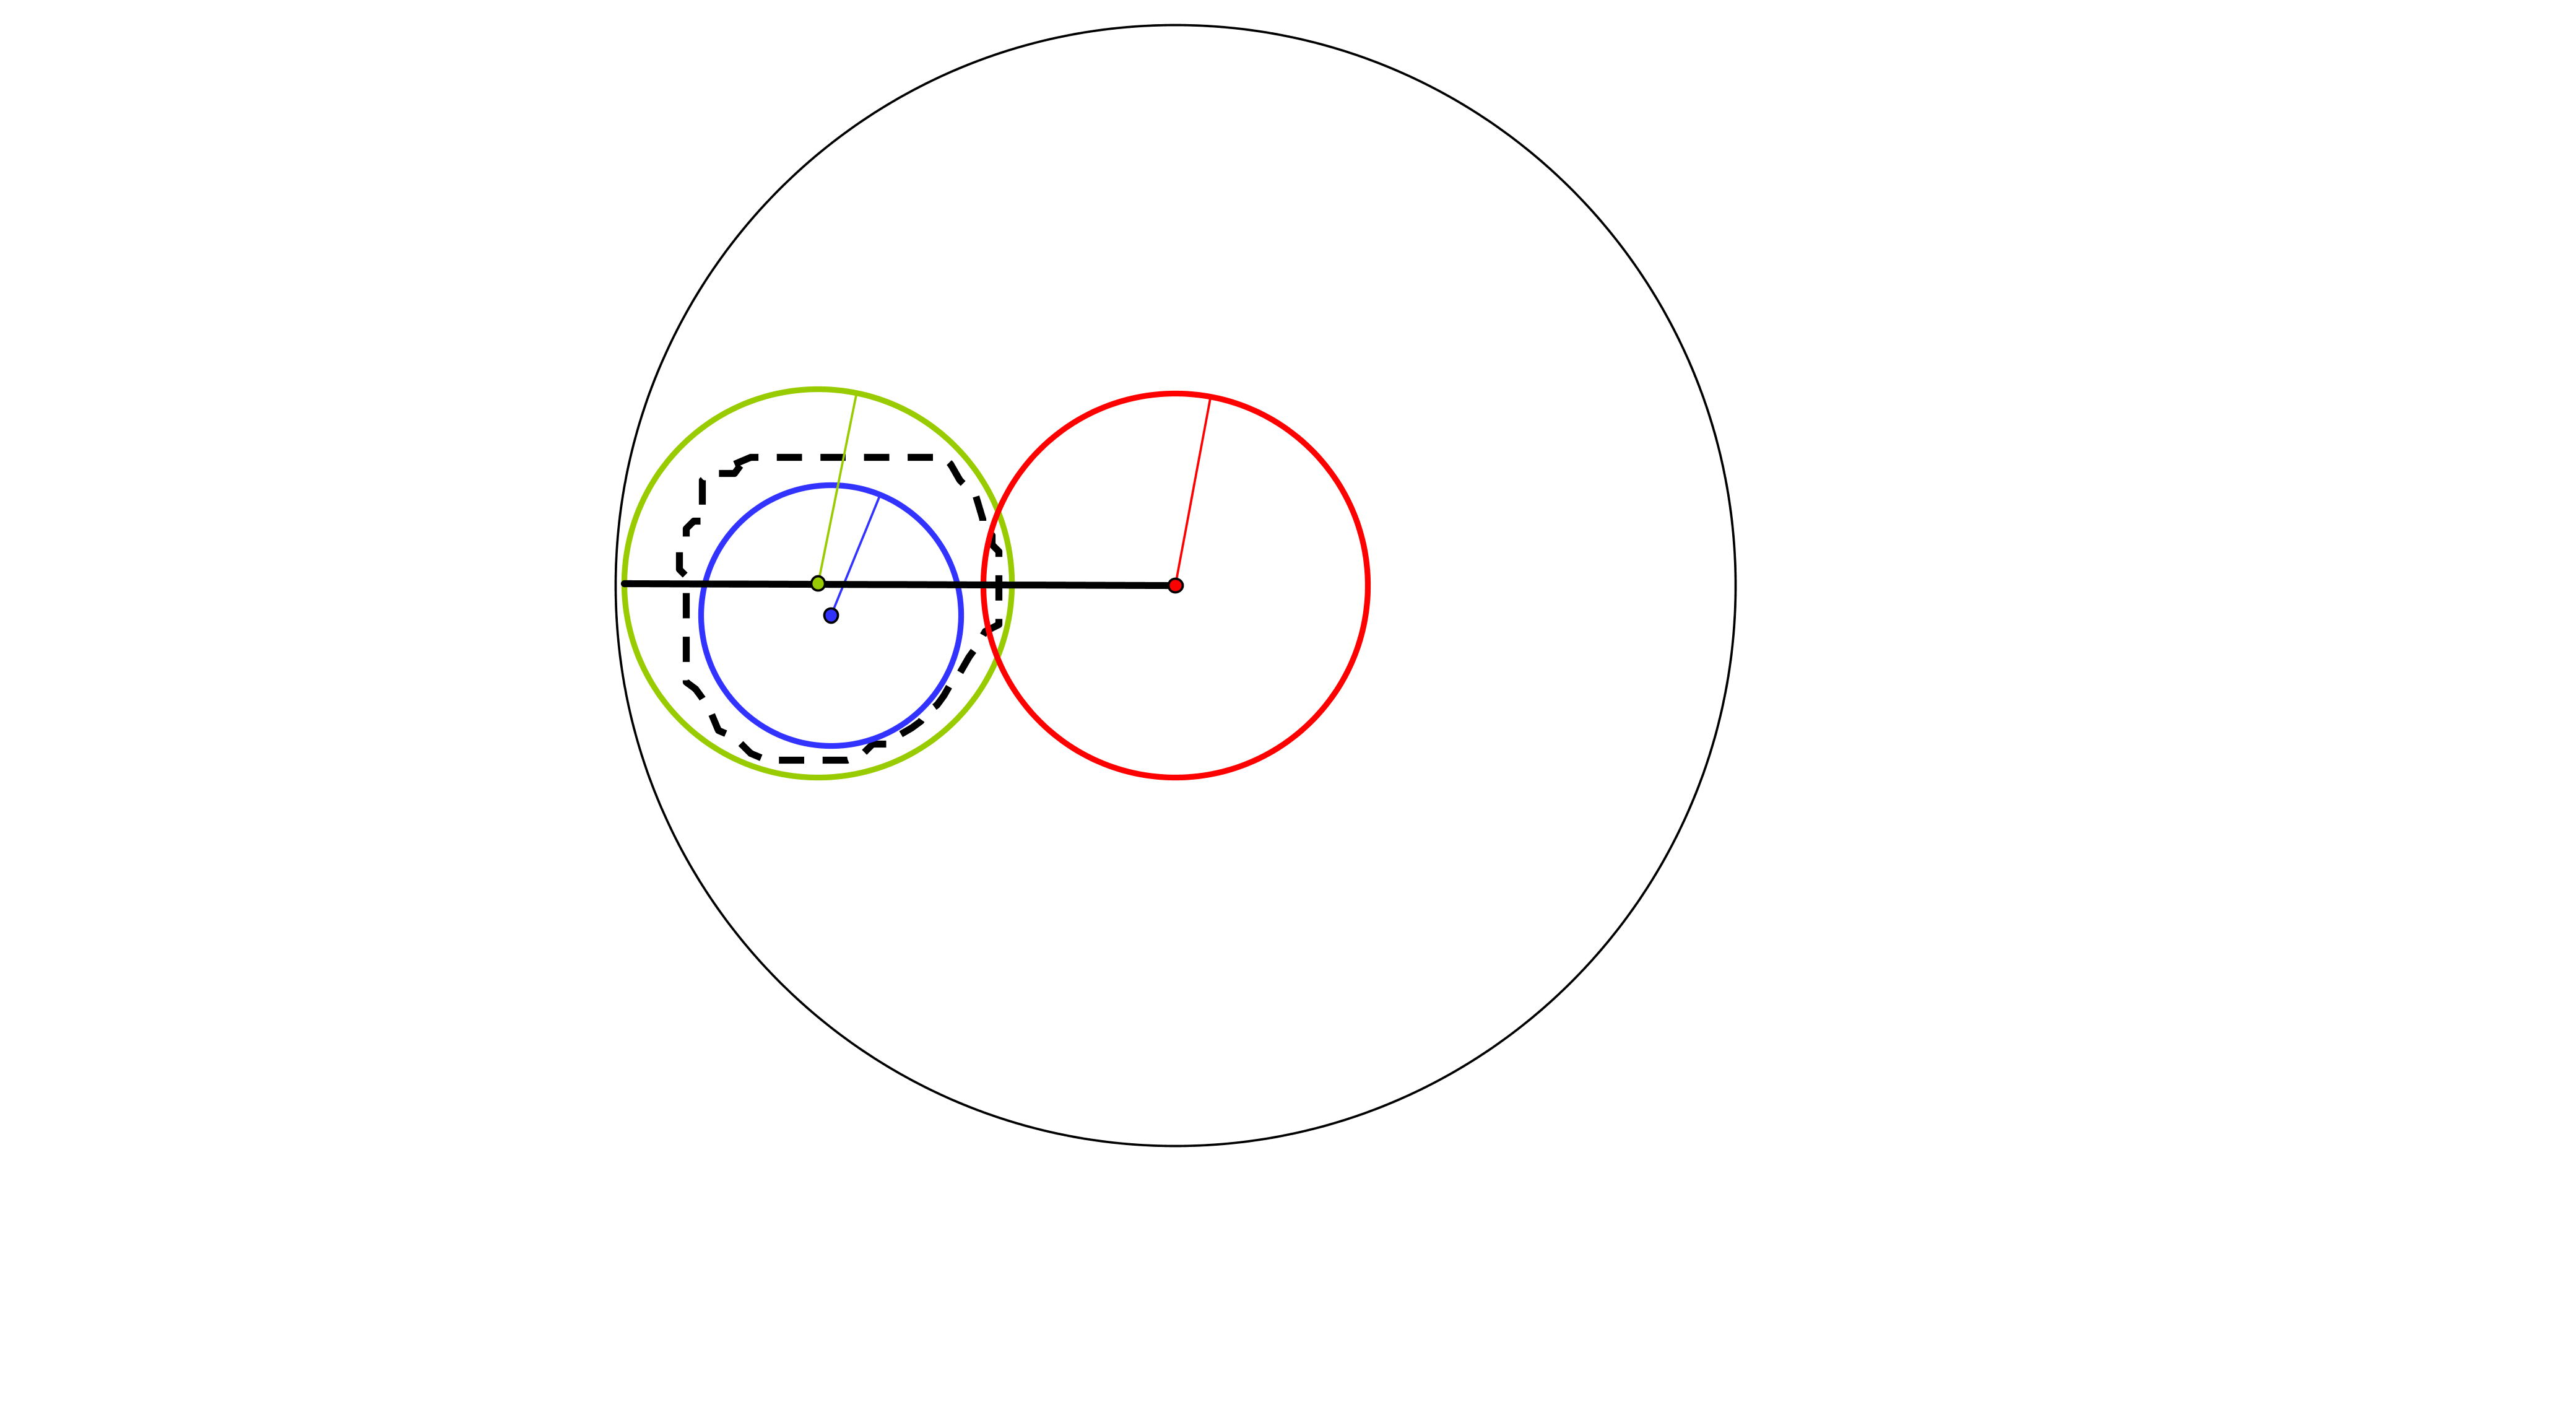
\includegraphics[width=8in]{jwk2.png}}
\put(273,178){\mbox{$B$}}
\put(270,180){\vector(-3,-1){30}}
\put(190,220){\vector(-3,-5){30}}
\put(190,220){\mbox{$V_i$}}
\put(144,155){\mbox{$a_1r$}}
\put(125,185){\mbox{$a_2r$}}
\put(220,170){\mbox{$r$}}
\end{picture}
\caption{}
\label{kola}
\end{figure}

Przypuśćmy, że $q$ zbiorów $\overline{V_i}$ przecina $B$. Sumując objętości odpowiednich wewnętrznych kul o promieniach $a_1r$, otrzymujemy wtedy:

$$q(a_1r)^n \leqslant (1+2a_2)^nr^n.$$

Czyli: $$q \leqslant (1+2a_2)^n a_1^{-n}.$$
 
\end{dow}

Kluczowym twierdzeniem, potrzebnym w dalszych rozważaniach, jest twierdzenie Banacha o punkcie stałym.

\begin{tw}{\textit{(Banacha o punkcie stałym)}}\label{banach}

Niech $(X,\rho)$ będzie przestrzenią metryczną zupełną a funkcja $f: X\longrightarrow X$ kontrakcją. Wtedy:
\begin{enumerate}
\item $f$ ma dokładnie jeden punkt stały $x_0$, tzn. istnieje dokładnie jeden punkt $x_0 \in X$ taki, że $f(x_0)=x_0$,\\
\item dla każdego $x \in X$, ciąg $(x,f(x),f(f(x))),\ldots)$ jest zbieżny do $x_0$.
\end{enumerate}

\end{tw}

\chapter{Iterowane układy funkcyjne}

\begin{df}
Iterowanym układem funkcyjnym (IFS - \textit{iterated function system}) nazywamy rodzinę kontrakcji $\lbrace S_1,\ldots,S_m\rbrace$ taką, że $S_i:\hspace{1mm} D \longrightarrow D$, gdzie $D\subset\mathbb{R}^n$.
\end{df}

\begin{tw}
Rozważmy IFS określony na zbiorze $D \subset \mathbb{R}^{n}$ kontrakcjami $ \lbrace S_1, \ldots,S_m \rbrace $. Wtedy istnieje jednoznacznie wyznaczony atraktor $F$, tj. niepusty i zwarty zbiór taki, że:

\begin{equation}\label{d1}
F = \bigcup^{m}_{i=1}{S_i(F)} 
\end{equation}

Jeśli dodatkowo zdefiniujemy przekształcenie $S$ na klasie $X$ niepustych i zwartych podzbiorów~$D$ jako:

\begin{equation}\label{d3}
\forall_{E \in X} \hspace{5mm} S(E) = \bigcup^{m}_{i=1} S_i(E)
\end{equation}

oraz oznaczymy przez $S^k$  $k$-tą iterację $S$ tzn. 

$$ 
\left\{ 
\begin{array}{l}
S^0(E) = E ,\\
S^k(E) = S\left(S^{k-1}(E)\right) \hspace{4mm}\textrm{dla} \hspace{2mm} k \geq 1, 
\end{array}
\right.
$$

wtedy:

\begin{equation}\label{d2}
\forall_{E \in X \hspace{2mm} \textrm{takiego, że} \hspace{2mm} \forall_{i=1,\ldots ,m} \hspace{2mm} S_i(E) \subset E} \hspace{5mm} F = \bigcap^{\infty}_{k=0} S^k(E).
\end{equation}
\end{tw}

Przedstawimy dwa dowody powyższego twierdzenia.

\begin{dow1}

Niech $S_1,\ldots ,S_m$ będą kontrakcjami. Oznaczmy ich stałe kontrakcji odpowiednio przez $c_1,\ldots,c_m$. Zauważmy, że $S$ przekształca zbiory z $X$ na zbiory z $X$. Do dowodu wykorzystamy poniższy fakt.

\begin{lem}\label{tp1}
Jeśli wszystkie przekształcenia $S_1,\ldots ,S_m$: $D \longrightarrow D$ są kontrakcjami, to
przekształcenie $S=\bigcup^{m}_{i=1} S_i \textrm{:} \hspace{2mm} X\longrightarrow X$ też jest kontrakcją w metryce Hausdorffa. 
\end{lem}

\begin{dow}

Przypomnijmy, że $D$ jest domkniętym podzbiorem $\mathbb{R}^n$, a $X$ jest klasą niepustych i zwartych podzbiorów $D$.

Istnieje liczba $c=\max_{1\leqslant i\leqslant m}{c_i}<1$ taka, że:
$$ 
\forall_{p,q \in D} \hspace{2mm} \forall_{i=1,\ldots ,m} \hspace{5mm} \vert S_i(p)-S_i(q)\vert \leqslant c \vert p-q \vert. 
$$

Niech $A,B \in X$ i ustalmy dowolny $\epsilon>0$. Wtedy:
$$ 
\forall_{p \in A} \hspace{2mm} \exists_{q \in B} \hspace{5mm} \vert p-q \vert \leqslant \rho(A,B)+\epsilon,
$$
gdzie $\rho$ jest metryką Hausdorffa. Oznaczmy $\rho(A,B)$ jako $\delta$. Przykładowym punktem $q$ będzie należący do $B$ środek koła o promieniu $\delta+\epsilon$, które zawiera punkt $p$. 

Wówczas:

$$
\forall_{i=1,\ldots ,m} \hspace{5mm} \vert S_i(p)-S_i(q) \vert \leqslant c \vert p-q \vert \leqslant c(\rho(A,B)+\epsilon)=c(\delta+\epsilon).
$$

Czyli: 
$$
S_i(A) \subset \left(S_i(B)\right)_{c(\delta+\epsilon)}.
$$

Stąd: 
$$ 
\hspace{2mm} S(A)=\bigcup^{m}_{i=1} S_i(A) \subset \bigcup^{m}_{i=1} \left(S_i(B)\right)_{c(\delta+\epsilon)} \subset \left(\bigcup^{m}_{i=1} S_i(B)\right)_{c(\delta+\epsilon)} = \left(S(B)\right)_{c(\delta+\epsilon)}.  
$$

Analogicznie $S(B) \subset \left(S(A)\right)_{c(\delta+\epsilon)}$.

Zatem: 
$$
\rho\left(S(A),S(B)\right)\leqslant c(\delta+\epsilon) = c(\rho(A,B)+\epsilon).
$$

A ponieważ $\epsilon>0$ był dowolny, więc $\rho\left(S(A),S(B)\right)\leqslant c\rho(A,B)$. $S$ jest więc rzeczywiście kontrakcją.

\end{dow}

Wróćmy teraz do dowodu naszego twierdzenia.
Wiemy już, że $S$ jest kontrakcją na $(X,\rho)$, natomiast $\rho$ jest zupełną metryką na $X$ (patrz Twierdzenie~\ref{zup}). Spełnione są więc założenia Twierdzenia~\ref{banach} -- twierdzenia Banacha o punkcie stałym.
Zatem, jako wniosek z tego twierdzenia, otrzymujemy, że $S$ ma jednoznacznie wyznaczony punkt stały $F$. Czyli $S(F)=F$, co dowodzi równości~\eqref{d1}.

Co więcej, $S^k(E)\longrightarrow F$, gdy $k\longrightarrow\infty$, dla dowolnego zbioru $E \in X$. W szczególności, jeśli $S_i(E) \subset E$ dla każdego $i$, wtedy $S(E) \subset E$ i $\lbrace S^k(E)\rbrace^{\infty}_{k=1}$ jest zstępującą rodziną zbiorów niepustych i zwartych. Czyli $F = \bigcap^{\infty}_{k=0} S^k(E)$, co dowodzi równości \eqref{d2}.

\end{dow1}

\begin{dow2}

Niech $E \in X$ będzie zbiorem takim, że $S_i(E) \subset E$ dla każdego $i=1,\ldots ,m$. Taki zbiór istnieje -- weźmy na przykład $E=D \cap \overline{B}(0,r)$ dla odpowiednio dużego $r>0$. Uzasadnimy, że da się tak dobrać $r$, aby zbiór $E$ spełniał żądany warunek.

Wiemy, że $S_i(D) \subset D$ (z definicji $S_i$). Jeśli znajdziemy takie $r>0$, dla którego $S_i(\overline{B}(0,r)) \subset \overline{B}(0,r)$, wtedy będziemy mieć, że $S_i(D \cap \overline{B}(0,r)) \subset D \cap \overline{B}(0,r)$.

Jeśli przyjmiemy, że $y_i:=S_i(0)$, wtedy:
$$
S_i(\overline{B}(0,r))\subset\overline{B}(y_i,c_ir).
$$

Wynika to z poniższej nierówności:
$$ 
|y_i-S_i(x)|=|S_i(0)-S_i(x)|\leqslant c_i|0-x|=c_i|x|\leqslant c_ir, 
$$
gdzie $x \in \overline{B}(0,r)$.

Chcemy, żeby $S_i(\overline{B}(0,r))\subset\overline{B}(y_i,c_ir)\subset\overline{B}(0,r)$. Szacujemy więc $r$ w następujący sposób:

$$
\aligned
r&> \vert y_i \vert + c_ir\\
r(1-c_i)&>\vert y_i \vert\\
r&>\frac{\vert y_i \vert}{1-c_i}\textrm{, bo }c_i<1
\endaligned
$$

Zatem dla odpowiednio dużego $r$ wybrany zbiór $E=D \cap \overline{B}(0,r)$ spełnia warunek $S_i(E)~\subset~E$.

Wtedy $S^k(E) \subset S^{k-1}(E)$ dla dowolnego $k \geqslant 1$.

Czyli $\lbrace S^k(E) \rbrace^{\infty}_{k=0}$ jest zstępującą rodziną zbiorów niepustych i zwartych (bo $E$ jest domknięty -- jako przecięcie zbiorów domkniętych -- i ograniczony), więc przecięcie $F = \bigcap^{\infty}_{k=0} S^k(E)$ jest niepuste i zwarte. Wynika to z twierdzenia, że zstępująca rodzina zbiorów domkniętych ma niepuste przecięcie.

Wtedy:
$$
S(F)=S\left(\bigcap^{\infty}_{k=0} S^k(E)\right)=\bigcap^{\infty}_{k=0} S(S^k(E))=\bigcap^{\infty}_{k=0} S^{k+1}(E)=\bigcap^{\infty}_{n=1} S^n(E)=\bigcap^{\infty}_{n=0} S^n(E)=F.
$$

Tak więc $F$ spełnia równość \eqref{d3}, czyli jest atraktorem IFS. Sprawdźmy, czy jest atraktorem  wyznaczonym jednoznacznie.

Niech $A,B$ będą atraktorami IFS, w szczególności: $S(A)=A$ oraz $S(B)=B$.

Ponieważ $S$ jest kontrakcją ze stałą $c=\max_{1\leqslant i\leqslant m}{c_i}$, $0<c<1$ (patrz Lemat~ \ref{tp1}), więc:
$$
\aligned
\rho(S(A),S(B))&\leqslant c\rho(A,B)\\
\rho(A,B) &\leqslant c\rho(A,B)\\
\rho(A,B)-c\rho(A,B)&\leqslant 0\\
\rho(A,B)(1-c)&\leqslant 0
\endaligned
$$

Ponieważ $c<1$, to $\rho(A,B)\leqslant 0$.
Zatem $\rho(A,B)=0$. Z definicji metryki wiemy zaś, że wtedy $A=B$.
\end{dow2}


\chapter{Twierdzenie o wymiarze fraktali}

\begin{df}\label{osc}
Funkcje $S_1,\ldots,S_m$ takie, że $S_i:D \longrightarrow D$, spełniają warunek zbioru otwartego (\textit{open set condition}), jeśli istnieje niepusty, ograniczony i otwarty zbiór $V$ taki, że:
$$
\bigcup^{m}_{i=1}S_i(V) \subset V
$$

oraz $S_i(V)$ są parami rozłączne dla $i=1,\ldots,m$. 
\end{df}

\begin{tw}\label{wym}
Przypuśćmy, że podobieństwa $S_1,\ldots,S_m$ określone na $\mathbb{R}^n$ ze stałymi $c_i \in (0,1)$ dla $i=1,\ldots,m$, spełniają warunek zbioru otwartego.

Jeśli $F$ jest atraktorem IFS $\lbrace S_1,\ldots,S_m\rbrace$ tzn. 
$$
F = \bigcup^{m}_{i=1}{S_i(F)},
$$

wtedy $\dim_HF=s$, gdzie $s$ jest rozwiązaniem równania:

\begin{equation}\label{s}
\sum^m_{i=1}c_i^s=1.
\end{equation}

Co więcej, dla tej wartości $s$, $0<\mathcal{H}^s(F)<\infty$.
\end{tw}


\begin{dow}

Niech $s$ spełnia \eqref{s} tzn. $\sum^m_{i=1}c_i^s=1$. 

Niech $I_k$ będzie zbiorem zawierającym ciągi długości $k$ o elementach ze zbioru $\lbrace 1,\ldots,m\rbrace$.

Dla dowolnego zbioru $A$ i dla każdego ciągu $(i_1,\ldots,i_k)\in I_k$ definiujemy:
$$
A_{i_1,\ldots,i_k}=S_{i_1}\circ\ldots\circ S_{i_k}(A)=S_{i_1}(\ldots(S{i_k}(A))\ldots).
$$

Zauważmy, że wtedy:  
$$
F=\bigcup_{I_k}F_{i_1,\ldots,i_k}.
$$ 

Poniżej przedstawię krótkie uzasadnienie tego faktu.
$$
F\stackrel{\eqref{d2}}{=}\bigcap^{\infty}_{k=0}S^k(F)=\bigcap^{\infty}_{k=0}\bigcup_{I_k} S_{i_1}\circ\ldots\circ S_{i_k}(F)=\bigcap^{\infty}_{k=0}\bigcup_{I_k}F_{i_1,\ldots,i_k},
$$
czyli $F\subset\bigcup_{I_k}F_{i_1,\ldots,i_k}$. A ponieważ $F_{i_1,\ldots,i_k}\subset F$, więc $\bigcup_{I_k}F_{i_1,\ldots,i_k}\subset F$, czyli ostatecznie $F=\bigcup_{I_k}F_{i_1,\ldots,i_k}$ dla każdego $k$.

Otrzymujemy więc pewne pokrycie $F$. Dzięki niemu dostaniemy górne ograniczenie miary i wymiaru Hausdorffa atraktora. 

Zauważmy najpierw, że $S_{i_1}\circ\ldots\circ S_{i_k}$ jest podobieństwem o stałej $c_{i_1}\cdot\ldots\cdot c_{i_k}$.

Wtedy mamy, że:
$$
\aligned
\sum_{I_k}|F_{i_1,\ldots,i_k}|^s&=\sum_{I_k}|S_{i_1}\circ\ldots\circ S_{i_k}(F)|^s=\sum_{I_k}(c_{i_1}\cdot\ldots\cdot c_{i_k}|F|)^s= \sum_{I_k}(c_{i_1}\cdot\ldots\cdot c_{i_k})^s{|F|}^s = \\
&=\left(\sum_{i_1}c_{i_1}^s\right)\cdot \ldots\cdot\left(\sum_{i_k}c_{i_k}^s\right)|F|^s=1\cdot\ldots\cdot1\cdot|F|^s=|F|^s.
\endaligned
$$

Tak więc pokazaliśmy, że:
$$
\sum_{I_k}|F_{i_1,\ldots,i_k}|^s=|F|^s,
$$
gdzie $\lbrace F_{i_1,\ldots,i_k}\rbrace$ jest pokryciem $F$. Dla każdej $\delta>0$ możemy wybrać $k$ takie, że: 
$$
|F_{i_1,\ldots,i_k}|\leqslant c^k|F|\leqslant\delta,
$$
gdzie $c=\max_{1\leqslant i\leqslant m}{c_i}$.

Wynika to z poniższego rachunku:
$$
|F_{i_1,\ldots,i_k}|=|S_{i_1}\circ\ldots\circ S_{i_k}(F)|=c_{i_1}\ldots c_{i_k}|F| \leqslant \left(\max_{1\leqslant i\leqslant m}{c_i}\right)^k|F|\leqslant c^k|F|\leqslant\delta
$$ 
dla odpowiednio dużego $k$, gdyż $c \in (0,1)$.

Ponieważ $\mathcal{H}^s_{\delta}(F)=\inf\sum_i|U_i|^s$, gdzie infimum jest jest wzięte po wszystkich $\delta$-pokryciach $F$, a $\lbrace F_{i_1,\ldots,i_k}\rbrace$ jest $\delta$-pokryciem $F$, więc:
$$
\mathcal{H}^s_{\delta}(F)\leqslant \sum_{I_k}|F_{i_1,\ldots,i_k}|^s=|F|^s.
$$

Zatem $\displaystyle\mathcal{H}^s(F)=\lim_{\delta\rightarrow 0^+}\mathcal{H}^s_{\delta}(F)\leqslant|F|^s<\infty$ oraz $\displaystyle\dim_H(F)=\inf\lbrace t: \mathcal{H}^t(F)=0\rbrace \leqslant s$. 

Uzyskanie dolnego ograniczenia będzie trochę bardziej skomplikowane.

Zdefiniujemy zbiór $I = \lbrace (i_1 , i_2 , \ldots ): 1 \leqslant i_j \leqslant m \rbrace $, czyli zbiór ciągów nieskończonych o wyrazach z $ \lbrace 1 , \ldots , m \rbrace $ oraz zbiór $J_{i_1 , \ldots , i_k}=\lbrace(i_1 ,\ldots,i_k,q_{k+1},q_{k+2} \ldots):~1\leqslant~i_j\leqslant~m,~1\leqslant~q_j\leqslant~m\rbrace$, czyli zbiór ciągów nieskończonych o ustalonych~$k$ pierwszych wyrazach (tzw. cylinder długości~$k$).

Możemy teraz zdefiniować miarę $\mu$ na pewnych podzbiorach $I$. Żeby to zrobić definiujemy najpierw funkcję $\mu$ na cylindrach $J_{i_1, \ldots , i_k}$, a następnie rozszerzymy ją na $\sigma$-ciało generowane przez cylindry. Niech więc:
$$
\mu ( J_{i_1, \ldots , i_k} ) := (c_{i_1} \cdot \ldots \cdot c_{i_k})^s .
$$

Zauważmy, że: 
$$ 
(c_{i_1} \cdot \ldots \cdot c_{i_k})^s = \sum^m_{i=1} (c_{i_1} \cdot \ldots \cdot c_{i_k} \cdot c_i)^s.
$$ 

Wynika to z poniższych równości:
$$ 
\sum^m_{i=1} (c_{i_1} \cdot \ldots \cdot c_{i_k} \cdot c_i)^s = (c_{i_1} \cdot \ldots \cdot c_{i_k})^s \sum^m_{i=1} c_i^s = (c_{i_1} \cdot \ldots \cdot c_{i_k})^s \cdot 1 = (c_{i_1} \cdot \ldots \cdot c_{i_k})^s 
$$

A zatem:
$$ 
\mu ( J_{i_1, \ldots , i_k} ) = (c_{i_1} \cdot \ldots \cdot c_{i_k})^s = \sum^m_{i=1} (c_{i_1} \cdot \ldots \cdot c_{i_k} \cdot c_i)^s = \sum^m_{i=1} \mu (J_{i_1, \ldots , i_k,i}).
$$

Czyli:
$$ 
\mu ( J_{i_1, \ldots , i_k} ) = \sum^m_{i=1} \mu (J_{i_1, \ldots , i_k,i}).
$$

Wynika z tego, że $\mu$ jest funkcją $\sigma$-addytywną na ciele zbiorów zawierających cylindry. Można również zauważyć, że:
$$ 
\aligned 
\mu (I) &= \sum_{I_k} \mu ( J_{i_1, \ldots , i_k} ) = \sum_{I_k} \sum^m_{i=1} \mu (J_{i_1, \ldots , i_k,i}) = \sum_{I_k} \sum^m_{i=1} (c_{i_1} \cdot \ldots \cdot c_{i_k} \cdot c_i)^s =\\
&= \left( \sum_{i_1} c_{i_1}^s \right) \cdot \ldots \cdot \left( \sum_{i_k} c_{i_k}^s \right) \cdot \left( \sum^{m}_{i=1} c_{i}^s \right) = 1 \cdot \ldots \cdot 1 = 1.
\endaligned 
$$

Zatem $\mu ( I ) = 1$. 

Następnym krokiem jest zdefiniowanie miary zewnętrznej $\mu^*$ na $2^I$: 
$$
\mu^*(C)=\inf \left\lbrace \sum_{i=1}^{\infty} \mu(A_i): A_i\textrm{ -- cylindry oraz } C \subset \bigcup_{i=1}^{\infty} A_i \right\rbrace.
$$

Na mocy twierdzenia Carath\'eodory'ego obcięcie $\mu^*$ do $\sigma$-ciała zbiorów mierzalnych (generowanego przez cylindry) jest miarą. Będziemy ją oznaczali $\mu$. 
 

Niech $E$ będzie zwartym podzbiorem $\mathbb{R}^n$. Jeśli $S_i(E)\subset E$ dla każdego $i=1,\ldots,m$, a $x \in F$, to z \eqref{d2} wynika, że istnieje ciąg $(i_1,i_2,\ldots)$, niekoniecznie jedyny, taki, że $x \in S_{i_1}\circ\ldots\circ S_{i_k} (E)$ dla każdego $k$. Ten ciąg pozwala zdefiniować pewne naturalne kodowanie dla $x$. Mianowicie $\lbrace x\rbrace=\lbrace x_{i_1,i_2, \ldots}\rbrace=\bigcap^{\infty}_{k=1} S_{i_1}\circ\ldots\circ S_{i_k} (E)$. Wtedy $F=\bigcup_I \lbrace x_{i_1,i_2, \ldots} \rbrace$. Dzięki temu kodowaniu, możemy w naturalny sposób przekształcić miarę $\mu$ zdefiniowaną na $\sigma$-ciele generowanym przez cylindry na miarę $ \tilde{\mu} $ zdefiniowaną na podzbiorach $F$ w sposób opisany poniżej.

Zdefiniujmy rzutowanie $\Pi: I \longrightarrow F$ w następujący sposób:
$$
\Pi(i_1,i_2,\ldots)=\bigcap^{\infty}_{k=1} F_{i_1, \ldots, i_k}.
$$
Zauważmy, że $\Pi$ jest "na", ale niekoniecznie "1-1". 

Dla zbiorów $A$ takich, że przeciwobraz $\Pi^{-1}(A)$ jest $\mu$-mierzalny, możemy zdefiniować:
$$
\tilde{\mu}(A) = \mu (\Pi^{-1}(A)). 
$$

Tak więc miara $\tilde{\mu}$ zbioru jest miarą $\mu$ kodów elementów należących do tego zbioru.
Widać zatem, że $\tilde{\mu}(F)=1$.

Wprowadźmy topologię na $I$ jako najmniejszą topologię zawierającą wszystkie cylindry. Można pokazać, że wtedy $\Pi$ jest ciągłe. A z tego wynika, że $\tilde{\mu}$ jest miarą borelowską.

Pokażemy teraz, że $\tilde{\mu}$ spełnia założenia Twierdzenia~\ref{mass}.

Niech $V$ będzie zbiorem z definicji warunku zbioru otwartego, czyli $S(V) \subset V$, $V$ -- niepusty, ograniczony i otwarty oraz $S_i(V)$ są parami rozłączne.

Z ciągłości podobieństw $S_i$ wiemy, że:
$$
\bigcup^m_{i=1} S_i\left(\overline{V}\right) = S\left(\overline{V}\right) \subset \overline{V}.
$$ 

Na mocy \eqref{d2}, $ F = \bigcap^{\infty}_{k=0} S^k(\overline{V}) $, bo $S(\overline{V})\subset \overline{V}$ oraz $\overline{V}$ jest niepusty, domknięty i ograniczony, czyli niepusty i zwarty w $\mathbb{R}^n$.

W szczególności $ F \subset \overline{V} $ oraz 

\begin{equation}\label{zaw}
F_{i_1,\ldots,i_k}\subset \overline{V}_{i_1,\ldots,i_k},
\end{equation}

gdyż $ F_{i_1,\ldots,i_k}=S_{i_1}\circ\ldots\circ S_{i_k}(F) \subset S_{i_1}\circ\ldots\circ S_{i_k}(\overline{V})=\overline{V}_{i_1,\ldots,i_k} $ dla każdego ciągu $(i_1\ldots,i_k)$.

Niech $B$ będzie kulą o ustalonym promieniu $0<r<1$.

Szacujemy $\tilde{\mu}(B)$ rozważając zbiory $ V_{i_1,\ldots,i_k} $ o średnicach porównywalnych z $|B|$ i z domknięciami przecinającymi $F \cap B$.

Obcinamy każdy nieskończony ciąg $(i_1,i_2,\ldots) \in I$ po pierwszym wyrazie $i_k$, dla którego:

\begin{equation}\label{rrr}
\left(\min_{1 \leqslant i \leqslant m} c_i\right)\cdot r \leqslant c_{i_1} c_{i_2 }\ldots c_{i_k} \leqslant r
\end{equation}

Takie $i_k$ będzie istniało dla każdego ciągu. Wynika to z poniższej konstrukcji. 
 
Weźmy dowolny ciąg $(i_1,i_2,\ldots) \in I$. Niech $k$ będzie najmniejszym indeksem, dla którego $c_{i_1}\ldots c_{i_k} \leqslant r$. 

Dla $k>1$ mamy wtedy $c_{i_1}\ldots c_{i_{k-1}} > r$, zatem:
$$
\displaystyle c_{i_1}\ldots c_{i_{k-1}}\cdot c_{i_k} > r \cdot c_{i_k} \geqslant r \cdot \left(\min_{1\leqslant i\leqslant m} c_i\right)
$$

Niech $Q$ stanowi zbiór wszystkich skończonych ciągów otrzymanych w ten sposób. Q jest skończony, bo dla $0<r<1$:
$$
\exists_{K>0} \hspace{3mm} \left(\max_{{1\leqslant i\leqslant m}} c_i\right)^K \leqslant r. 
$$

Czyli długość ciągów z $Q$ nie przekracza $K$. Skończonych ciągów długości nie większej niż $K$ o wyrazach z $\lbrace 1,\ldots,m\rbrace$ jest nie więcej niż $m^k$, czyli skończenie wiele.

Zatem, przy tak zdefiniowanym $Q$, dla każdego nieskończonego ciągu  $(i_1,i_2,\ldots)\in I$ istnieje dokładnie jedna wartość $k$, dla której $(i_1,\ldots,i_k) \in Q$.

Ponieważ zbiory $V_1,\ldots,V_m$, gdzie $V_j=S_j(V)$, są parami rozłączne (patrz Definicja~\ref{osc}), więc $V_{i_1,\ldots,i_k,1},\ldots,V_{i_1,\ldots,i_k,m}$ też są parami rozłączne dla każdego $(i_1,\ldots,i_k) \in Q$.

A zatem zbiory otwarte $ V_{i_1,\ldots,i_k} $ dla $(i_1,\ldots,i_k) \in Q$ są parami rozłączne.

Zatem: 
$$ 
F \subset \bigcup_Q F_{i_1,\ldots,i_k} \subset \bigcup_Q \overline{V}_{i_1,\ldots,i_k}.
$$

Drugie zawieranie otrzymujemy natychmiast z \eqref{zaw}. Pierwsze natomiast krótko wyjaśnimy poniżej.

Niech $x \in F$. Wtedy punktowi $x$ można przypisać kod $ (i_1,i_2,i_3,\ldots) $ taki, że $x \in F_{i_1,\ldots,i_k}$ dla każdego $k$. Gdy go obetniemy po pierwszym $i_k$ spełniającym \eqref{rrr}, to otrzymamy, że $x \in F_{i_1,\ldots,i_k}$, gdzie $(i_1,\ldots,i_k)\in Q$.

Wybieramy teraz $a_1>0$ i $a_2>0$ takie, że $V$ zawiera kulę o promieniu $a_1$ (to jest możliwe, bo $V$ jest otwarty) oraz jest zawarty w kuli o promieniu $a_2$ (to jest możliwe, bo $V$ jest ograniczony).

Wtedy dla każdego $ (i_1,\ldots,i_k)\in Q $, zbiór $V_{i_1,\ldots,i_k}$ zawiera kulę o promieniu $c_{i_1}\cdot\ldots\cdot c_{i_k}\cdot a_1$, a zatem również kulę o promieniu $a_1\cdot r\cdot \min_{1\leqslant i \leqslant m} c_i$ -- na mocy \eqref{rrr} -- oraz jest zawarty w kuli o promieniu $c_{i_1}\cdot\ldots\cdot c_{i_k}\cdot a_2$, a zatem również w kuli o promieniu $a_2 r$.

Niech $Q_1$ będzie zbiorem tych ciągów $(i_1,\ldots,i_k)\in Q$, dla których $B$ przecina $ \overline{V}_{i_1,\ldots,i_k} $. Korzystając z Twierdzenia~\ref{apple}, mamy co najwyżej $q = (1+2a_2)^na_1^{-n}(\min_i c_i)^{-n}$ ciągów w $Q_1$. Wtedy:
$$ 
\tilde{\mu}(B) := \tilde{\mu}(F \cap B) = \mu(\lbrace (i_1,i_2,\ldots): x_{i_1,i_2,\ldots} \in F \cap B \rbrace) \leqslant \mu \left(\bigcup_{Q_1} I_{i_1,\ldots,i_k}\right).  
$$

Na Rysunku~\ref{fb} łatwo widać, dlaczego $F\cap B \subset \bigcup_{Q_1} F_{i_1,\ldots,i_k}$.

\begin{figure}[h]
\begin{picture}(500,250)
\put(50,50){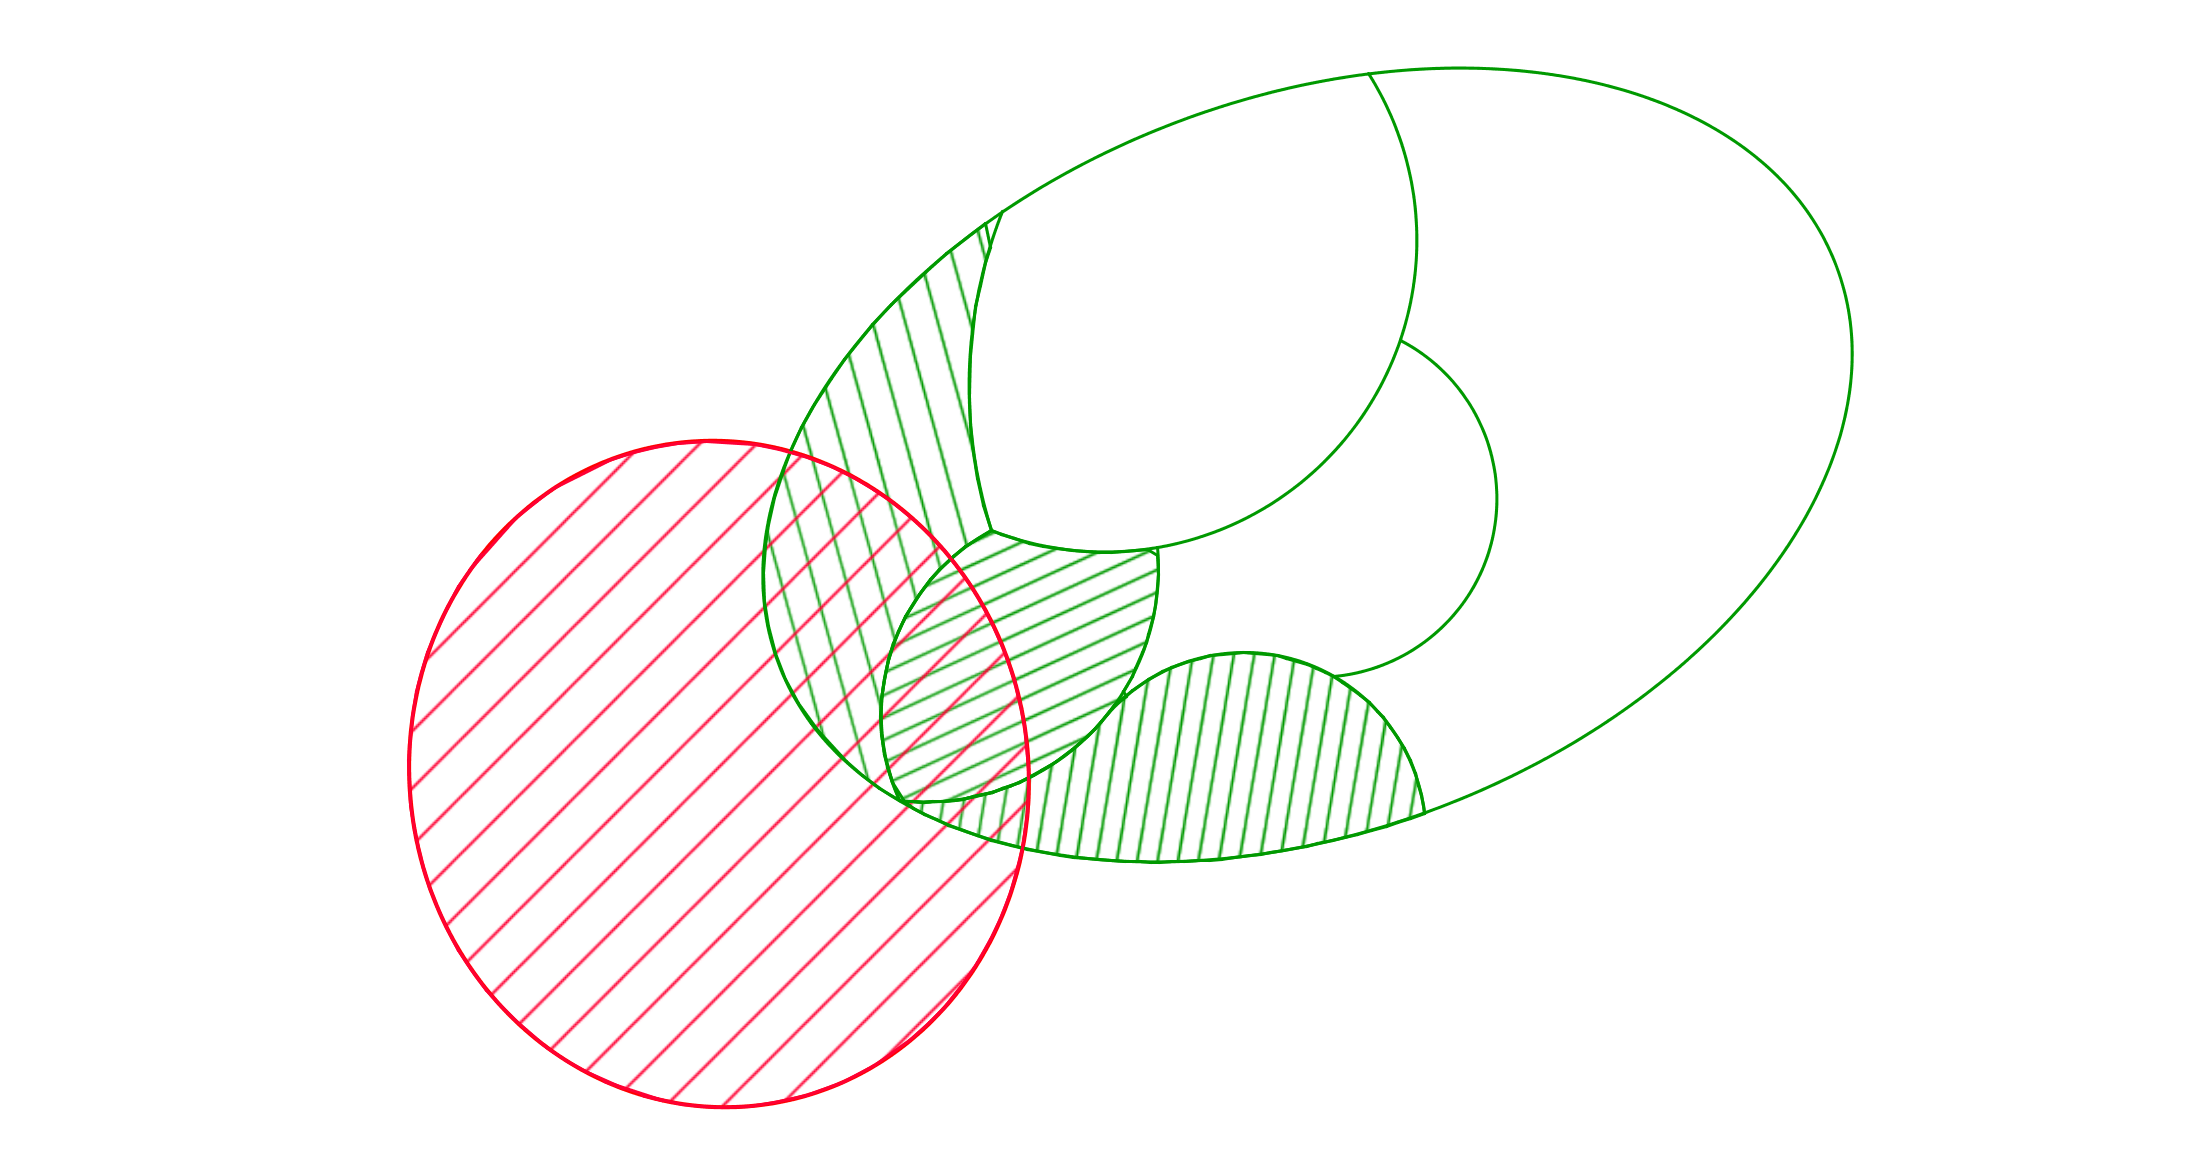
\includegraphics[width=4in]{obr.png}}
\put(120,200){\mbox{$\bigcup_{Q_1} F_{i_1,\ldots,i_k}$}}
\put(140,190){\vector(3,-5){30}}
\put(325,150){\mbox{$F$}}
\put(320,152){\vector(-1,0){80}}
\put(70,150){\mbox{$B$}}
\put(81,152){\vector(5,-4){50}}
\put(200,50){\mbox{$F\cap B$}}
\put(215,60){\vector(-5,6){40}}
\end{picture}
\caption{}
\label{fb}
\end{figure}

Tak więc: 
$$
\tilde{\mu}(B)\leqslant\sum_{Q_1}\mu(I_{i_1,\ldots,i_k}) = \sum_{Q_1} (c_{i_1}\ldots c_{i_k})^s \leqslant \sum_{Q_1} r^s \leqslant qr^s.
$$

Ponieważ dowolny zbiór $U$ jest zawarty w kuli o promieniu $|U|$, zatem:
$$
\tilde{\mu}(U)\leqslant|U|^sq.
$$

Tak więc z Twierdzenia~\ref{mass} mamy: $\mathcal{H}^s(F)\geqslant \frac{1}{q}>0$ oraz $\dim_HF\geqslant s$.

Czyli ostatecznie $\dim_HF = s$ oraz $0<\mathcal{H}^s(F)<\infty$.
\end{dow}


\chapter{Przykłady}

W tym rozdziale przytoczę trzy przykłady zastosowania Twierdzenia~\ref{wym}. 

\section{Przykład 1.}

Pierwszy przykład obrazuje sytuację, gdy wszystkie stałe podobieństwa są takie same. Przeanalizujmy fraktal zwany trójkątem Sierpińskiego -- Rysunek~\ref{p1}. 

\begin{figure}[h]
\begin{center}
\begin{picture}(250.00,250.00)
{\color{black}\polygon*(0.00,150.00)(50.00,236.60)(100.00,150.00) \polygon*(150.00,150.00)(175.00,193.30)(200.00,150.00) \polygon*(175.00,193.30)(200.00,236.60)(225.00,193.30) \polygon*(200.00,150.00)(225.00,193.30)(250.00,150.00) \polygon*(0.00,25.00)(12.50,46.65)(25.00,25.00) \polygon*(12.50,46.65)(25.00,68.30)(37.50,46.65) \polygon*(25.00,25.00)(37.50,46.65)(50.00,25.00) \polygon*(25.00,68.30)(37.50,89.95)(50.00,68.30) \polygon*(37.50,89.95)(50.00,111.60)(62.50,89.95) \polygon*(50.00,68.30)(62.50,89.95)(75.00,68.30) \polygon*(50.00,25.00)(62.50,46.65)(75.00,25.00) \polygon*(62.50,46.65)(75.00,68.30)(87.50,46.65) \polygon*(75.00,25.00)(87.50,46.65)(100.00,25.00) \polygon*(150.00,25.00)(151.56,27.71)(153.12,25.00) \polygon*(151.56,27.71)(153.12,30.41)(154.69,27.71) \polygon*(153.12,25.00)(154.69,27.71)(156.25,25.00) \polygon*(153.12,30.41)(154.69,33.12)(156.25,30.41) \polygon*(154.69,33.12)(156.25,35.83)(157.81,33.12) \polygon*(156.25,30.41)(157.81,33.12)(159.38,30.41) \polygon*(156.25,25.00)(157.81,27.71)(159.38,25.00) \polygon*(157.81,27.71)(159.38,30.41)(160.94,27.71) \polygon*(159.38,25.00)(160.94,27.71)(162.50,25.00) \polygon*(156.25,35.83)(157.81,38.53)(159.38,35.83) \polygon*(157.81,38.53)(159.38,41.24)(160.94,38.53) \polygon*(159.38,35.83)(160.94,38.53)(162.50,35.83) \polygon*(159.38,41.24)(160.94,43.94)(162.50,41.24) \polygon*(160.94,43.94)(162.50,46.65)(164.06,43.94) \polygon*(162.50,41.24)(164.06,43.94)(165.62,41.24) \polygon*(162.50,35.83)(164.06,38.53)(165.62,35.83) \polygon*(164.06,38.53)(165.62,41.24)(167.19,38.53) \polygon*(165.62,35.83)(167.19,38.53)(168.75,35.83) \polygon*(162.50,25.00)(164.06,27.71)(165.62,25.00) \polygon*(164.06,27.71)(165.62,30.41)(167.19,27.71) \polygon*(165.62,25.00)(167.19,27.71)(168.75,25.00) \polygon*(165.62,30.41)(167.19,33.12)(168.75,30.41) \polygon*(167.19,33.12)(168.75,35.83)(170.31,33.12) \polygon*(168.75,30.41)(170.31,33.12)(171.88,30.41) \polygon*(168.75,25.00)(170.31,27.71)(171.88,25.00) \polygon*(170.31,27.71)(171.88,30.41)(173.44,27.71) \polygon*(171.88,25.00)(173.44,27.71)(175.00,25.00) \polygon*(162.50,46.65)(164.06,49.36)(165.62,46.65) \polygon*(164.06,49.36)(165.62,52.06)(167.19,49.36) \polygon*(165.62,46.65)(167.19,49.36)(168.75,46.65) \polygon*(165.62,52.06)(167.19,54.77)(168.75,52.06) \polygon*(167.19,54.77)(168.75,57.48)(170.31,54.77) \polygon*(168.75,52.06)(170.31,54.77)(171.88,52.06) \polygon*(168.75,46.65)(170.31,49.36)(171.88,46.65) \polygon*(170.31,49.36)(171.88,52.06)(173.44,49.36) \polygon*(171.88,46.65)(173.44,49.36)(175.00,46.65) \polygon*(168.75,57.48)(170.31,60.18)(171.88,57.48) \polygon*(170.31,60.18)(171.88,62.89)(173.44,60.18) \polygon*(171.88,57.48)(173.44,60.18)(175.00,57.48) \polygon*(171.88,62.89)(173.44,65.59)(175.00,62.89) \polygon*(173.44,65.59)(175.00,68.30)(176.56,65.59) \polygon*(175.00,62.89)(176.56,65.59)(178.12,62.89) \polygon*(175.00,57.48)(176.56,60.18)(178.12,57.48) \polygon*(176.56,60.18)(178.12,62.89)(179.69,60.18) \polygon*(178.12,57.48)(179.69,60.18)(181.25,57.48) \polygon*(175.00,46.65)(176.56,49.36)(178.12,46.65) \polygon*(176.56,49.36)(178.12,52.06)(179.69,49.36) \polygon*(178.12,46.65)(179.69,49.36)(181.25,46.65) \polygon*(178.12,52.06)(179.69,54.77)(181.25,52.06) \polygon*(179.69,54.77)(181.25,57.48)(182.81,54.77) \polygon*(181.25,52.06)(182.81,54.77)(184.38,52.06) \polygon*(181.25,46.65)(182.81,49.36)(184.38,46.65) \polygon*(182.81,49.36)(184.38,52.06)(185.94,49.36) \polygon*(184.38,46.65)(185.94,49.36)(187.50,46.65) \polygon*(175.00,25.00)(176.56,27.71)(178.12,25.00) \polygon*(176.56,27.71)(178.12,30.41)(179.69,27.71) \polygon*(178.12,25.00)(179.69,27.71)(181.25,25.00) \polygon*(178.12,30.41)(179.69,33.12)(181.25,30.41) \polygon*(179.69,33.12)(181.25,35.83)(182.81,33.12) \polygon*(181.25,30.41)(182.81,33.12)(184.38,30.41) \polygon*(181.25,25.00)(182.81,27.71)(184.38,25.00) \polygon*(182.81,27.71)(184.38,30.41)(185.94,27.71) \polygon*(184.38,25.00)(185.94,27.71)(187.50,25.00) \polygon*(181.25,35.83)(182.81,38.53)(184.38,35.83) \polygon*(182.81,38.53)(184.38,41.24)(185.94,38.53) \polygon*(184.38,35.83)(185.94,38.53)(187.50,35.83) \polygon*(184.38,41.24)(185.94,43.94)(187.50,41.24) \polygon*(185.94,43.94)(187.50,46.65)(189.06,43.94) \polygon*(187.50,41.24)(189.06,43.94)(190.62,41.24) \polygon*(187.50,35.83)(189.06,38.53)(190.62,35.83) \polygon*(189.06,38.53)(190.62,41.24)(192.19,38.53) \polygon*(190.62,35.83)(192.19,38.53)(193.75,35.83) \polygon*(187.50,25.00)(189.06,27.71)(190.62,25.00) \polygon*(189.06,27.71)(190.62,30.41)(192.19,27.71) \polygon*(190.62,25.00)(192.19,27.71)(193.75,25.00) \polygon*(190.62,30.41)(192.19,33.12)(193.75,30.41) \polygon*(192.19,33.12)(193.75,35.83)(195.31,33.12) \polygon*(193.75,30.41)(195.31,33.12)(196.88,30.41) \polygon*(193.75,25.00)(195.31,27.71)(196.88,25.00) \polygon*(195.31,27.71)(196.88,30.41)(198.44,27.71) \polygon*(196.88,25.00)(198.44,27.71)(200.00,25.00) \polygon*(175.00,68.30)(176.56,71.01)(178.12,68.30) \polygon*(176.56,71.01)(178.12,73.71)(179.69,71.01) \polygon*(178.12,68.30)(179.69,71.01)(181.25,68.30) \polygon*(178.12,73.71)(179.69,76.42)(181.25,73.71) \polygon*(179.69,76.42)(181.25,79.13)(182.81,76.42) \polygon*(181.25,73.71)(182.81,76.42)(184.38,73.71) \polygon*(181.25,68.30)(182.81,71.01)(184.38,68.30) \polygon*(182.81,71.01)(184.38,73.71)(185.94,71.01) \polygon*(184.38,68.30)(185.94,71.01)(187.50,68.30) \polygon*(181.25,79.13)(182.81,81.83)(184.38,79.13) \polygon*(182.81,81.83)(184.38,84.54)(185.94,81.83) \polygon*(184.38,79.13)(185.94,81.83)(187.50,79.13) 
\polygon*(184.38,84.54)(185.94,87.25)(187.50,84.54) \polygon*(185.94,87.25)(187.50,89.95)(189.06,87.25) \polygon*(187.50,84.54)(189.06,87.25)(190.62,84.54) \polygon*(187.50,79.13)(189.06,81.83)(190.62,79.13) \polygon*(189.06,81.83)(190.62,84.54)(192.19,81.83) \polygon*(190.62,79.13)(192.19,81.83)(193.75,79.13) \polygon*(187.50,68.30)(189.06,71.01)(190.62,68.30) 
\polygon*(189.06,71.01)(190.62,73.71)(192.19,71.01) \polygon*(190.62,68.30)(192.19,71.01)(193.75,68.30) \polygon*(190.62,73.71)(192.19,76.42)(193.75,73.71) \polygon*(192.19,76.42)(193.75,79.13)(195.31,76.42) \polygon*(193.75,73.71)(195.31,76.42)(196.88,73.71) \polygon*(193.75,68.30)(195.31,71.01)(196.88,68.30) \polygon*(195.31,71.01)(196.88,73.71)(198.44,71.01) \polygon*(196.88,68.30)(198.44,71.01)(200.00,68.30) \polygon*(187.50,89.95)(189.06,92.66)(190.62,89.95) \polygon*(189.06,92.66)(190.62,95.36)(192.19,92.66) \polygon*(190.62,89.95)(192.19,92.66)(193.75,89.95) \polygon*(190.62,95.36)(192.19,98.07)(193.75,95.36) \polygon*(192.19,98.07)(193.75,100.78)(195.31,98.07) \polygon*(193.75,95.36)(195.31,98.07)(196.88,95.36) \polygon*(193.75,89.95)(195.31,92.66)(196.88,89.95) \polygon*(195.31,92.66)(196.88,95.36)(198.44,92.66) \polygon*(196.88,89.95)(198.44,92.66)(200.00,89.95) \polygon*(193.75,100.78)(195.31,103.48)(196.88,100.78) \polygon*(195.31,103.48)(196.88,106.19)(198.44,103.48) \polygon*(196.88,100.78)(198.44,103.48)(200.00,100.78) \polygon*(196.88,106.19)(198.44,108.90)(200.00,106.19) \polygon*(198.44,108.90)(200.00,111.60)(201.56,108.90) \polygon*(200.00,106.19)(201.56,108.90)(203.12,106.19) \polygon*(200.00,100.78)(201.56,103.48)(203.12,100.78) \polygon*(201.56,103.48)(203.12,106.19)(204.69,103.48) \polygon*(203.12,100.78)(204.69,103.48)(206.25,100.78) \polygon*(200.00,89.95)(201.56,92.66)(203.12,89.95) \polygon*(201.56,92.66)(203.12,95.36)(204.69,92.66) \polygon*(203.12,89.95)(204.69,92.66)(206.25,89.95) \polygon*(203.12,95.36)(204.69,98.07)(206.25,95.36) \polygon*(204.69,98.07)(206.25,100.78)(207.81,98.07) \polygon*(206.25,95.36)(207.81,98.07)(209.38,95.36) \polygon*(206.25,89.95)(207.81,92.66)(209.38,89.95) \polygon*(207.81,92.66)(209.38,95.36)(210.94,92.66) \polygon*(209.38,89.95)(210.94,92.66)(212.50,89.95) \polygon*(200.00,68.30)(201.56,71.01)(203.12,68.30) \polygon*(201.56,71.01)(203.12,73.71)(204.69,71.01) \polygon*(203.12,68.30)(204.69,71.01)(206.25,68.30) \polygon*(203.12,73.71)(204.69,76.42)(206.25,73.71) \polygon*(204.69,76.42)(206.25,79.13)(207.81,76.42) \polygon*(206.25,73.71)(207.81,76.42)(209.38,73.71) \polygon*(206.25,68.30)(207.81,71.01)(209.38,68.30) \polygon*(207.81,71.01)(209.38,73.71)(210.94,71.01) \polygon*(209.38,68.30)(210.94,71.01)(212.50,68.30) \polygon*(206.25,79.13)(207.81,81.83)(209.38,79.13) \polygon*(207.81,81.83)(209.38,84.54)(210.94,81.83) \polygon*(209.38,79.13)(210.94,81.83)(212.50,79.13) \polygon*(209.38,84.54)(210.94,87.25)(212.50,84.54) \polygon*(210.94,87.25)(212.50,89.95)(214.06,87.25) \polygon*(212.50,84.54)(214.06,87.25)(215.62,84.54) \polygon*(212.50,79.13)(214.06,81.83)(215.62,79.13) \polygon*(214.06,81.83)(215.62,84.54)(217.19,81.83) \polygon*(215.62,79.13)(217.19,81.83)(218.75,79.13) \polygon*(212.50,68.30)(214.06,71.01)(215.62,68.30) \polygon*(214.06,71.01)(215.62,73.71)(217.19,71.01) \polygon*(215.62,68.30)(217.19,71.01)(218.75,68.30) \polygon*(215.62,73.71)(217.19,76.42)(218.75,73.71) \polygon*(217.19,76.42)(218.75,79.13)(220.31,76.42) \polygon*(218.75,73.71)(220.31,76.42)(221.88,73.71) \polygon*(218.75,68.30)(220.31,71.01)(221.88,68.30) \polygon*(220.31,71.01)(221.88,73.71)(223.44,71.01) \polygon*(221.88,68.30)(223.44,71.01)(225.00,68.30) \polygon*(200.00,25.00)(201.56,27.71)(203.12,25.00) \polygon*(201.56,27.71)(203.12,30.41)(204.69,27.71) \polygon*(203.12,25.00)(204.69,27.71)(206.25,25.00) \polygon*(203.12,30.41)(204.69,33.12)(206.25,30.41) \polygon*(204.69,33.12)(206.25,35.83)(207.81,33.12) \polygon*(206.25,30.41)(207.81,33.12)(209.38,30.41) \polygon*(206.25,25.00)(207.81,27.71)(209.38,25.00) \polygon*(207.81,27.71)(209.38,30.41)(210.94,27.71) \polygon*(209.38,25.00)(210.94,27.71)(212.50,25.00) \polygon*(206.25,35.83)(207.81,38.53)(209.38,35.83) \polygon*(207.81,38.53)(209.38,41.24)(210.94,38.53) \polygon*(209.38,35.83)(210.94,38.53)(212.50,35.83) \polygon*(209.38,41.24)(210.94,43.94)(212.50,41.24) \polygon*(210.94,43.94)(212.50,46.65)(214.06,43.94) \polygon*(212.50,41.24)(214.06,43.94)(215.62,41.24) \polygon*(212.50,35.83)(214.06,38.53)(215.62,35.83) \polygon*(214.06,38.53)(215.62,41.24)(217.19,38.53) \polygon*(215.62,35.83)(217.19,38.53)(218.75,35.83) \polygon*(212.50,25.00)(214.06,27.71)(215.62,25.00) \polygon*(214.06,27.71)(215.62,30.41)(217.19,27.71) \polygon*(215.62,25.00)(217.19,27.71)(218.75,25.00) \polygon*(215.62,30.41)(217.19,33.12)(218.75,30.41) \polygon*(217.19,33.12)(218.75,35.83)(220.31,33.12) \polygon*(218.75,30.41)(220.31,33.12)(221.88,30.41) \polygon*(218.75,25.00)(220.31,27.71)(221.88,25.00) \polygon*(220.31,27.71)(221.88,30.41)(223.44,27.71) \polygon*(221.88,25.00)(223.44,27.71)(225.00,25.00) \polygon*(212.50,46.65)(214.06,49.36)(215.62,46.65) \polygon*(214.06,49.36)(215.62,52.06)(217.19,49.36) \polygon*(215.62,46.65)(217.19,49.36)(218.75,46.65) \polygon*(215.62,52.06)(217.19,54.77)(218.75,52.06) \polygon*(217.19,54.77)(218.75,57.48)(220.31,54.77) \polygon*(218.75,52.06)(220.31,54.77)(221.88,52.06) \polygon*(218.75,46.65)(220.31,49.36)(221.88,46.65) \polygon*(220.31,49.36)(221.88,52.06)(223.44,49.36) \polygon*(221.88,46.65)(223.44,49.36)(225.00,46.65) \polygon*(218.75,57.48)(220.31,60.18)(221.88,57.48) \polygon*(220.31,60.18)(221.88,62.89)(223.44,60.18) \polygon*(221.88,57.48)(223.44,60.18)(225.00,57.48) \polygon*(221.88,62.89)(223.44,65.59)(225.00,62.89) \polygon*(223.44,65.59)(225.00,68.30)(226.56,65.59) \polygon*(225.00,62.89)(226.56,65.59)(228.12,62.89) \polygon*(225.00,57.48)(226.56,60.18)(228.12,57.48) \polygon*(226.56,60.18)(228.12,62.89)(229.69,60.18) \polygon*(228.12,57.48)(229.69,60.18)(231.25,57.48) \polygon*(225.00,46.65)(226.56,49.36)(228.12,46.65) \polygon*(226.56,49.36)(228.12,52.06)(229.69,49.36) \polygon*(228.12,46.65)(229.69,49.36)(231.25,46.65) \polygon*(228.12,52.06)(229.69,54.77)(231.25,52.06) \polygon*(229.69,54.77)(231.25,57.48)(232.81,54.77) \polygon*(231.25,52.06)(232.81,54.77)(234.38,52.06) \polygon*(231.25,46.65)(232.81,49.36)(234.38,46.65) \polygon*(232.81,49.36)(234.38,52.06)(235.94,49.36) \polygon*(234.38,46.65)(235.94,49.36)(237.50,46.65) \polygon*(225.00,25.00)(226.56,27.71)(228.12,25.00) \polygon*(226.56,27.71)(228.12,30.41)(229.69,27.71) \polygon*(228.12,25.00)(229.69,27.71)(231.25,25.00) \polygon*(228.12,30.41)(229.69,33.12)(231.25,30.41) \polygon*(229.69,33.12)(231.25,35.83)(232.81,33.12) \polygon*(231.25,30.41)(232.81,33.12)(234.38,30.41) \polygon*(231.25,25.00)(232.81,27.71)(234.38,25.00) \polygon*(232.81,27.71)(234.38,30.41)(235.94,27.71) \polygon*(234.38,25.00)(235.94,27.71)(237.50,25.00) \polygon*(231.25,35.83)(232.81,38.53)(234.38,35.83) \polygon*(232.81,38.53)(234.38,41.24)(235.94,38.53) \polygon*(234.38,35.83)(235.94,38.53)(237.50,35.83) \polygon*(234.38,41.24)(235.94,43.94)(237.50,41.24) \polygon*(235.94,43.94)(237.50,46.65)(239.06,43.94) \polygon*(237.50,41.24)(239.06,43.94)(240.62,41.24) \polygon*(237.50,35.83)(239.06,38.53)(240.62,35.83) \polygon*(239.06,38.53)(240.62,41.24)(242.19,38.53) \polygon*(240.62,35.83)(242.19,38.53)(243.75,35.83) \polygon*(237.50,25.00)(239.06,27.71)(240.62,25.00) \polygon*(239.06,27.71)(240.62,30.41)(242.19,27.71) \polygon*(240.62,25.00)(242.19,27.71)(243.75,25.00) \polygon*(240.62,30.41)(242.19,33.12)(243.75,30.41) \polygon*(242.19,33.12)(243.75,35.83)(245.31,33.12) 
\polygon*(243.75,30.41)(245.31,33.12)(246.88,30.41) \polygon*(243.75,25.00)(245.31,27.71)(246.88,25.00) \polygon*(245.31,27.71)(246.88,30.41)(248.44,27.71) \polygon*(246.88,25.00)(248.44,27.71)(250.00,25.00) }\put(0.00,125.00){\makebox(100.00,25.00){0 iteracji}}\put(150.00,125.00){\makebox(100.00,25.00){1 iteracja}}\put(0.00,0.00){\makebox(100.00,25.00){2 iteracje}}\put(150.00,0.00){\makebox(100.00,25.00){5 iteracji}}\color{red} \polygon(75.00,193.30)(162.50,171.65) \polygon*(162.50,171.65)(153.50,171.66)(154.53,175.84) \put(118.75,177.48){$S_1$}\polygon(75.00,193.30)(187.50,214.95) \polygon*(187.50,214.95)(179.33,211.19)(178.51,215.42) \put(131.25,204.13){$S_2$}\polygon(75.00,193.30)(212.50,171.65) \polygon*(212.50,171.65)(203.53,170.88)(204.20,175.14) \put(143.75,177.48){$S_3$}
\end{picture}
\end{center}
\caption{}
\label{p1}
\end{figure}
\newpage
Iterowany układ funkcyjny składa się tu z trzech funkcji opisanych poniższymi wzorami:

$$
\aligned
S_1(x,y)&=\left(\frac{1}{2}x,\frac{1}{2}y\right),\\
S_2(x,y)&=\left(\frac{1}{2}x+\frac{1}{4},\frac{1}{2}y+\frac{\sqrt{3}}{4}\right),\\
S_3(x,y)&=\left(\frac{1}{2}x+\frac{1}{2},\frac{1}{2}y\right).
\endaligned
$$

Są one podobieństwami odpowiednio o stałych $c_1=c_2=c_3=\frac{1}{2}<1$.

W oczywisty sposób spełniony jest tu też warunek zbioru otwartego. 

Możemy zatem skorzystać z Twierdzenia~\ref{wym}. Wymiar atraktora $F$ tego IFS-u wynosi $\dim_HF=~s$, gdzie $s$ jest rozwiązaniem równania:
$$
\sum_{i=1}^3 c_i^s=1.
$$

Wyznaczmy $s$:

$$
\aligned
c_1^s+c_2^s+c_3^s&=1\\
\left(\frac{1}{2}\right)^s+\left(\frac{1}{2}\right)^s+\left(\frac{1}{2}\right)^s&=1\\
3 \cdot \left(\frac{1}{2}\right)^s&=1\\
2^s&=3 \\
s&=\log_2 3 = 1.58496\ldots 
\endaligned
$$

Wymiar Hausdorffa trójkąta Sierpińskiego jest więc równy $\log_23 \approx 1.58$.

\section{Przykład 2.}

\begin{figure}[h]
\begin{center}
\begin{picture}(250.00,250.00)
{\color{black}\polygon(0.00,150.00)(0.00,250.00)(100.00,250.00)(100.00,150.00) \polygon*(0.00,150.00)(0.00,250.00)(100.00,250.00)(100.00,150.00) \polygon(150.00,150.00)(150.00,250.00)(250.00,250.00)(250.00,150.00) \polygon*(150.00,150.00)(150.00,175.00)(175.00,175.00)(175.00,150.00) \polygon*(225.00,225.00)(225.00,250.00)(250.00,250.00)(250.00,225.00) \polygon*(150.00,200.00)(150.00,250.00)(200.00,250.00)(200.00,200.00) \polygon*(200.00,150.00)(200.00,200.00)(250.00,200.00)(250.00,150.00) \polygon(0.00,25.00)(0.00,125.00)(100.00,125.00)(100.00,25.00) \polygon*(0.00,25.00)(0.00,31.25)(6.25,31.25)(6.25,25.00) \polygon*(18.75,43.75)(18.75,50.00)(25.00,50.00)(25.00,43.75) \polygon*(0.00,37.50)(0.00,50.00)(12.50,50.00)(12.50,37.50) \polygon*(12.50,25.00)(12.50,37.50)(25.00,37.50)(25.00,25.00) \polygon*(75.00,100.00)(75.00,106.25)(81.25,106.25)(81.25,100.00) \polygon*(93.75,118.75)(93.75,125.00)(100.00,125.00)(100.00,118.75) \polygon*(75.00,112.50)(75.00,125.00)(87.50,125.00)(87.50,112.50) \polygon*(87.50,100.00)(87.50,112.50)(100.00,112.50)(100.00,100.00) \polygon*(0.00,75.00)(0.00,87.50)(12.50,87.50)(12.50,75.00) \polygon*(37.50,112.50)(37.50,125.00)(50.00,125.00)(50.00,112.50) \polygon*(0.00,100.00)(0.00,125.00)(25.00,125.00)(25.00,100.00) \polygon*(25.00,75.00)(25.00,100.00)(50.00,100.00)(50.00,75.00) \polygon*(50.00,25.00)(50.00,37.50)(62.50,37.50)(62.50,25.00) \polygon*(87.50,62.50)(87.50,75.00)(100.00,75.00)(100.00,62.50) \polygon*(50.00,50.00)(50.00,75.00)(75.00,75.00)(75.00,50.00) \polygon*(75.00,25.00)(75.00,50.00)(100.00,50.00)(100.00,25.00) \polygon(150.00,25.00)(150.00,125.00)(250.00,125.00)(250.00,25.00) \polygon*(150.00,25.00)(150.00,25.10)(150.10,25.10)(150.10,25.00) \polygon*(150.29,25.29)(150.29,25.39)(150.39,25.39)(150.39,25.29) \polygon*(150.00,25.20)(150.00,25.39)(150.20,25.39)(150.20,25.20) \polygon*(150.20,25.00)(150.20,25.20)(150.39,25.20)(150.39,25.00) \polygon*(151.17,26.17)(151.17,26.27)(151.27,26.27)(151.27,26.17) \polygon*(151.46,26.46)(151.46,26.56)(151.56,26.56)(151.56,26.46) \polygon*(151.17,26.37)(151.17,26.56)(151.37,26.56)(151.37,26.37) \polygon*(151.37,26.17)(151.37,26.37)(151.56,26.37)(151.56,26.17) \polygon*(150.00,25.78)(150.00,25.98)(150.20,25.98)(150.20,25.78) \polygon*(150.59,26.37)(150.59,26.56)(150.78,26.56)(150.78,26.37) \polygon*(150.00,26.17)(150.00,26.56)(150.39,26.56)(150.39,26.17) \polygon*(150.39,25.78)(150.39,26.17)(150.78,26.17)(150.78,25.78) \polygon*(150.78,25.00)(150.78,25.20)(150.98,25.20)(150.98,25.00) \polygon*(151.37,25.59)(151.37,25.78)(151.56,25.78)(151.56,25.59) \polygon*(150.78,25.39)(150.78,25.78)(151.17,25.78)(151.17,25.39) \polygon*(151.17,25.00)(151.17,25.39)(151.56,25.39)(151.56,25.00) \polygon*(154.69,29.69)(154.69,29.79)(154.79,29.79)(154.79,29.69) \polygon*(154.98,29.98)(154.98,30.08)(155.08,30.08)(155.08,29.98) \polygon*(154.69,29.88)(154.69,30.08)(154.88,30.08)(154.88,29.88) \polygon*(154.88,29.69)(154.88,29.88)(155.08,29.88)(155.08,29.69) \polygon*(155.86,30.86)(155.86,30.96)(155.96,30.96)(155.96,30.86) \polygon*(156.15,31.15)(156.15,31.25)(156.25,31.25)(156.25,31.15) \polygon*(155.86,31.05)(155.86,31.25)(156.05,31.25)(156.05,31.05) \polygon*(156.05,30.86)(156.05,31.05)(156.25,31.05)(156.25,30.86) \polygon*(154.69,30.47)(154.69,30.66)(154.88,30.66)(154.88,30.47) \polygon*(155.27,31.05)(155.27,31.25)(155.47,31.25)(155.47,31.05) \polygon*(154.69,30.86)(154.69,31.25)(155.08,31.25)(155.08,30.86) \polygon*(155.08,30.47)(155.08,30.86)(155.47,30.86)(155.47,30.47) \polygon*(155.47,29.69)(155.47,29.88)(155.66,29.88)(155.66,29.69) \polygon*(156.05,30.27)(156.05,30.47)(156.25,30.47)(156.25,30.27) \polygon*(155.47,30.08)(155.47,30.47)(155.86,30.47)(155.86,30.08) \polygon*(155.86,29.69)(155.86,30.08)(156.25,30.08)(156.25,29.69) \polygon*(150.00,28.12)(150.00,28.32)(150.20,28.32)(150.20,28.12) \polygon*(150.59,28.71)(150.59,28.91)(150.78,28.91)(150.78,28.71) \polygon*(150.00,28.52)(150.00,28.91)(150.39,28.91)(150.39,28.52) \polygon*(150.39,28.12)(150.39,28.52)(150.78,28.52)(150.78,28.12) \polygon*(152.34,30.47)(152.34,30.66)(152.54,30.66)(152.54,30.47) \polygon*(152.93,31.05)(152.93,31.25)(153.12,31.25)(153.12,31.05) \polygon*(152.34,30.86)(152.34,31.25)(152.73,31.25)(152.73,30.86) \polygon*(152.73,30.47)(152.73,30.86)(153.12,30.86)(153.12,30.47) \polygon*(150.00,29.69)(150.00,30.08)(150.39,30.08)(150.39,29.69) \polygon*(151.17,30.86)(151.17,31.25)(151.56,31.25)(151.56,30.86) \polygon*(150.00,30.47)(150.00,31.25)(150.78,31.25)(150.78,30.47) \polygon*(150.78,29.69)(150.78,30.47)(151.56,30.47)(151.56,29.69) \polygon*(151.56,28.12)(151.56,28.52)(151.95,28.52)(151.95,28.12) \polygon*(152.73,29.30)(152.73,29.69)(153.12,29.69)(153.12,29.30) \polygon*(151.56,28.91)(151.56,29.69)(152.34,29.69)(152.34,28.91) \polygon*(152.34,28.12)(152.34,28.91)(153.12,28.91)(153.12,28.12) \polygon*(153.12,25.00)(153.12,25.20)(153.32,25.20)(153.32,25.00) \polygon*(153.71,25.59)(153.71,25.78)(153.91,25.78)(153.91,25.59) \polygon*(153.12,25.39)(153.12,25.78)(153.52,25.78)(153.52,25.39) \polygon*(153.52,25.00)(153.52,25.39)(153.91,25.39)(153.91,25.00) \polygon*(155.47,27.34)(155.47,27.54)(155.66,27.54)(155.66,27.34) \polygon*(156.05,27.93)(156.05,28.12)(156.25,28.12)(156.25,27.93) \polygon*(155.47,27.73)(155.47,28.12)(155.86,28.12)(155.86,27.73) \polygon*(155.86,27.34)(155.86,27.73)(156.25,27.73)(156.25,27.34) \polygon*(153.12,26.56)(153.12,26.95)(153.52,26.95)(153.52,26.56) \polygon*(154.30,27.73)(154.30,28.12)(154.69,28.12)(154.69,27.73) \polygon*(153.12,27.34)(153.12,28.12)(153.91,28.12)(153.91,27.34) \polygon*(153.91,26.56)(153.91,27.34)(154.69,27.34)(154.69,26.56) \polygon*(154.69,25.00)(154.69,25.39)(155.08,25.39)(155.08,25.00) \polygon*(155.86,26.17)(155.86,26.56)(156.25,26.56)(156.25,26.17) \polygon*(154.69,25.78)(154.69,26.56)(155.47,26.56)(155.47,25.78) \polygon*(155.47,25.00)(155.47,25.78)(156.25,25.78)(156.25,25.00) \polygon*(168.75,43.75)(168.75,43.85)(168.85,43.85)(168.85,43.75) \polygon*(169.04,44.04)(169.04,44.14)(169.14,44.14)(169.14,44.04) \polygon*(168.75,43.95)(168.75,44.14)(168.95,44.14)(168.95,43.95) \polygon*(168.95,43.75)(168.95,43.95)(169.14,43.95)(169.14,43.75) \polygon*(169.92,44.92)(169.92,45.02)(170.02,45.02)(170.02,44.92) \polygon*(170.21,45.21)(170.21,45.31)(170.31,45.31)(170.31,45.21) \polygon*(169.92,45.12)(169.92,45.31)(170.12,45.31)(170.12,45.12) \polygon*(170.12,44.92)(170.12,45.12)(170.31,45.12)(170.31,44.92) \polygon*(168.75,44.53)(168.75,44.73)(168.95,44.73)(168.95,44.53) \polygon*(169.34,45.12)(169.34,45.31)(169.53,45.31)(169.53,45.12) \polygon*(168.75,44.92)(168.75,45.31)(169.14,45.31)(169.14,44.92) \polygon*(169.14,44.53)(169.14,44.92)(169.53,44.92)(169.53,44.53) \polygon*(169.53,43.75)(169.53,43.95)(169.73,43.95)(169.73,43.75) \polygon*(170.12,44.34)(170.12,44.53)(170.31,44.53)(170.31,44.34) \polygon*(169.53,44.14)(169.53,44.53)(169.92,44.53)(169.92,44.14) \polygon*(169.92,43.75)(169.92,44.14)(170.31,44.14)(170.31,43.75) \polygon*(173.44,48.44)(173.44,48.54)(173.54,48.54)(173.54,48.44) \polygon*(173.73,48.73)(173.73,48.83)(173.83,48.83)(173.83,48.73) \polygon*(173.44,48.63)(173.44,48.83)(173.63,48.83)(173.63,48.63) \polygon*(173.63,48.44)(173.63,48.63)(173.83,48.63)(173.83,48.44) \polygon*(174.61,49.61)(174.61,49.71)(174.71,49.71)(174.71,49.61) 
\polygon*(174.90,49.90)(174.90,50.00)(175.00,50.00)(175.00,49.90) \polygon*(174.61,49.80)(174.61,50.00)(174.80,50.00)(174.80,49.80) \polygon*(174.80,49.61)(174.80,49.80)(175.00,49.80)(175.00,49.61) \polygon*(173.44,49.22)(173.44,49.41)(173.63,49.41)(173.63,49.22) \polygon*(174.02,49.80)(174.02,50.00)(174.22,50.00)(174.22,49.80) \polygon*(173.44,49.61)(173.44,50.00)(173.83,50.00)(173.83,49.61) \polygon*(173.83,49.22)(173.83,49.61)(174.22,49.61)(174.22,49.22) 
\polygon*(174.22,48.44)(174.22,48.63)(174.41,48.63)(174.41,48.44) \polygon*(174.80,49.02)(174.80,49.22)(175.00,49.22)(175.00,49.02) \polygon*(174.22,48.83)(174.22,49.22)(174.61,49.22)(174.61,48.83) \polygon*(174.61,48.44)(174.61,48.83)(175.00,48.83)(175.00,48.44) \polygon*(168.75,46.88)(168.75,47.07)(168.95,47.07)(168.95,46.88) \polygon*(169.34,47.46)(169.34,47.66)(169.53,47.66)(169.53,47.46) \polygon*(168.75,47.27)(168.75,47.66)(169.14,47.66)(169.14,47.27) \polygon*(169.14,46.88)(169.14,47.27)(169.53,47.27)(169.53,46.88) \polygon*(171.09,49.22)(171.09,49.41)(171.29,49.41)(171.29,49.22) \polygon*(171.68,49.80)(171.68,50.00)(171.88,50.00)(171.88,49.80) \polygon*(171.09,49.61)(171.09,50.00)(171.48,50.00)(171.48,49.61) \polygon*(171.48,49.22)(171.48,49.61)(171.88,49.61)(171.88,49.22) \polygon*(168.75,48.44)(168.75,48.83)(169.14,48.83)(169.14,48.44) \polygon*(169.92,49.61)(169.92,50.00)(170.31,50.00)(170.31,49.61) \polygon*(168.75,49.22)(168.75,50.00)(169.53,50.00)(169.53,49.22) \polygon*(169.53,48.44)(169.53,49.22)(170.31,49.22)(170.31,48.44) \polygon*(170.31,46.88)(170.31,47.27)(170.70,47.27)(170.70,46.88) \polygon*(171.48,48.05)(171.48,48.44)(171.88,48.44)(171.88,48.05) \polygon*(170.31,47.66)(170.31,48.44)(171.09,48.44)(171.09,47.66) \polygon*(171.09,46.88)(171.09,47.66)(171.88,47.66)(171.88,46.88) \polygon*(171.88,43.75)(171.88,43.95)(172.07,43.95)(172.07,43.75) \polygon*(172.46,44.34)(172.46,44.53)(172.66,44.53)(172.66,44.34) \polygon*(171.88,44.14)(171.88,44.53)(172.27,44.53)(172.27,44.14) \polygon*(172.27,43.75)(172.27,44.14)(172.66,44.14)(172.66,43.75) \polygon*(174.22,46.09)(174.22,46.29)(174.41,46.29)(174.41,46.09) \polygon*(174.80,46.68)(174.80,46.88)(175.00,46.88)(175.00,46.68) \polygon*(174.22,46.48)(174.22,46.88)(174.61,46.88)(174.61,46.48) \polygon*(174.61,46.09)(174.61,46.48)(175.00,46.48)(175.00,46.09) \polygon*(171.88,45.31)(171.88,45.70)(172.27,45.70)(172.27,45.31) \polygon*(173.05,46.48)(173.05,46.88)(173.44,46.88)(173.44,46.48) \polygon*(171.88,46.09)(171.88,46.88)(172.66,46.88)(172.66,46.09) \polygon*(172.66,45.31)(172.66,46.09)(173.44,46.09)(173.44,45.31) \polygon*(173.44,43.75)(173.44,44.14)(173.83,44.14)(173.83,43.75) \polygon*(174.61,44.92)(174.61,45.31)(175.00,45.31)(175.00,44.92) \polygon*(173.44,44.53)(173.44,45.31)(174.22,45.31)(174.22,44.53) \polygon*(174.22,43.75)(174.22,44.53)(175.00,44.53)(175.00,43.75) \polygon*(150.00,37.50)(150.00,37.70)(150.20,37.70)(150.20,37.50) \polygon*(150.59,38.09)(150.59,38.28)(150.78,38.28)(150.78,38.09) \polygon*(150.00,37.89)(150.00,38.28)(150.39,38.28)(150.39,37.89) \polygon*(150.39,37.50)(150.39,37.89)(150.78,37.89)(150.78,37.50) \polygon*(152.34,39.84)(152.34,40.04)(152.54,40.04)(152.54,39.84) \polygon*(152.93,40.43)(152.93,40.62)(153.12,40.62)(153.12,40.43) \polygon*(152.34,40.23)(152.34,40.62)(152.73,40.62)(152.73,40.23) \polygon*(152.73,39.84)(152.73,40.23)(153.12,40.23)(153.12,39.84) \polygon*(150.00,39.06)(150.00,39.45)(150.39,39.45)(150.39,39.06) \polygon*(151.17,40.23)(151.17,40.62)(151.56,40.62)(151.56,40.23) \polygon*(150.00,39.84)(150.00,40.62)(150.78,40.62)(150.78,39.84) \polygon*(150.78,39.06)(150.78,39.84)(151.56,39.84)(151.56,39.06) \polygon*(151.56,37.50)(151.56,37.89)(151.95,37.89)(151.95,37.50) \polygon*(152.73,38.67)(152.73,39.06)(153.12,39.06)(153.12,38.67) \polygon*(151.56,38.28)(151.56,39.06)(152.34,39.06)(152.34,38.28) \polygon*(152.34,37.50)(152.34,38.28)(153.12,38.28)(153.12,37.50) \polygon*(159.38,46.88)(159.38,47.07)(159.57,47.07)(159.57,46.88) \polygon*(159.96,47.46)(159.96,47.66)(160.16,47.66)(160.16,47.46) \polygon*(159.38,47.27)(159.38,47.66)(159.77,47.66)(159.77,47.27) \polygon*(159.77,46.88)(159.77,47.27)(160.16,47.27)(160.16,46.88) \polygon*(161.72,49.22)(161.72,49.41)(161.91,49.41)(161.91,49.22) \polygon*(162.30,49.80)(162.30,50.00)(162.50,50.00)(162.50,49.80) \polygon*(161.72,49.61)(161.72,50.00)(162.11,50.00)(162.11,49.61) \polygon*(162.11,49.22)(162.11,49.61)(162.50,49.61)(162.50,49.22) \polygon*(159.38,48.44)(159.38,48.83)(159.77,48.83)(159.77,48.44) \polygon*(160.55,49.61)(160.55,50.00)(160.94,50.00)(160.94,49.61) \polygon*(159.38,49.22)(159.38,50.00)(160.16,50.00)(160.16,49.22) \polygon*(160.16,48.44)(160.16,49.22)(160.94,49.22)(160.94,48.44) \polygon*(160.94,46.88)(160.94,47.27)(161.33,47.27)(161.33,46.88) \polygon*(162.11,48.05)(162.11,48.44)(162.50,48.44)(162.50,48.05) \polygon*(160.94,47.66)(160.94,48.44)(161.72,48.44)(161.72,47.66) \polygon*(161.72,46.88)(161.72,47.66)(162.50,47.66)(162.50,46.88) \polygon*(150.00,43.75)(150.00,44.14)(150.39,44.14)(150.39,43.75) \polygon*(151.17,44.92)(151.17,45.31)(151.56,45.31)(151.56,44.92) \polygon*(150.00,44.53)(150.00,45.31)(150.78,45.31)(150.78,44.53) \polygon*(150.78,43.75)(150.78,44.53)(151.56,44.53)(151.56,43.75) \polygon*(154.69,48.44)(154.69,48.83)(155.08,48.83)(155.08,48.44) \polygon*(155.86,49.61)(155.86,50.00)(156.25,50.00)(156.25,49.61) \polygon*(154.69,49.22)(154.69,50.00)(155.47,50.00)(155.47,49.22) \polygon*(155.47,48.44)(155.47,49.22)(156.25,49.22)(156.25,48.44) \polygon*(150.00,46.88)(150.00,47.66)(150.78,47.66)(150.78,46.88) \polygon*(152.34,49.22)(152.34,50.00)(153.12,50.00)(153.12,49.22) \polygon*(150.00,48.44)(150.00,50.00)(151.56,50.00)(151.56,48.44) \polygon*(151.56,46.88)(151.56,48.44)(153.12,48.44)(153.12,46.88) \polygon*(153.12,43.75)(153.12,44.53)(153.91,44.53)(153.91,43.75) \polygon*(155.47,46.09)(155.47,46.88)(156.25,46.88)(156.25,46.09) \polygon*(153.12,45.31)(153.12,46.88)(154.69,46.88)(154.69,45.31) \polygon*(154.69,43.75)(154.69,45.31)(156.25,45.31)(156.25,43.75) \polygon*(156.25,37.50)(156.25,37.89)(156.64,37.89)(156.64,37.50) \polygon*(157.42,38.67)(157.42,39.06)(157.81,39.06)(157.81,38.67) \polygon*(156.25,38.28)(156.25,39.06)(157.03,39.06)(157.03,38.28) \polygon*(157.03,37.50)(157.03,38.28)(157.81,38.28)(157.81,37.50) \polygon*(160.94,42.19)(160.94,42.58)(161.33,42.58)(161.33,42.19) \polygon*(162.11,43.36)(162.11,43.75)(162.50,43.75)(162.50,43.36) \polygon*(160.94,42.97)(160.94,43.75)(161.72,43.75)(161.72,42.97) \polygon*(161.72,42.19)(161.72,42.97)(162.50,42.97)(162.50,42.19) \polygon*(156.25,40.62)(156.25,41.41)(157.03,41.41)(157.03,40.62) \polygon*(158.59,42.97)(158.59,43.75)(159.38,43.75)(159.38,42.97) \polygon*(156.25,42.19)(156.25,43.75)(157.81,43.75)(157.81,42.19) \polygon*(157.81,40.62)(157.81,42.19)(159.38,42.19)(159.38,40.62) \polygon*(159.38,37.50)(159.38,38.28)(160.16,38.28)(160.16,37.50) \polygon*(161.72,39.84)(161.72,40.62)(162.50,40.62)(162.50,39.84) \polygon*(159.38,39.06)(159.38,40.62)(160.94,40.62)(160.94,39.06) \polygon*(160.94,37.50)(160.94,39.06)(162.50,39.06)(162.50,37.50) \polygon*(162.50,25.00)(162.50,25.20)(162.70,25.20)(162.70,25.00) \polygon*(163.09,25.59)(163.09,25.78)(163.28,25.78)(163.28,25.59) \polygon*(162.50,25.39)(162.50,25.78)(162.89,25.78)(162.89,25.39) \polygon*(162.89,25.00)(162.89,25.39)(163.28,25.39)(163.28,25.00) \polygon*(164.84,27.34)(164.84,27.54)(165.04,27.54)(165.04,27.34) \polygon*(165.43,27.93)(165.43,28.12)(165.62,28.12)(165.62,27.93) \polygon*(164.84,27.73)(164.84,28.12)(165.23,28.12)(165.23,27.73) \polygon*(165.23,27.34)(165.23,27.73)(165.62,27.73)(165.62,27.34) \polygon*(162.50,26.56)(162.50,26.95)(162.89,26.95)(162.89,26.56) \polygon*(163.67,27.73)(163.67,28.12)(164.06,28.12)(164.06,27.73) \polygon*(162.50,27.34)(162.50,28.12)(163.28,28.12)(163.28,27.34) \polygon*(163.28,26.56)(163.28,27.34)(164.06,27.34)(164.06,26.56) \polygon*(164.06,25.00)(164.06,25.39)(164.45,25.39)(164.45,25.00) \polygon*(165.23,26.17)(165.23,26.56)(165.62,26.56)(165.62,26.17) \polygon*(164.06,25.78)(164.06,26.56)(164.84,26.56)(164.84,25.78) \polygon*(164.84,25.00)(164.84,25.78)(165.62,25.78)(165.62,25.00) \polygon*(171.88,34.38)(171.88,34.57)(172.07,34.57)(172.07,34.38) \polygon*(172.46,34.96)(172.46,35.16)(172.66,35.16)(172.66,34.96) \polygon*(171.88,34.77)(171.88,35.16)(172.27,35.16)(172.27,34.77) \polygon*(172.27,34.38)(172.27,34.77)(172.66,34.77)(172.66,34.38) \polygon*(174.22,36.72)(174.22,36.91)(174.41,36.91)(174.41,36.72) \polygon*(174.80,37.30)(174.80,37.50)(175.00,37.50)(175.00,37.30) \polygon*(174.22,37.11)(174.22,37.50)(174.61,37.50)(174.61,37.11) \polygon*(174.61,36.72)(174.61,37.11)(175.00,37.11)(175.00,36.72) \polygon*(171.88,35.94)(171.88,36.33)(172.27,36.33)(172.27,35.94) \polygon*(173.05,37.11)(173.05,37.50)(173.44,37.50)(173.44,37.11) \polygon*(171.88,36.72)(171.88,37.50)(172.66,37.50)(172.66,36.72) \polygon*(172.66,35.94)(172.66,36.72)(173.44,36.72)(173.44,35.94) \polygon*(173.44,34.38)(173.44,34.77)(173.83,34.77)(173.83,34.38) \polygon*(174.61,35.55)(174.61,35.94)(175.00,35.94)(175.00,35.55) \polygon*(173.44,35.16)(173.44,35.94)(174.22,35.94)(174.22,35.16) \polygon*(174.22,34.38)(174.22,35.16)(175.00,35.16)(175.00,34.38) \polygon*(162.50,31.25)(162.50,31.64)(162.89,31.64)(162.89,31.25) \polygon*(163.67,32.42)(163.67,32.81)(164.06,32.81)(164.06,32.42) \polygon*(162.50,32.03)(162.50,32.81)(163.28,32.81)(163.28,32.03) \polygon*(163.28,31.25)(163.28,32.03)(164.06,32.03)(164.06,31.25) \polygon*(167.19,35.94)(167.19,36.33)(167.58,36.33)(167.58,35.94) \polygon*(168.36,37.11)(168.36,37.50)(168.75,37.50)(168.75,37.11) \polygon*(167.19,36.72)(167.19,37.50)(167.97,37.50)(167.97,36.72) 
\polygon*(167.97,35.94)(167.97,36.72)(168.75,36.72)(168.75,35.94) \polygon*(162.50,34.38)(162.50,35.16)(163.28,35.16)(163.28,34.38) \polygon*(164.84,36.72)(164.84,37.50)(165.62,37.50)(165.62,36.72) \polygon*(162.50,35.94)(162.50,37.50)(164.06,37.50)(164.06,35.94) \polygon*(164.06,34.38)(164.06,35.94)(165.62,35.94)(165.62,34.38) \polygon*(165.62,31.25)(165.62,32.03)(166.41,32.03)(166.41,31.25) \polygon*(167.97,33.59)(167.97,34.38)(168.75,34.38)(168.75,33.59) \polygon*(165.62,32.81)(165.62,34.38)(167.19,34.38)(167.19,32.81) \polygon*(167.19,31.25)(167.19,32.81)(168.75,32.81)(168.75,31.25) \polygon*(168.75,25.00)(168.75,25.39)(169.14,25.39)(169.14,25.00) \polygon*(169.92,26.17)(169.92,26.56)(170.31,26.56)(170.31,26.17) \polygon*(168.75,25.78)(168.75,26.56)(169.53,26.56)(169.53,25.78) \polygon*(169.53,25.00)(169.53,25.78)(170.31,25.78)(170.31,25.00) \polygon*(173.44,29.69)(173.44,30.08)(173.83,30.08)(173.83,29.69) \polygon*(174.61,30.86)(174.61,31.25)(175.00,31.25)(175.00,30.86) \polygon*(173.44,30.47)(173.44,31.25)(174.22,31.25)(174.22,30.47) \polygon*(174.22,29.69)(174.22,30.47)(175.00,30.47)(175.00,29.69) \polygon*(168.75,28.12)(168.75,28.91)(169.53,28.91)(169.53,28.12) \polygon*(171.09,30.47)(171.09,31.25)(171.88,31.25)(171.88,30.47) \polygon*(168.75,29.69)(168.75,31.25)(170.31,31.25)(170.31,29.69) \polygon*(170.31,28.12)(170.31,29.69)(171.88,29.69)(171.88,28.12) \polygon*(171.88,25.00)(171.88,25.78)(172.66,25.78)(172.66,25.00) \polygon*(174.22,27.34)(174.22,28.12)(175.00,28.12)(175.00,27.34) \polygon*(171.88,26.56)(171.88,28.12)(173.44,28.12)(173.44,26.56) \polygon*(173.44,25.00)(173.44,26.56)(175.00,26.56)(175.00,25.00) \polygon*(225.00,100.00)(225.00,100.10)(225.10,100.10)(225.10,100.00) \polygon*(225.29,100.29)(225.29,100.39)(225.39,100.39)(225.39,100.29) \polygon*(225.00,100.20)(225.00,100.39)(225.20,100.39)(225.20,100.20) \polygon*(225.20,100.00)(225.20,100.20)(225.39,100.20)(225.39,100.00) \polygon*(226.17,101.17)(226.17,101.27)(226.27,101.27)(226.27,101.17) \polygon*(226.46,101.46)(226.46,101.56)(226.56,101.56)(226.56,101.46) \polygon*(226.17,101.37)(226.17,101.56)(226.37,101.56)(226.37,101.37) \polygon*(226.37,101.17)(226.37,101.37)(226.56,101.37)(226.56,101.17) \polygon*(225.00,100.78)(225.00,100.98)(225.20,100.98)(225.20,100.78) \polygon*(225.59,101.37)(225.59,101.56)(225.78,101.56)(225.78,101.37) \polygon*(225.00,101.17)(225.00,101.56)(225.39,101.56)(225.39,101.17) \polygon*(225.39,100.78)(225.39,101.17)(225.78,101.17)(225.78,100.78) \polygon*(225.78,100.00)(225.78,100.20)(225.98,100.20)(225.98,100.00) \polygon*(226.37,100.59)(226.37,100.78)(226.56,100.78)(226.56,100.59) \polygon*(225.78,100.39)(225.78,100.78)(226.17,100.78)(226.17,100.39) \polygon*(226.17,100.00)(226.17,100.39)(226.56,100.39)(226.56,100.00) \polygon*(229.69,104.69)(229.69,104.79)(229.79,104.79)(229.79,104.69) \polygon*(229.98,104.98)(229.98,105.08)(230.08,105.08)(230.08,104.98) \polygon*(229.69,104.88)(229.69,105.08)(229.88,105.08)(229.88,104.88) \polygon*(229.88,104.69)(229.88,104.88)(230.08,104.88)(230.08,104.69) \polygon*(230.86,105.86)(230.86,105.96)(230.96,105.96)(230.96,105.86) \polygon*(231.15,106.15)(231.15,106.25)(231.25,106.25)(231.25,106.15) \polygon*(230.86,106.05)(230.86,106.25)(231.05,106.25)(231.05,106.05) \polygon*(231.05,105.86)(231.05,106.05)(231.25,106.05)(231.25,105.86) \polygon*(229.69,105.47)(229.69,105.66)(229.88,105.66)(229.88,105.47) \polygon*(230.27,106.05)(230.27,106.25)(230.47,106.25)(230.47,106.05) \polygon*(229.69,105.86)(229.69,106.25)(230.08,106.25)(230.08,105.86) \polygon*(230.08,105.47)(230.08,105.86)(230.47,105.86)(230.47,105.47) \polygon*(230.47,104.69)(230.47,104.88)(230.66,104.88)(230.66,104.69) \polygon*(231.05,105.27)(231.05,105.47)(231.25,105.47)(231.25,105.27) \polygon*(230.47,105.08)(230.47,105.47)(230.86,105.47)(230.86,105.08) \polygon*(230.86,104.69)(230.86,105.08)(231.25,105.08)(231.25,104.69) \polygon*(225.00,103.12)(225.00,103.32)(225.20,103.32)(225.20,103.12) \polygon*(225.59,103.71)(225.59,103.91)(225.78,103.91)(225.78,103.71) \polygon*(225.00,103.52)(225.00,103.91)(225.39,103.91)(225.39,103.52) \polygon*(225.39,103.12)(225.39,103.52)(225.78,103.52)(225.78,103.12) \polygon*(227.34,105.47)(227.34,105.66)(227.54,105.66)(227.54,105.47) \polygon*(227.93,106.05)(227.93,106.25)(228.12,106.25)(228.12,106.05) \polygon*(227.34,105.86)(227.34,106.25)(227.73,106.25)(227.73,105.86) \polygon*(227.73,105.47)(227.73,105.86)(228.12,105.86)(228.12,105.47) \polygon*(225.00,104.69)(225.00,105.08)(225.39,105.08)(225.39,104.69) \polygon*(226.17,105.86)(226.17,106.25)(226.56,106.25)(226.56,105.86) \polygon*(225.00,105.47)(225.00,106.25)(225.78,106.25)(225.78,105.47) \polygon*(225.78,104.69)(225.78,105.47)(226.56,105.47)(226.56,104.69) \polygon*(226.56,103.12)(226.56,103.52)(226.95,103.52)(226.95,103.12) 
\polygon*(227.73,104.30)(227.73,104.69)(228.12,104.69)(228.12,104.30) \polygon*(226.56,103.91)(226.56,104.69)(227.34,104.69)(227.34,103.91) \polygon*(227.34,103.12)(227.34,103.91)(228.12,103.91)(228.12,103.12) \polygon*(228.12,100.00)(228.12,100.20)(228.32,100.20)(228.32,100.00) \polygon*(228.71,100.59)(228.71,100.78)(228.91,100.78)(228.91,100.59) \polygon*(228.12,100.39)(228.12,100.78)(228.52,100.78)(228.52,100.39) \polygon*(228.52,100.00)(228.52,100.39)(228.91,100.39)(228.91,100.00) \polygon*(230.47,102.34)(230.47,102.54)(230.66,102.54)(230.66,102.34) \polygon*(231.05,102.93)(231.05,103.12)(231.25,103.12)(231.25,102.93) \polygon*(230.47,102.73)(230.47,103.12)(230.86,103.12)(230.86,102.73) \polygon*(230.86,102.34)(230.86,102.73)(231.25,102.73)(231.25,102.34) \polygon*(228.12,101.56)(228.12,101.95)(228.52,101.95)(228.52,101.56) \polygon*(229.30,102.73)(229.30,103.12)(229.69,103.12)(229.69,102.73) \polygon*(228.12,102.34)(228.12,103.12)(228.91,103.12)(228.91,102.34) \polygon*(228.91,101.56)(228.91,102.34)(229.69,102.34)(229.69,101.56) \polygon*(229.69,100.00)(229.69,100.39)(230.08,100.39)(230.08,100.00) \polygon*(230.86,101.17)(230.86,101.56)(231.25,101.56)(231.25,101.17) \polygon*(229.69,100.78)(229.69,101.56)(230.47,101.56)(230.47,100.78) \polygon*(230.47,100.00)(230.47,100.78)(231.25,100.78)(231.25,100.00) \polygon*(243.75,118.75)(243.75,118.85)(243.85,118.85)(243.85,118.75) \polygon*(244.04,119.04)(244.04,119.14)(244.14,119.14)(244.14,119.04) \polygon*(243.75,118.95)(243.75,119.14)(243.95,119.14)(243.95,118.95) \polygon*(243.95,118.75)(243.95,118.95)(244.14,118.95)(244.14,118.75) \polygon*(244.92,119.92)(244.92,120.02)(245.02,120.02)(245.02,119.92) \polygon*(245.21,120.21)(245.21,120.31)(245.31,120.31)(245.31,120.21) \polygon*(244.92,120.12)(244.92,120.31)(245.12,120.31)(245.12,120.12) \polygon*(245.12,119.92)(245.12,120.12)(245.31,120.12)(245.31,119.92) \polygon*(243.75,119.53)(243.75,119.73)(243.95,119.73)(243.95,119.53) \polygon*(244.34,120.12)(244.34,120.31)(244.53,120.31)(244.53,120.12) \polygon*(243.75,119.92)(243.75,120.31)(244.14,120.31)(244.14,119.92) \polygon*(244.14,119.53)(244.14,119.92)(244.53,119.92)(244.53,119.53) \polygon*(244.53,118.75)(244.53,118.95)(244.73,118.95)(244.73,118.75) \polygon*(245.12,119.34)(245.12,119.53)(245.31,119.53)(245.31,119.34) \polygon*(244.53,119.14)(244.53,119.53)(244.92,119.53)(244.92,119.14) \polygon*(244.92,118.75)(244.92,119.14)(245.31,119.14)(245.31,118.75) \polygon*(248.44,123.44)(248.44,123.54)(248.54,123.54)(248.54,123.44) \polygon*(248.73,123.73)(248.73,123.83)(248.83,123.83)(248.83,123.73) \polygon*(248.44,123.63)(248.44,123.83)(248.63,123.83)(248.63,123.63) \polygon*(248.63,123.44)(248.63,123.63)(248.83,123.63)(248.83,123.44) \polygon*(249.61,124.61)(249.61,124.71)(249.71,124.71)(249.71,124.61) \polygon*(249.90,124.90)(249.90,125.00)(250.00,125.00)(250.00,124.90) \polygon*(249.61,124.80)(249.61,125.00)(249.80,125.00)(249.80,124.80) \polygon*(249.80,124.61)(249.80,124.80)(250.00,124.80)(250.00,124.61) \polygon*(248.44,124.22)(248.44,124.41)(248.63,124.41)(248.63,124.22) \polygon*(249.02,124.80)(249.02,125.00)(249.22,125.00)(249.22,124.80) \polygon*(248.44,124.61)(248.44,125.00)(248.83,125.00)(248.83,124.61) \polygon*(248.83,124.22)(248.83,124.61)(249.22,124.61)(249.22,124.22) \polygon*(249.22,123.44)(249.22,123.63)(249.41,123.63)(249.41,123.44) \polygon*(249.80,124.02)(249.80,124.22)(250.00,124.22)(250.00,124.02) \polygon*(249.22,123.83)(249.22,124.22)(249.61,124.22)(249.61,123.83) \polygon*(249.61,123.44)(249.61,123.83)(250.00,123.83)(250.00,123.44) \polygon*(243.75,121.88)(243.75,122.07)(243.95,122.07)(243.95,121.88) \polygon*(244.34,122.46)(244.34,122.66)(244.53,122.66)(244.53,122.46) \polygon*(243.75,122.27)(243.75,122.66)(244.14,122.66)(244.14,122.27) \polygon*(244.14,121.88)(244.14,122.27)(244.53,122.27)(244.53,121.88) \polygon*(246.09,124.22)(246.09,124.41)(246.29,124.41)(246.29,124.22) \polygon*(246.68,124.80)(246.68,125.00)(246.88,125.00)(246.88,124.80) \polygon*(246.09,124.61)(246.09,125.00)(246.48,125.00)(246.48,124.61) \polygon*(246.48,124.22)(246.48,124.61)(246.88,124.61)(246.88,124.22) \polygon*(243.75,123.44)(243.75,123.83)(244.14,123.83)(244.14,123.44) \polygon*(244.92,124.61)(244.92,125.00)(245.31,125.00)(245.31,124.61) \polygon*(243.75,124.22)(243.75,125.00)(244.53,125.00)(244.53,124.22) \polygon*(244.53,123.44)(244.53,124.22)(245.31,124.22)(245.31,123.44) \polygon*(245.31,121.88)(245.31,122.27)(245.70,122.27)(245.70,121.88) \polygon*(246.48,123.05)(246.48,123.44)(246.88,123.44)(246.88,123.05) \polygon*(245.31,122.66)(245.31,123.44)(246.09,123.44)(246.09,122.66) \polygon*(246.09,121.88)(246.09,122.66)(246.88,122.66)(246.88,121.88) \polygon*(246.88,118.75)(246.88,118.95)(247.07,118.95)(247.07,118.75) \polygon*(247.46,119.34)(247.46,119.53)(247.66,119.53)(247.66,119.34) \polygon*(246.88,119.14)(246.88,119.53)(247.27,119.53)(247.27,119.14) \polygon*(247.27,118.75)(247.27,119.14)(247.66,119.14)(247.66,118.75) \polygon*(249.22,121.09)(249.22,121.29)(249.41,121.29)(249.41,121.09) \polygon*(249.80,121.68)(249.80,121.88)(250.00,121.88)(250.00,121.68) \polygon*(249.22,121.48)(249.22,121.88)(249.61,121.88)(249.61,121.48) \polygon*(249.61,121.09)(249.61,121.48)(250.00,121.48)(250.00,121.09) \polygon*(246.88,120.31)(246.88,120.70)(247.27,120.70)(247.27,120.31) \polygon*(248.05,121.48)(248.05,121.88)(248.44,121.88)(248.44,121.48) \polygon*(246.88,121.09)(246.88,121.88)(247.66,121.88)(247.66,121.09) \polygon*(247.66,120.31)(247.66,121.09)(248.44,121.09)(248.44,120.31) \polygon*(248.44,118.75)(248.44,119.14)(248.83,119.14)(248.83,118.75) \polygon*(249.61,119.92)(249.61,120.31)(250.00,120.31)(250.00,119.92) \polygon*(248.44,119.53)(248.44,120.31)(249.22,120.31)(249.22,119.53) \polygon*(249.22,118.75)(249.22,119.53)(250.00,119.53)(250.00,118.75) \polygon*(225.00,112.50)(225.00,112.70)(225.20,112.70)(225.20,112.50) \polygon*(225.59,113.09)(225.59,113.28)(225.78,113.28)(225.78,113.09) \polygon*(225.00,112.89)(225.00,113.28)(225.39,113.28)(225.39,112.89) \polygon*(225.39,112.50)(225.39,112.89)(225.78,112.89)(225.78,112.50) \polygon*(227.34,114.84)(227.34,115.04)(227.54,115.04)(227.54,114.84) \polygon*(227.93,115.43)(227.93,115.62)(228.12,115.62)(228.12,115.43) \polygon*(227.34,115.23)(227.34,115.62)(227.73,115.62)(227.73,115.23) \polygon*(227.73,114.84)(227.73,115.23)(228.12,115.23)(228.12,114.84) \polygon*(225.00,114.06)(225.00,114.45)(225.39,114.45)(225.39,114.06) \polygon*(226.17,115.23)(226.17,115.62)(226.56,115.62)(226.56,115.23) \polygon*(225.00,114.84)(225.00,115.62)(225.78,115.62)(225.78,114.84) \polygon*(225.78,114.06)(225.78,114.84)(226.56,114.84)(226.56,114.06) \polygon*(226.56,112.50)(226.56,112.89)(226.95,112.89)(226.95,112.50) \polygon*(227.73,113.67)(227.73,114.06)(228.12,114.06)(228.12,113.67) \polygon*(226.56,113.28)(226.56,114.06)(227.34,114.06)(227.34,113.28) \polygon*(227.34,112.50)(227.34,113.28)(228.12,113.28)(228.12,112.50) \polygon*(234.38,121.88)(234.38,122.07)(234.57,122.07)(234.57,121.88) \polygon*(234.96,122.46)(234.96,122.66)(235.16,122.66)(235.16,122.46) \polygon*(234.38,122.27)(234.38,122.66)(234.77,122.66)(234.77,122.27) \polygon*(234.77,121.88)(234.77,122.27)(235.16,122.27)(235.16,121.88) \polygon*(236.72,124.22)(236.72,124.41)(236.91,124.41)(236.91,124.22) \polygon*(237.30,124.80)(237.30,125.00)(237.50,125.00)(237.50,124.80) \polygon*(236.72,124.61)(236.72,125.00)(237.11,125.00)(237.11,124.61) \polygon*(237.11,124.22)(237.11,124.61)(237.50,124.61)(237.50,124.22) \polygon*(234.38,123.44)(234.38,123.83)(234.77,123.83)(234.77,123.44) \polygon*(235.55,124.61)(235.55,125.00)(235.94,125.00)(235.94,124.61) \polygon*(234.38,124.22)(234.38,125.00)(235.16,125.00)(235.16,124.22) \polygon*(235.16,123.44)(235.16,124.22)(235.94,124.22)(235.94,123.44) \polygon*(235.94,121.88)(235.94,122.27)(236.33,122.27)(236.33,121.88) \polygon*(237.11,123.05)(237.11,123.44)(237.50,123.44)(237.50,123.05) \polygon*(235.94,122.66)(235.94,123.44)(236.72,123.44)(236.72,122.66) \polygon*(236.72,121.88)(236.72,122.66)(237.50,122.66)(237.50,121.88) \polygon*(225.00,118.75)(225.00,119.14)(225.39,119.14)(225.39,118.75) \polygon*(226.17,119.92)(226.17,120.31)(226.56,120.31)(226.56,119.92) \polygon*(225.00,119.53)(225.00,120.31)(225.78,120.31)(225.78,119.53) \polygon*(225.78,118.75)(225.78,119.53)(226.56,119.53)(226.56,118.75) \polygon*(229.69,123.44)(229.69,123.83)(230.08,123.83)(230.08,123.44) \polygon*(230.86,124.61)(230.86,125.00)(231.25,125.00)(231.25,124.61) \polygon*(229.69,124.22)(229.69,125.00)(230.47,125.00)(230.47,124.22) \polygon*(230.47,123.44)(230.47,124.22)(231.25,124.22)(231.25,123.44) \polygon*(225.00,121.88)(225.00,122.66)(225.78,122.66)(225.78,121.88) \polygon*(227.34,124.22)(227.34,125.00)(228.12,125.00)(228.12,124.22) \polygon*(225.00,123.44)(225.00,125.00)(226.56,125.00)(226.56,123.44) \polygon*(226.56,121.88)(226.56,123.44)(228.12,123.44)(228.12,121.88) \polygon*(228.12,118.75)(228.12,119.53)(228.91,119.53)(228.91,118.75) \polygon*(230.47,121.09)(230.47,121.88)(231.25,121.88)(231.25,121.09) \polygon*(228.12,120.31)(228.12,121.88)(229.69,121.88)(229.69,120.31) \polygon*(229.69,118.75)(229.69,120.31)(231.25,120.31)(231.25,118.75) \polygon*(231.25,112.50)(231.25,112.89)(231.64,112.89)(231.64,112.50) \polygon*(232.42,113.67)(232.42,114.06)(232.81,114.06)(232.81,113.67) \polygon*(231.25,113.28)(231.25,114.06)(232.03,114.06)(232.03,113.28) \polygon*(232.03,112.50)(232.03,113.28)(232.81,113.28)(232.81,112.50) \polygon*(235.94,117.19)(235.94,117.58)(236.33,117.58)(236.33,117.19) \polygon*(237.11,118.36)(237.11,118.75)(237.50,118.75)(237.50,118.36) \polygon*(235.94,117.97)(235.94,118.75)(236.72,118.75)(236.72,117.97) \polygon*(236.72,117.19)(236.72,117.97)(237.50,117.97)(237.50,117.19) \polygon*(231.25,115.62)(231.25,116.41)(232.03,116.41)(232.03,115.62) \polygon*(233.59,117.97)(233.59,118.75)(234.38,118.75)(234.38,117.97) \polygon*(231.25,117.19)(231.25,118.75)(232.81,118.75)(232.81,117.19) \polygon*(232.81,115.62)(232.81,117.19)(234.38,117.19)(234.38,115.62) \polygon*(234.38,112.50)(234.38,113.28)(235.16,113.28)(235.16,112.50) \polygon*(236.72,114.84)(236.72,115.62)(237.50,115.62)(237.50,114.84) \polygon*(234.38,114.06)(234.38,115.62)(235.94,115.62)(235.94,114.06) \polygon*(235.94,112.50)(235.94,114.06)(237.50,114.06)(237.50,112.50) \polygon*(237.50,100.00)(237.50,100.20)(237.70,100.20)(237.70,100.00) \polygon*(238.09,100.59)(238.09,100.78)(238.28,100.78)(238.28,100.59) \polygon*(237.50,100.39)(237.50,100.78)(237.89,100.78)(237.89,100.39) \polygon*(237.89,100.00)(237.89,100.39)(238.28,100.39)(238.28,100.00) \polygon*(239.84,102.34)(239.84,102.54)(240.04,102.54)(240.04,102.34) \polygon*(240.43,102.93)(240.43,103.12)(240.62,103.12)(240.62,102.93) \polygon*(239.84,102.73)(239.84,103.12)(240.23,103.12)(240.23,102.73) \polygon*(240.23,102.34)(240.23,102.73)(240.62,102.73)(240.62,102.34) \polygon*(237.50,101.56)(237.50,101.95)(237.89,101.95)(237.89,101.56) \polygon*(238.67,102.73)(238.67,103.12)(239.06,103.12)(239.06,102.73) \polygon*(237.50,102.34)(237.50,103.12)(238.28,103.12)(238.28,102.34) \polygon*(238.28,101.56)(238.28,102.34)(239.06,102.34)(239.06,101.56) \polygon*(239.06,100.00)(239.06,100.39)(239.45,100.39)(239.45,100.00) \polygon*(240.23,101.17)(240.23,101.56)(240.62,101.56)(240.62,101.17) \polygon*(239.06,100.78)(239.06,101.56)(239.84,101.56)(239.84,100.78) \polygon*(239.84,100.00)(239.84,100.78)(240.62,100.78)(240.62,100.00) \polygon*(246.88,109.38)(246.88,109.57)(247.07,109.57)(247.07,109.38) \polygon*(247.46,109.96)(247.46,110.16)(247.66,110.16)(247.66,109.96) \polygon*(246.88,109.77)(246.88,110.16)(247.27,110.16)(247.27,109.77) \polygon*(247.27,109.38)(247.27,109.77)(247.66,109.77)(247.66,109.38) \polygon*(249.22,111.72)(249.22,111.91)(249.41,111.91)(249.41,111.72) \polygon*(249.80,112.30)(249.80,112.50)(250.00,112.50)(250.00,112.30) \polygon*(249.22,112.11)(249.22,112.50)(249.61,112.50)(249.61,112.11) \polygon*(249.61,111.72)(249.61,112.11)(250.00,112.11)(250.00,111.72) \polygon*(246.88,110.94)(246.88,111.33)(247.27,111.33)(247.27,110.94) \polygon*(248.05,112.11)(248.05,112.50)(248.44,112.50)(248.44,112.11) \polygon*(246.88,111.72)(246.88,112.50)(247.66,112.50)(247.66,111.72) \polygon*(247.66,110.94)(247.66,111.72)(248.44,111.72)(248.44,110.94) \polygon*(248.44,109.38)(248.44,109.77)(248.83,109.77)(248.83,109.38) \polygon*(249.61,110.55)(249.61,110.94)(250.00,110.94)(250.00,110.55) \polygon*(248.44,110.16)(248.44,110.94)(249.22,110.94)(249.22,110.16) \polygon*(249.22,109.38)(249.22,110.16)(250.00,110.16)(250.00,109.38) \polygon*(237.50,106.25)(237.50,106.64)(237.89,106.64)(237.89,106.25) \polygon*(238.67,107.42)(238.67,107.81)(239.06,107.81)(239.06,107.42) \polygon*(237.50,107.03)(237.50,107.81)(238.28,107.81)(238.28,107.03) \polygon*(238.28,106.25)(238.28,107.03)(239.06,107.03)(239.06,106.25) \polygon*(242.19,110.94)(242.19,111.33)(242.58,111.33)(242.58,110.94) \polygon*(243.36,112.11)(243.36,112.50)(243.75,112.50)(243.75,112.11) \polygon*(242.19,111.72)(242.19,112.50)(242.97,112.50)(242.97,111.72) \polygon*(242.97,110.94)(242.97,111.72)(243.75,111.72)(243.75,110.94) \polygon*(237.50,109.38)(237.50,110.16)(238.28,110.16)(238.28,109.38) \polygon*(239.84,111.72)(239.84,112.50)(240.62,112.50)(240.62,111.72) \polygon*(237.50,110.94)(237.50,112.50)(239.06,112.50)(239.06,110.94) \polygon*(239.06,109.38)(239.06,110.94)(240.62,110.94)(240.62,109.38) \polygon*(240.62,106.25)(240.62,107.03)(241.41,107.03)(241.41,106.25) \polygon*(242.97,108.59)(242.97,109.38)(243.75,109.38)(243.75,108.59) \polygon*(240.62,107.81)(240.62,109.38)(242.19,109.38)(242.19,107.81) \polygon*(242.19,106.25)(242.19,107.81)(243.75,107.81)(243.75,106.25) \polygon*(243.75,100.00)(243.75,100.39)(244.14,100.39)(244.14,100.00) \polygon*(244.92,101.17)(244.92,101.56)(245.31,101.56)(245.31,101.17) \polygon*(243.75,100.78)(243.75,101.56)(244.53,101.56)(244.53,100.78) \polygon*(244.53,100.00)(244.53,100.78)(245.31,100.78)(245.31,100.00) \polygon*(248.44,104.69)(248.44,105.08)(248.83,105.08)(248.83,104.69) \polygon*(249.61,105.86)(249.61,106.25)(250.00,106.25)(250.00,105.86) \polygon*(248.44,105.47)(248.44,106.25)(249.22,106.25)(249.22,105.47) \polygon*(249.22,104.69)(249.22,105.47)(250.00,105.47)(250.00,104.69) \polygon*(243.75,103.12)(243.75,103.91)(244.53,103.91)(244.53,103.12) \polygon*(246.09,105.47)(246.09,106.25)(246.88,106.25)(246.88,105.47) \polygon*(243.75,104.69)(243.75,106.25)(245.31,106.25)(245.31,104.69) \polygon*(245.31,103.12)(245.31,104.69)(246.88,104.69)(246.88,103.12) \polygon*(246.88,100.00)(246.88,100.78)(247.66,100.78)(247.66,100.00) \polygon*(249.22,102.34)(249.22,103.12)(250.00,103.12)(250.00,102.34) \polygon*(246.88,101.56)(246.88,103.12)(248.44,103.12)(248.44,101.56) \polygon*(248.44,100.00)(248.44,101.56)(250.00,101.56)(250.00,100.00) \polygon*(150.00,75.00)(150.00,75.20)(150.20,75.20)(150.20,75.00) \polygon*(150.59,75.59)(150.59,75.78)(150.78,75.78)(150.78,75.59) \polygon*(150.00,75.39)(150.00,75.78)(150.39,75.78)(150.39,75.39) \polygon*(150.39,75.00)(150.39,75.39)(150.78,75.39)(150.78,75.00) \polygon*(152.34,77.34)(152.34,77.54)(152.54,77.54)(152.54,77.34) \polygon*(152.93,77.93)(152.93,78.12)(153.12,78.12)(153.12,77.93) \polygon*(152.34,77.73)(152.34,78.12)(152.73,78.12)(152.73,77.73) \polygon*(152.73,77.34)(152.73,77.73)(153.12,77.73)(153.12,77.34) \polygon*(150.00,76.56)(150.00,76.95)(150.39,76.95)(150.39,76.56) \polygon*(151.17,77.73)(151.17,78.12)(151.56,78.12)(151.56,77.73) \polygon*(150.00,77.34)(150.00,78.12)(150.78,78.12)(150.78,77.34) \polygon*(150.78,76.56)(150.78,77.34)(151.56,77.34)(151.56,76.56) \polygon*(151.56,75.00)(151.56,75.39)(151.95,75.39)(151.95,75.00) \polygon*(152.73,76.17)(152.73,76.56)(153.12,76.56)(153.12,76.17) \polygon*(151.56,75.78)(151.56,76.56)(152.34,76.56)(152.34,75.78) \polygon*(152.34,75.00)(152.34,75.78)(153.12,75.78)(153.12,75.00) \polygon*(159.38,84.38)(159.38,84.57)(159.57,84.57)(159.57,84.38) \polygon*(159.96,84.96)(159.96,85.16)(160.16,85.16)(160.16,84.96) \polygon*(159.38,84.77)(159.38,85.16)(159.77,85.16)(159.77,84.77) \polygon*(159.77,84.38)(159.77,84.77)(160.16,84.77)(160.16,84.38) \polygon*(161.72,86.72)(161.72,86.91)(161.91,86.91)(161.91,86.72) \polygon*(162.30,87.30)(162.30,87.50)(162.50,87.50)(162.50,87.30) \polygon*(161.72,87.11)(161.72,87.50)(162.11,87.50)(162.11,87.11) \polygon*(162.11,86.72)(162.11,87.11)(162.50,87.11)(162.50,86.72) \polygon*(159.38,85.94)(159.38,86.33)(159.77,86.33)(159.77,85.94) \polygon*(160.55,87.11)(160.55,87.50)(160.94,87.50)(160.94,87.11) \polygon*(159.38,86.72)(159.38,87.50)(160.16,87.50)(160.16,86.72) \polygon*(160.16,85.94)(160.16,86.72)(160.94,86.72)(160.94,85.94) \polygon*(160.94,84.38)(160.94,84.77)(161.33,84.77)(161.33,84.38) \polygon*(162.11,85.55)(162.11,85.94)(162.50,85.94)(162.50,85.55) \polygon*(160.94,85.16)(160.94,85.94)(161.72,85.94)(161.72,85.16) \polygon*(161.72,84.38)(161.72,85.16)(162.50,85.16)(162.50,84.38) \polygon*(150.00,81.25)(150.00,81.64)(150.39,81.64)(150.39,81.25) \polygon*(151.17,82.42)(151.17,82.81)(151.56,82.81)(151.56,82.42) \polygon*(150.00,82.03)(150.00,82.81)(150.78,82.81)(150.78,82.03) \polygon*(150.78,81.25)(150.78,82.03)(151.56,82.03)(151.56,81.25) \polygon*(154.69,85.94)(154.69,86.33)(155.08,86.33)(155.08,85.94) \polygon*(155.86,87.11)(155.86,87.50)(156.25,87.50)(156.25,87.11) \polygon*(154.69,86.72)(154.69,87.50)(155.47,87.50)(155.47,86.72) \polygon*(155.47,85.94)(155.47,86.72)(156.25,86.72)(156.25,85.94) \polygon*(150.00,84.38)(150.00,85.16)(150.78,85.16)(150.78,84.38) \polygon*(152.34,86.72)(152.34,87.50)(153.12,87.50)(153.12,86.72) \polygon*(150.00,85.94)(150.00,87.50)(151.56,87.50)(151.56,85.94) \polygon*(151.56,84.38)(151.56,85.94)(153.12,85.94)(153.12,84.38) \polygon*(153.12,81.25)(153.12,82.03)(153.91,82.03)(153.91,81.25) \polygon*(155.47,83.59)(155.47,84.38)(156.25,84.38)(156.25,83.59) \polygon*(153.12,82.81)(153.12,84.38)(154.69,84.38)(154.69,82.81) \polygon*(154.69,81.25)(154.69,82.81)(156.25,82.81)(156.25,81.25) \polygon*(156.25,75.00)(156.25,75.39)(156.64,75.39)(156.64,75.00) \polygon*(157.42,76.17)(157.42,76.56)(157.81,76.56)(157.81,76.17) \polygon*(156.25,75.78)(156.25,76.56)(157.03,76.56)(157.03,75.78) \polygon*(157.03,75.00)(157.03,75.78)(157.81,75.78)(157.81,75.00) \polygon*(160.94,79.69)(160.94,80.08)(161.33,80.08)(161.33,79.69) \polygon*(162.11,80.86)(162.11,81.25)(162.50,81.25)(162.50,80.86) \polygon*(160.94,80.47)(160.94,81.25)(161.72,81.25)(161.72,80.47) \polygon*(161.72,79.69)(161.72,80.47)(162.50,80.47)(162.50,79.69) \polygon*(156.25,78.12)(156.25,78.91)(157.03,78.91)(157.03,78.12) \polygon*(158.59,80.47)(158.59,81.25)(159.38,81.25)(159.38,80.47) \polygon*(156.25,79.69)(156.25,81.25)(157.81,81.25)(157.81,79.69) \polygon*(157.81,78.12)(157.81,79.69)(159.38,79.69)(159.38,78.12) \polygon*(159.38,75.00)(159.38,75.78)(160.16,75.78)(160.16,75.00) \polygon*(161.72,77.34)(161.72,78.12)(162.50,78.12)(162.50,77.34) \polygon*(159.38,76.56)(159.38,78.12)(160.94,78.12)(160.94,76.56) \polygon*(160.94,75.00)(160.94,76.56)(162.50,76.56)(162.50,75.00) \polygon*(187.50,112.50)(187.50,112.70)(187.70,112.70)(187.70,112.50) \polygon*(188.09,113.09)(188.09,113.28)(188.28,113.28)(188.28,113.09) \polygon*(187.50,112.89)(187.50,113.28)(187.89,113.28)(187.89,112.89) \polygon*(187.89,112.50)(187.89,112.89)(188.28,112.89)(188.28,112.50) \polygon*(189.84,114.84)(189.84,115.04)(190.04,115.04)(190.04,114.84) \polygon*(190.43,115.43)(190.43,115.62)(190.62,115.62)(190.62,115.43) \polygon*(189.84,115.23)(189.84,115.62)(190.23,115.62)(190.23,115.23) \polygon*(190.23,114.84)(190.23,115.23)(190.62,115.23)(190.62,114.84) \polygon*(187.50,114.06)(187.50,114.45)(187.89,114.45)(187.89,114.06) \polygon*(188.67,115.23)(188.67,115.62)(189.06,115.62)(189.06,115.23) \polygon*(187.50,114.84)(187.50,115.62)(188.28,115.62)(188.28,114.84) \polygon*(188.28,114.06)(188.28,114.84)(189.06,114.84)(189.06,114.06) \polygon*(189.06,112.50)(189.06,112.89)(189.45,112.89)(189.45,112.50) \polygon*(190.23,113.67)(190.23,114.06)(190.62,114.06)(190.62,113.67) \polygon*(189.06,113.28)(189.06,114.06)(189.84,114.06)(189.84,113.28) \polygon*(189.84,112.50)(189.84,113.28)(190.62,113.28)(190.62,112.50) \polygon*(196.88,121.88)(196.88,122.07)(197.07,122.07)(197.07,121.88) \polygon*(197.46,122.46)(197.46,122.66)(197.66,122.66)(197.66,122.46) \polygon*(196.88,122.27)(196.88,122.66)(197.27,122.66)(197.27,122.27) \polygon*(197.27,121.88)(197.27,122.27)(197.66,122.27)(197.66,121.88) \polygon*(199.22,124.22)(199.22,124.41)(199.41,124.41)(199.41,124.22) \polygon*(199.80,124.80)(199.80,125.00)(200.00,125.00)(200.00,124.80) \polygon*(199.22,124.61)(199.22,125.00)(199.61,125.00)(199.61,124.61) \polygon*(199.61,124.22)(199.61,124.61)(200.00,124.61)(200.00,124.22) \polygon*(196.88,123.44)(196.88,123.83)(197.27,123.83)(197.27,123.44) \polygon*(198.05,124.61)(198.05,125.00)(198.44,125.00)(198.44,124.61) \polygon*(196.88,124.22)(196.88,125.00)(197.66,125.00)(197.66,124.22) \polygon*(197.66,123.44)(197.66,124.22)(198.44,124.22)(198.44,123.44) \polygon*(198.44,121.88)(198.44,122.27)(198.83,122.27)(198.83,121.88) \polygon*(199.61,123.05)(199.61,123.44)(200.00,123.44)(200.00,123.05) \polygon*(198.44,122.66)(198.44,123.44)(199.22,123.44)(199.22,122.66) \polygon*(199.22,121.88)(199.22,122.66)(200.00,122.66)(200.00,121.88) \polygon*(187.50,118.75)(187.50,119.14)(187.89,119.14)(187.89,118.75) \polygon*(188.67,119.92)(188.67,120.31)(189.06,120.31)(189.06,119.92) \polygon*(187.50,119.53)(187.50,120.31)(188.28,120.31)(188.28,119.53) \polygon*(188.28,118.75)(188.28,119.53)(189.06,119.53)(189.06,118.75) \polygon*(192.19,123.44)(192.19,123.83)(192.58,123.83)(192.58,123.44) \polygon*(193.36,124.61)(193.36,125.00)(193.75,125.00)(193.75,124.61) \polygon*(192.19,124.22)(192.19,125.00)(192.97,125.00)(192.97,124.22) \polygon*(192.97,123.44)(192.97,124.22)(193.75,124.22)(193.75,123.44) \polygon*(187.50,121.88)(187.50,122.66)(188.28,122.66)(188.28,121.88) \polygon*(189.84,124.22)(189.84,125.00)(190.62,125.00)(190.62,124.22) \polygon*(187.50,123.44)(187.50,125.00)(189.06,125.00)(189.06,123.44) \polygon*(189.06,121.88)(189.06,123.44)(190.62,123.44)(190.62,121.88) \polygon*(190.62,118.75)(190.62,119.53)(191.41,119.53)(191.41,118.75) \polygon*(192.97,121.09)(192.97,121.88)(193.75,121.88)(193.75,121.09) \polygon*(190.62,120.31)(190.62,121.88)(192.19,121.88)(192.19,120.31) \polygon*(192.19,118.75)(192.19,120.31)(193.75,120.31)(193.75,118.75) \polygon*(193.75,112.50)(193.75,112.89)(194.14,112.89)(194.14,112.50) \polygon*(194.92,113.67)(194.92,114.06)(195.31,114.06)(195.31,113.67) \polygon*(193.75,113.28)(193.75,114.06)(194.53,114.06)(194.53,113.28) \polygon*(194.53,112.50)(194.53,113.28)(195.31,113.28)(195.31,112.50) \polygon*(198.44,117.19)(198.44,117.58)(198.83,117.58)(198.83,117.19) \polygon*(199.61,118.36)(199.61,118.75)(200.00,118.75)(200.00,118.36) \polygon*(198.44,117.97)(198.44,118.75)(199.22,118.75)(199.22,117.97) \polygon*(199.22,117.19)(199.22,117.97)(200.00,117.97)(200.00,117.19) \polygon*(193.75,115.62)(193.75,116.41)(194.53,116.41)(194.53,115.62) \polygon*(196.09,117.97)(196.09,118.75)(196.88,118.75)(196.88,117.97) \polygon*(193.75,117.19)(193.75,118.75)(195.31,118.75)(195.31,117.19) \polygon*(195.31,115.62)(195.31,117.19)(196.88,117.19)(196.88,115.62) \polygon*(196.88,112.50)(196.88,113.28)(197.66,113.28)(197.66,112.50) \polygon*(199.22,114.84)(199.22,115.62)(200.00,115.62)(200.00,114.84) \polygon*(196.88,114.06)(196.88,115.62)(198.44,115.62)(198.44,114.06) \polygon*(198.44,112.50)(198.44,114.06)(200.00,114.06)(200.00,112.50) \polygon*(150.00,100.00)(150.00,100.39)(150.39,100.39)(150.39,100.00) \polygon*(151.17,101.17)(151.17,101.56)(151.56,101.56)(151.56,101.17) \polygon*(150.00,100.78)(150.00,101.56)(150.78,101.56)(150.78,100.78) \polygon*(150.78,100.00)(150.78,100.78)(151.56,100.78)(151.56,100.00) \polygon*(154.69,104.69)(154.69,105.08)(155.08,105.08)(155.08,104.69) \polygon*(155.86,105.86)(155.86,106.25)(156.25,106.25)(156.25,105.86) \polygon*(154.69,105.47)(154.69,106.25)(155.47,106.25)(155.47,105.47) \polygon*(155.47,104.69)(155.47,105.47)(156.25,105.47)(156.25,104.69) \polygon*(150.00,103.12)(150.00,103.91)(150.78,103.91)(150.78,103.12) \polygon*(152.34,105.47)(152.34,106.25)(153.12,106.25)(153.12,105.47) \polygon*(150.00,104.69)(150.00,106.25)(151.56,106.25)(151.56,104.69) \polygon*(151.56,103.12)(151.56,104.69)(153.12,104.69)(153.12,103.12) \polygon*(153.12,100.00)(153.12,100.78)(153.91,100.78)(153.91,100.00) \polygon*(155.47,102.34)(155.47,103.12)(156.25,103.12)(156.25,102.34) \polygon*(153.12,101.56)(153.12,103.12)(154.69,103.12)(154.69,101.56) \polygon*(154.69,100.00)(154.69,101.56)(156.25,101.56)(156.25,100.00) \polygon*(168.75,118.75)(168.75,119.14)(169.14,119.14)(169.14,118.75) \polygon*(169.92,119.92)(169.92,120.31)(170.31,120.31)(170.31,119.92) \polygon*(168.75,119.53)(168.75,120.31)(169.53,120.31)(169.53,119.53) \polygon*(169.53,118.75)(169.53,119.53)(170.31,119.53)(170.31,118.75) \polygon*(173.44,123.44)(173.44,123.83)(173.83,123.83)(173.83,123.44) \polygon*(174.61,124.61)(174.61,125.00)(175.00,125.00)(175.00,124.61) \polygon*(173.44,124.22)(173.44,125.00)(174.22,125.00)(174.22,124.22) \polygon*(174.22,123.44)(174.22,124.22)(175.00,124.22)(175.00,123.44) \polygon*(168.75,121.88)(168.75,122.66)(169.53,122.66)(169.53,121.88) \polygon*(171.09,124.22)(171.09,125.00)(171.88,125.00)(171.88,124.22) \polygon*(168.75,123.44)(168.75,125.00)(170.31,125.00)(170.31,123.44) \polygon*(170.31,121.88)(170.31,123.44)(171.88,123.44)(171.88,121.88) \polygon*(171.88,118.75)(171.88,119.53)(172.66,119.53)(172.66,118.75) \polygon*(174.22,121.09)(174.22,121.88)(175.00,121.88)(175.00,121.09) \polygon*(171.88,120.31)(171.88,121.88)(173.44,121.88)(173.44,120.31) \polygon*(173.44,118.75)(173.44,120.31)(175.00,120.31)(175.00,118.75) \polygon*(150.00,112.50)(150.00,113.28)(150.78,113.28)(150.78,112.50) \polygon*(152.34,114.84)(152.34,115.62)(153.12,115.62)(153.12,114.84) \polygon*(150.00,114.06)(150.00,115.62)(151.56,115.62)(151.56,114.06) \polygon*(151.56,112.50)(151.56,114.06)(153.12,114.06)(153.12,112.50) \polygon*(159.38,121.88)(159.38,122.66)(160.16,122.66)(160.16,121.88) \polygon*(161.72,124.22)(161.72,125.00)(162.50,125.00)(162.50,124.22) \polygon*(159.38,123.44)(159.38,125.00)(160.94,125.00)(160.94,123.44) \polygon*(160.94,121.88)(160.94,123.44)(162.50,123.44)(162.50,121.88) \polygon*(150.00,118.75)(150.00,120.31)(151.56,120.31)(151.56,118.75) \polygon*(154.69,123.44)(154.69,125.00)(156.25,125.00)(156.25,123.44) \polygon*(150.00,121.88)(150.00,125.00)(153.12,125.00)(153.12,121.88) \polygon*(153.12,118.75)(153.12,121.88)(156.25,121.88)(156.25,118.75) \polygon*(156.25,112.50)(156.25,114.06)(157.81,114.06)(157.81,112.50) \polygon*(160.94,117.19)(160.94,118.75)(162.50,118.75)(162.50,117.19) \polygon*(156.25,115.62)(156.25,118.75)(159.38,118.75)(159.38,115.62) \polygon*(159.38,112.50)(159.38,115.62)(162.50,115.62)(162.50,112.50) \polygon*(162.50,100.00)(162.50,100.78)(163.28,100.78)(163.28,100.00) \polygon*(164.84,102.34)(164.84,103.12)(165.62,103.12)(165.62,102.34) \polygon*(162.50,101.56)(162.50,103.12)(164.06,103.12)(164.06,101.56) \polygon*(164.06,100.00)(164.06,101.56)(165.62,101.56)(165.62,100.00) \polygon*(171.88,109.38)(171.88,110.16)(172.66,110.16)(172.66,109.38) \polygon*(174.22,111.72)(174.22,112.50)(175.00,112.50)(175.00,111.72) \polygon*(171.88,110.94)(171.88,112.50)(173.44,112.50)(173.44,110.94) \polygon*(173.44,109.38)(173.44,110.94)(175.00,110.94)(175.00,109.38) \polygon*(162.50,106.25)(162.50,107.81)(164.06,107.81)(164.06,106.25) \polygon*(167.19,110.94)(167.19,112.50)(168.75,112.50)(168.75,110.94) \polygon*(162.50,109.38)(162.50,112.50)(165.62,112.50)(165.62,109.38) \polygon*(165.62,106.25)(165.62,109.38)(168.75,109.38)(168.75,106.25) \polygon*(168.75,100.00)(168.75,101.56)(170.31,101.56)(170.31,100.00) \polygon*(173.44,104.69)(173.44,106.25)(175.00,106.25)(175.00,104.69) \polygon*(168.75,103.12)(168.75,106.25)(171.88,106.25)(171.88,103.12) \polygon*(171.88,100.00)(171.88,103.12)(175.00,103.12)(175.00,100.00) \polygon*(175.00,75.00)(175.00,75.39)(175.39,75.39)(175.39,75.00) \polygon*(176.17,76.17)(176.17,76.56)(176.56,76.56)(176.56,76.17) \polygon*(175.00,75.78)(175.00,76.56)(175.78,76.56)(175.78,75.78) \polygon*(175.78,75.00)(175.78,75.78)(176.56,75.78)(176.56,75.00) \polygon*(179.69,79.69)(179.69,80.08)(180.08,80.08)(180.08,79.69) \polygon*(180.86,80.86)(180.86,81.25)(181.25,81.25)(181.25,80.86) \polygon*(179.69,80.47)(179.69,81.25)(180.47,81.25)(180.47,80.47) \polygon*(180.47,79.69)(180.47,80.47)(181.25,80.47)(181.25,79.69) \polygon*(175.00,78.12)(175.00,78.91)(175.78,78.91)(175.78,78.12) \polygon*(177.34,80.47)(177.34,81.25)(178.12,81.25)(178.12,80.47) \polygon*(175.00,79.69)(175.00,81.25)(176.56,81.25)(176.56,79.69) \polygon*(176.56,78.12)(176.56,79.69)(178.12,79.69)(178.12,78.12) \polygon*(178.12,75.00)(178.12,75.78)(178.91,75.78)(178.91,75.00) \polygon*(180.47,77.34)(180.47,78.12)(181.25,78.12)(181.25,77.34) \polygon*(178.12,76.56)(178.12,78.12)(179.69,78.12)(179.69,76.56) \polygon*(179.69,75.00)(179.69,76.56)(181.25,76.56)(181.25,75.00) \polygon*(193.75,93.75)(193.75,94.14)(194.14,94.14)(194.14,93.75) \polygon*(194.92,94.92)(194.92,95.31)(195.31,95.31)(195.31,94.92) \polygon*(193.75,94.53)(193.75,95.31)(194.53,95.31)(194.53,94.53) \polygon*(194.53,93.75)(194.53,94.53)(195.31,94.53)(195.31,93.75) \polygon*(198.44,98.44)(198.44,98.83)(198.83,98.83)(198.83,98.44) \polygon*(199.61,99.61)(199.61,100.00)(200.00,100.00)(200.00,99.61) \polygon*(198.44,99.22)(198.44,100.00)(199.22,100.00)(199.22,99.22) \polygon*(199.22,98.44)(199.22,99.22)(200.00,99.22)(200.00,98.44) \polygon*(193.75,96.88)(193.75,97.66)(194.53,97.66)(194.53,96.88) \polygon*(196.09,99.22)(196.09,100.00)(196.88,100.00)(196.88,99.22) \polygon*(193.75,98.44)(193.75,100.00)(195.31,100.00)(195.31,98.44) \polygon*(195.31,96.88)(195.31,98.44)(196.88,98.44)(196.88,96.88) \polygon*(196.88,93.75)(196.88,94.53)(197.66,94.53)(197.66,93.75) \polygon*(199.22,96.09)(199.22,96.88)(200.00,96.88)(200.00,96.09) \polygon*(196.88,95.31)(196.88,96.88)(198.44,96.88)(198.44,95.31) \polygon*(198.44,93.75)(198.44,95.31)(200.00,95.31)(200.00,93.75) \polygon*(175.00,87.50)(175.00,88.28)(175.78,88.28)(175.78,87.50) \polygon*(177.34,89.84)(177.34,90.62)(178.12,90.62)(178.12,89.84) \polygon*(175.00,89.06)(175.00,90.62)(176.56,90.62)(176.56,89.06) \polygon*(176.56,87.50)(176.56,89.06)(178.12,89.06)(178.12,87.50) \polygon*(184.38,96.88)(184.38,97.66)(185.16,97.66)(185.16,96.88) \polygon*(186.72,99.22)(186.72,100.00)(187.50,100.00)(187.50,99.22) \polygon*(184.38,98.44)(184.38,100.00)(185.94,100.00)(185.94,98.44) \polygon*(185.94,96.88)(185.94,98.44)(187.50,98.44)(187.50,96.88) \polygon*(175.00,93.75)(175.00,95.31)(176.56,95.31)(176.56,93.75) \polygon*(179.69,98.44)(179.69,100.00)(181.25,100.00)(181.25,98.44) \polygon*(175.00,96.88)(175.00,100.00)(178.12,100.00)(178.12,96.88) \polygon*(178.12,93.75)(178.12,96.88)(181.25,96.88)(181.25,93.75) \polygon*(181.25,87.50)(181.25,89.06)(182.81,89.06)(182.81,87.50) \polygon*(185.94,92.19)(185.94,93.75)(187.50,93.75)(187.50,92.19) \polygon*(181.25,90.62)(181.25,93.75)(184.38,93.75)(184.38,90.62) \polygon*(184.38,87.50)(184.38,90.62)(187.50,90.62)(187.50,87.50) \polygon*(187.50,75.00)(187.50,75.78)(188.28,75.78)(188.28,75.00) \polygon*(189.84,77.34)(189.84,78.12)(190.62,78.12)(190.62,77.34) \polygon*(187.50,76.56)(187.50,78.12)(189.06,78.12)(189.06,76.56) \polygon*(189.06,75.00)(189.06,76.56)(190.62,76.56)(190.62,75.00) \polygon*(196.88,84.38)(196.88,85.16)(197.66,85.16)(197.66,84.38) \polygon*(199.22,86.72)(199.22,87.50)(200.00,87.50)(200.00,86.72) \polygon*(196.88,85.94)(196.88,87.50)(198.44,87.50)(198.44,85.94) \polygon*(198.44,84.38)(198.44,85.94)(200.00,85.94)(200.00,84.38) \polygon*(187.50,81.25)(187.50,82.81)(189.06,82.81)(189.06,81.25) \polygon*(192.19,85.94)(192.19,87.50)(193.75,87.50)(193.75,85.94) \polygon*(187.50,84.38)(187.50,87.50)(190.62,87.50)(190.62,84.38) \polygon*(190.62,81.25)(190.62,84.38)(193.75,84.38)(193.75,81.25) \polygon*(193.75,75.00)(193.75,76.56)(195.31,76.56)(195.31,75.00) \polygon*(198.44,79.69)(198.44,81.25)(200.00,81.25)(200.00,79.69) \polygon*(193.75,78.12)(193.75,81.25)(196.88,81.25)(196.88,78.12) \polygon*(196.88,75.00)(196.88,78.12)(200.00,78.12)(200.00,75.00) \polygon*(200.00,25.00)(200.00,25.20)(200.20,25.20)(200.20,25.00) \polygon*(200.59,25.59)(200.59,25.78)(200.78,25.78)(200.78,25.59) \polygon*(200.00,25.39)(200.00,25.78)(200.39,25.78)(200.39,25.39) \polygon*(200.39,25.00)(200.39,25.39)(200.78,25.39)(200.78,25.00) \polygon*(202.34,27.34)(202.34,27.54)(202.54,27.54)(202.54,27.34) \polygon*(202.93,27.93)(202.93,28.12)(203.12,28.12)(203.12,27.93) \polygon*(202.34,27.73)(202.34,28.12)(202.73,28.12)(202.73,27.73) \polygon*(202.73,27.34)(202.73,27.73)(203.12,27.73)(203.12,27.34) \polygon*(200.00,26.56)(200.00,26.95)(200.39,26.95)(200.39,26.56) \polygon*(201.17,27.73)(201.17,28.12)(201.56,28.12)(201.56,27.73) \polygon*(200.00,27.34)(200.00,28.12)(200.78,28.12)(200.78,27.34) \polygon*(200.78,26.56)(200.78,27.34)(201.56,27.34)(201.56,26.56) \polygon*(201.56,25.00)(201.56,25.39)(201.95,25.39)(201.95,25.00) \polygon*(202.73,26.17)(202.73,26.56)(203.12,26.56)(203.12,26.17) \polygon*(201.56,25.78)(201.56,26.56)(202.34,26.56)(202.34,25.78) \polygon*(202.34,25.00)(202.34,25.78)(203.12,25.78)(203.12,25.00) \polygon*(209.38,34.38)(209.38,34.57)(209.57,34.57)(209.57,34.38) \polygon*(209.96,34.96)(209.96,35.16)(210.16,35.16)(210.16,34.96) \polygon*(209.38,34.77)(209.38,35.16)(209.77,35.16)(209.77,34.77) \polygon*(209.77,34.38)(209.77,34.77)(210.16,34.77)(210.16,34.38) \polygon*(211.72,36.72)(211.72,36.91)(211.91,36.91)(211.91,36.72) \polygon*(212.30,37.30)(212.30,37.50)(212.50,37.50)(212.50,37.30) \polygon*(211.72,37.11)(211.72,37.50)(212.11,37.50)(212.11,37.11) \polygon*(212.11,36.72)(212.11,37.11)(212.50,37.11)(212.50,36.72) 
\polygon*(209.38,35.94)(209.38,36.33)(209.77,36.33)(209.77,35.94) \polygon*(210.55,37.11)(210.55,37.50)(210.94,37.50)(210.94,37.11) \polygon*(209.38,36.72)(209.38,37.50)(210.16,37.50)(210.16,36.72) \polygon*(210.16,35.94)(210.16,36.72)(210.94,36.72)(210.94,35.94) \polygon*(210.94,34.38)(210.94,34.77)(211.33,34.77)(211.33,34.38) \polygon*(212.11,35.55)(212.11,35.94)(212.50,35.94)(212.50,35.55) \polygon*(210.94,35.16)(210.94,35.94)(211.72,35.94)(211.72,35.16) \polygon*(211.72,34.38)(211.72,35.16)(212.50,35.16)(212.50,34.38) \polygon*(200.00,31.25)(200.00,31.64)(200.39,31.64)(200.39,31.25) \polygon*(201.17,32.42)(201.17,32.81)(201.56,32.81)(201.56,32.42) \polygon*(200.00,32.03)(200.00,32.81)(200.78,32.81)(200.78,32.03) \polygon*(200.78,31.25)(200.78,32.03)(201.56,32.03)(201.56,31.25) \polygon*(204.69,35.94)(204.69,36.33)(205.08,36.33)(205.08,35.94) \polygon*(205.86,37.11)(205.86,37.50)(206.25,37.50)(206.25,37.11) \polygon*(204.69,36.72)(204.69,37.50)(205.47,37.50)(205.47,36.72) \polygon*(205.47,35.94)(205.47,36.72)(206.25,36.72)(206.25,35.94) \polygon*(200.00,34.38)(200.00,35.16)(200.78,35.16)(200.78,34.38) \polygon*(202.34,36.72)(202.34,37.50)(203.12,37.50)(203.12,36.72) \polygon*(200.00,35.94)(200.00,37.50)(201.56,37.50)(201.56,35.94) \polygon*(201.56,34.38)(201.56,35.94)(203.12,35.94)(203.12,34.38) \polygon*(203.12,31.25)(203.12,32.03)(203.91,32.03)(203.91,31.25) \polygon*(205.47,33.59)(205.47,34.38)(206.25,34.38)(206.25,33.59) \polygon*(203.12,32.81)(203.12,34.38)(204.69,34.38)(204.69,32.81) \polygon*(204.69,31.25)(204.69,32.81)(206.25,32.81)(206.25,31.25) \polygon*(206.25,25.00)(206.25,25.39)(206.64,25.39)(206.64,25.00) \polygon*(207.42,26.17)(207.42,26.56)(207.81,26.56)(207.81,26.17) \polygon*(206.25,25.78)(206.25,26.56)(207.03,26.56)(207.03,25.78) \polygon*(207.03,25.00)(207.03,25.78)(207.81,25.78)(207.81,25.00) \polygon*(210.94,29.69)(210.94,30.08)(211.33,30.08)(211.33,29.69) \polygon*(212.11,30.86)(212.11,31.25)(212.50,31.25)(212.50,30.86) \polygon*(210.94,30.47)(210.94,31.25)(211.72,31.25)(211.72,30.47) \polygon*(211.72,29.69)(211.72,30.47)(212.50,30.47)(212.50,29.69) \polygon*(206.25,28.12)(206.25,28.91)(207.03,28.91)(207.03,28.12) \polygon*(208.59,30.47)(208.59,31.25)(209.38,31.25)(209.38,30.47) \polygon*(206.25,29.69)(206.25,31.25)(207.81,31.25)(207.81,29.69) \polygon*(207.81,28.12)(207.81,29.69)(209.38,29.69)(209.38,28.12) \polygon*(209.38,25.00)(209.38,25.78)(210.16,25.78)(210.16,25.00) \polygon*(211.72,27.34)(211.72,28.12)(212.50,28.12)(212.50,27.34) \polygon*(209.38,26.56)(209.38,28.12)(210.94,28.12)(210.94,26.56) \polygon*(210.94,25.00)(210.94,26.56)(212.50,26.56)(212.50,25.00) \polygon*(237.50,62.50)(237.50,62.70)(237.70,62.70)(237.70,62.50) \polygon*(238.09,63.09)(238.09,63.28)(238.28,63.28)(238.28,63.09) \polygon*(237.50,62.89)(237.50,63.28)(237.89,63.28)(237.89,62.89) \polygon*(237.89,62.50)(237.89,62.89)(238.28,62.89)(238.28,62.50) \polygon*(239.84,64.84)(239.84,65.04)(240.04,65.04)(240.04,64.84) \polygon*(240.43,65.43)(240.43,65.62)(240.62,65.62)(240.62,65.43) \polygon*(239.84,65.23)(239.84,65.62)(240.23,65.62)(240.23,65.23) \polygon*(240.23,64.84)(240.23,65.23)(240.62,65.23)(240.62,64.84) \polygon*(237.50,64.06)(237.50,64.45)(237.89,64.45)(237.89,64.06) \polygon*(238.67,65.23)(238.67,65.62)(239.06,65.62)(239.06,65.23) \polygon*(237.50,64.84)(237.50,65.62)(238.28,65.62)(238.28,64.84) \polygon*(238.28,64.06)(238.28,64.84)(239.06,64.84)(239.06,64.06) \polygon*(239.06,62.50)(239.06,62.89)(239.45,62.89)(239.45,62.50) \polygon*(240.23,63.67)(240.23,64.06)(240.62,64.06)(240.62,63.67) \polygon*(239.06,63.28)(239.06,64.06)(239.84,64.06)(239.84,63.28) \polygon*(239.84,62.50)(239.84,63.28)(240.62,63.28)(240.62,62.50) \polygon*(246.88,71.88)(246.88,72.07)(247.07,72.07)(247.07,71.88) \polygon*(247.46,72.46)(247.46,72.66)(247.66,72.66)(247.66,72.46) \polygon*(246.88,72.27)(246.88,72.66)(247.27,72.66)(247.27,72.27) \polygon*(247.27,71.88)(247.27,72.27)(247.66,72.27)(247.66,71.88) \polygon*(249.22,74.22)(249.22,74.41)(249.41,74.41)(249.41,74.22) \polygon*(249.80,74.80)(249.80,75.00)(250.00,75.00)(250.00,74.80) \polygon*(249.22,74.61)(249.22,75.00)(249.61,75.00)(249.61,74.61) \polygon*(249.61,74.22)(249.61,74.61)(250.00,74.61)(250.00,74.22) \polygon*(246.88,73.44)(246.88,73.83)(247.27,73.83)(247.27,73.44) \polygon*(248.05,74.61)(248.05,75.00)(248.44,75.00)(248.44,74.61) \polygon*(246.88,74.22)(246.88,75.00)(247.66,75.00)(247.66,74.22) \polygon*(247.66,73.44)(247.66,74.22)(248.44,74.22)(248.44,73.44) \polygon*(248.44,71.88)(248.44,72.27)(248.83,72.27)(248.83,71.88) \polygon*(249.61,73.05)(249.61,73.44)(250.00,73.44)(250.00,73.05) \polygon*(248.44,72.66)(248.44,73.44)(249.22,73.44)(249.22,72.66) \polygon*(249.22,71.88)(249.22,72.66)(250.00,72.66)(250.00,71.88) \polygon*(237.50,68.75)(237.50,69.14)(237.89,69.14)(237.89,68.75) \polygon*(238.67,69.92)(238.67,70.31)(239.06,70.31)(239.06,69.92) \polygon*(237.50,69.53)(237.50,70.31)(238.28,70.31)(238.28,69.53) \polygon*(238.28,68.75)(238.28,69.53)(239.06,69.53)(239.06,68.75) \polygon*(242.19,73.44)(242.19,73.83)(242.58,73.83)(242.58,73.44) \polygon*(243.36,74.61)(243.36,75.00)(243.75,75.00)(243.75,74.61) \polygon*(242.19,74.22)(242.19,75.00)(242.97,75.00)(242.97,74.22) \polygon*(242.97,73.44)(242.97,74.22)(243.75,74.22)(243.75,73.44) \polygon*(237.50,71.88)(237.50,72.66)(238.28,72.66)(238.28,71.88) \polygon*(239.84,74.22)(239.84,75.00)(240.62,75.00)(240.62,74.22) \polygon*(237.50,73.44)(237.50,75.00)(239.06,75.00)(239.06,73.44) \polygon*(239.06,71.88)(239.06,73.44)(240.62,73.44)(240.62,71.88) \polygon*(240.62,68.75)(240.62,69.53)(241.41,69.53)(241.41,68.75) \polygon*(242.97,71.09)(242.97,71.88)(243.75,71.88)(243.75,71.09) \polygon*(240.62,70.31)(240.62,71.88)(242.19,71.88)(242.19,70.31) \polygon*(242.19,68.75)(242.19,70.31)(243.75,70.31)(243.75,68.75) \polygon*(243.75,62.50)(243.75,62.89)(244.14,62.89)(244.14,62.50) \polygon*(244.92,63.67)(244.92,64.06)(245.31,64.06)(245.31,63.67) \polygon*(243.75,63.28)(243.75,64.06)(244.53,64.06)(244.53,63.28) \polygon*(244.53,62.50)(244.53,63.28)(245.31,63.28)(245.31,62.50) \polygon*(248.44,67.19)(248.44,67.58)(248.83,67.58)(248.83,67.19) \polygon*(249.61,68.36)(249.61,68.75)(250.00,68.75)(250.00,68.36) \polygon*(248.44,67.97)(248.44,68.75)(249.22,68.75)(249.22,67.97) \polygon*(249.22,67.19)(249.22,67.97)(250.00,67.97)(250.00,67.19) \polygon*(243.75,65.62)(243.75,66.41)(244.53,66.41)(244.53,65.62) \polygon*(246.09,67.97)(246.09,68.75)(246.88,68.75)(246.88,67.97) \polygon*(243.75,67.19)(243.75,68.75)(245.31,68.75)(245.31,67.19) \polygon*(245.31,65.62)(245.31,67.19)(246.88,67.19)(246.88,65.62) \polygon*(246.88,62.50)(246.88,63.28)(247.66,63.28)(247.66,62.50) \polygon*(249.22,64.84)(249.22,65.62)(250.00,65.62)(250.00,64.84) \polygon*(246.88,64.06)(246.88,65.62)(248.44,65.62)(248.44,64.06) \polygon*(248.44,62.50)(248.44,64.06)(250.00,64.06)(250.00,62.50) \polygon*(200.00,50.00)(200.00,50.39)(200.39,50.39)(200.39,50.00) \polygon*(201.17,51.17)(201.17,51.56)(201.56,51.56)(201.56,51.17) \polygon*(200.00,50.78)(200.00,51.56)(200.78,51.56)(200.78,50.78) \polygon*(200.78,50.00)(200.78,50.78)(201.56,50.78)(201.56,50.00) \polygon*(204.69,54.69)(204.69,55.08)(205.08,55.08)(205.08,54.69) \polygon*(205.86,55.86)(205.86,56.25)(206.25,56.25)(206.25,55.86) \polygon*(204.69,55.47)(204.69,56.25)(205.47,56.25)(205.47,55.47) \polygon*(205.47,54.69)(205.47,55.47)(206.25,55.47)(206.25,54.69) \polygon*(200.00,53.12)(200.00,53.91)(200.78,53.91)(200.78,53.12) \polygon*(202.34,55.47)(202.34,56.25)(203.12,56.25)(203.12,55.47) \polygon*(200.00,54.69)(200.00,56.25)(201.56,56.25)(201.56,54.69) \polygon*(201.56,53.12)(201.56,54.69)(203.12,54.69)(203.12,53.12) \polygon*(203.12,50.00)(203.12,50.78)(203.91,50.78)(203.91,50.00) \polygon*(205.47,52.34)(205.47,53.12)(206.25,53.12)(206.25,52.34) \polygon*(203.12,51.56)(203.12,53.12)(204.69,53.12)(204.69,51.56) \polygon*(204.69,50.00)(204.69,51.56)(206.25,51.56)(206.25,50.00) \polygon*(218.75,68.75)(218.75,69.14)(219.14,69.14)(219.14,68.75) \polygon*(219.92,69.92)(219.92,70.31)(220.31,70.31)(220.31,69.92) \polygon*(218.75,69.53)(218.75,70.31)(219.53,70.31)(219.53,69.53) \polygon*(219.53,68.75)(219.53,69.53)(220.31,69.53)(220.31,68.75) \polygon*(223.44,73.44)(223.44,73.83)(223.83,73.83)(223.83,73.44) \polygon*(224.61,74.61)(224.61,75.00)(225.00,75.00)(225.00,74.61) \polygon*(223.44,74.22)(223.44,75.00)(224.22,75.00)(224.22,74.22) \polygon*(224.22,73.44)(224.22,74.22)(225.00,74.22)(225.00,73.44) \polygon*(218.75,71.88)(218.75,72.66)(219.53,72.66)(219.53,71.88) \polygon*(221.09,74.22)(221.09,75.00)(221.88,75.00)(221.88,74.22) \polygon*(218.75,73.44)(218.75,75.00)(220.31,75.00)(220.31,73.44) \polygon*(220.31,71.88)(220.31,73.44)(221.88,73.44)(221.88,71.88) \polygon*(221.88,68.75)(221.88,69.53)(222.66,69.53)(222.66,68.75) \polygon*(224.22,71.09)(224.22,71.88)(225.00,71.88)(225.00,71.09) \polygon*(221.88,70.31)(221.88,71.88)(223.44,71.88)(223.44,70.31) \polygon*(223.44,68.75)(223.44,70.31)(225.00,70.31)(225.00,68.75) \polygon*(200.00,62.50)(200.00,63.28)(200.78,63.28)(200.78,62.50) \polygon*(202.34,64.84)(202.34,65.62)(203.12,65.62)(203.12,64.84) \polygon*(200.00,64.06)(200.00,65.62)(201.56,65.62)(201.56,64.06) \polygon*(201.56,62.50)(201.56,64.06)(203.12,64.06)(203.12,62.50) \polygon*(209.38,71.88)(209.38,72.66)(210.16,72.66)(210.16,71.88) \polygon*(211.72,74.22)(211.72,75.00)(212.50,75.00)(212.50,74.22) \polygon*(209.38,73.44)(209.38,75.00)(210.94,75.00)(210.94,73.44) \polygon*(210.94,71.88)(210.94,73.44)(212.50,73.44)(212.50,71.88) \polygon*(200.00,68.75)(200.00,70.31)(201.56,70.31)(201.56,68.75) \polygon*(204.69,73.44)(204.69,75.00)(206.25,75.00)(206.25,73.44) \polygon*(200.00,71.88)(200.00,75.00)(203.12,75.00)(203.12,71.88) \polygon*(203.12,68.75)(203.12,71.88)(206.25,71.88)(206.25,68.75) \polygon*(206.25,62.50)(206.25,64.06)(207.81,64.06)(207.81,62.50) \polygon*(210.94,67.19)(210.94,68.75)(212.50,68.75)(212.50,67.19) \polygon*(206.25,65.62)(206.25,68.75)(209.38,68.75)(209.38,65.62) \polygon*(209.38,62.50)(209.38,65.62)(212.50,65.62)(212.50,62.50) \polygon*(212.50,50.00)(212.50,50.78)(213.28,50.78)(213.28,50.00) \polygon*(214.84,52.34)(214.84,53.12)(215.62,53.12)(215.62,52.34) \polygon*(212.50,51.56)(212.50,53.12)(214.06,53.12)(214.06,51.56) \polygon*(214.06,50.00)(214.06,51.56)(215.62,51.56)(215.62,50.00) \polygon*(221.88,59.38)(221.88,60.16)(222.66,60.16)(222.66,59.38) \polygon*(224.22,61.72)(224.22,62.50)(225.00,62.50)(225.00,61.72) \polygon*(221.88,60.94)(221.88,62.50)(223.44,62.50)(223.44,60.94) \polygon*(223.44,59.38)(223.44,60.94)(225.00,60.94)(225.00,59.38) \polygon*(212.50,56.25)(212.50,57.81)(214.06,57.81)(214.06,56.25) \polygon*(217.19,60.94)(217.19,62.50)(218.75,62.50)(218.75,60.94) \polygon*(212.50,59.38)(212.50,62.50)(215.62,62.50)(215.62,59.38) \polygon*(215.62,56.25)(215.62,59.38)(218.75,59.38)(218.75,56.25) \polygon*(218.75,50.00)(218.75,51.56)(220.31,51.56)(220.31,50.00) \polygon*(223.44,54.69)(223.44,56.25)(225.00,56.25)(225.00,54.69) \polygon*(218.75,53.12)(218.75,56.25)(221.88,56.25)(221.88,53.12) \polygon*(221.88,50.00)(221.88,53.12)(225.00,53.12)(225.00,50.00) \polygon*(225.00,25.00)(225.00,25.39)(225.39,25.39)(225.39,25.00) \polygon*(226.17,26.17)(226.17,26.56)(226.56,26.56)(226.56,26.17) \polygon*(225.00,25.78)(225.00,26.56)(225.78,26.56)(225.78,25.78) \polygon*(225.78,25.00)(225.78,25.78)(226.56,25.78)(226.56,25.00) \polygon*(229.69,29.69)(229.69,30.08)(230.08,30.08)(230.08,29.69) \polygon*(230.86,30.86)(230.86,31.25)(231.25,31.25)(231.25,30.86) \polygon*(229.69,30.47)(229.69,31.25)(230.47,31.25)(230.47,30.47) \polygon*(230.47,29.69)(230.47,30.47)(231.25,30.47)(231.25,29.69) \polygon*(225.00,28.12)(225.00,28.91)(225.78,28.91)(225.78,28.12) \polygon*(227.34,30.47)(227.34,31.25)(228.12,31.25)(228.12,30.47) \polygon*(225.00,29.69)(225.00,31.25)(226.56,31.25)(226.56,29.69) \polygon*(226.56,28.12)(226.56,29.69)(228.12,29.69)(228.12,28.12) \polygon*(228.12,25.00)(228.12,25.78)(228.91,25.78)(228.91,25.00) \polygon*(230.47,27.34)(230.47,28.12)(231.25,28.12)(231.25,27.34) \polygon*(228.12,26.56)(228.12,28.12)(229.69,28.12)(229.69,26.56) \polygon*(229.69,25.00)(229.69,26.56)(231.25,26.56)(231.25,25.00) \polygon*(243.75,43.75)(243.75,44.14)(244.14,44.14)(244.14,43.75) \polygon*(244.92,44.92)(244.92,45.31)(245.31,45.31)(245.31,44.92) \polygon*(243.75,44.53)(243.75,45.31)(244.53,45.31)(244.53,44.53) \polygon*(244.53,43.75)(244.53,44.53)(245.31,44.53)(245.31,43.75) \polygon*(248.44,48.44)(248.44,48.83)(248.83,48.83)(248.83,48.44) \polygon*(249.61,49.61)(249.61,50.00)(250.00,50.00)(250.00,49.61) \polygon*(248.44,49.22)(248.44,50.00)(249.22,50.00)(249.22,49.22) \polygon*(249.22,48.44)(249.22,49.22)(250.00,49.22)(250.00,48.44) \polygon*(243.75,46.88)(243.75,47.66)(244.53,47.66)(244.53,46.88) \polygon*(246.09,49.22)(246.09,50.00)(246.88,50.00)(246.88,49.22) \polygon*(243.75,48.44)(243.75,50.00)(245.31,50.00)(245.31,48.44) \polygon*(245.31,46.88)(245.31,48.44)(246.88,48.44)(246.88,46.88) \polygon*(246.88,43.75)(246.88,44.53)(247.66,44.53)(247.66,43.75) \polygon*(249.22,46.09)(249.22,46.88)(250.00,46.88)(250.00,46.09) \polygon*(246.88,45.31)(246.88,46.88)(248.44,46.88)(248.44,45.31) \polygon*(248.44,43.75)(248.44,45.31)(250.00,45.31)(250.00,43.75) \polygon*(225.00,37.50)(225.00,38.28)(225.78,38.28)(225.78,37.50) \polygon*(227.34,39.84)(227.34,40.62)(228.12,40.62)(228.12,39.84) \polygon*(225.00,39.06)(225.00,40.62)(226.56,40.62)(226.56,39.06) \polygon*(226.56,37.50)(226.56,39.06)(228.12,39.06)(228.12,37.50) \polygon*(234.38,46.88)(234.38,47.66)(235.16,47.66)(235.16,46.88) \polygon*(236.72,49.22)(236.72,50.00)(237.50,50.00)(237.50,49.22) \polygon*(234.38,48.44)(234.38,50.00)(235.94,50.00)(235.94,48.44) \polygon*(235.94,46.88)(235.94,48.44)(237.50,48.44)(237.50,46.88) \polygon*(225.00,43.75)(225.00,45.31)(226.56,45.31)(226.56,43.75) \polygon*(229.69,48.44)(229.69,50.00)(231.25,50.00)(231.25,48.44) \polygon*(225.00,46.88)(225.00,50.00)(228.12,50.00)(228.12,46.88) \polygon*(228.12,43.75)(228.12,46.88)(231.25,46.88)(231.25,43.75) \polygon*(231.25,37.50)(231.25,39.06)(232.81,39.06)(232.81,37.50) \polygon*(235.94,42.19)(235.94,43.75)(237.50,43.75)(237.50,42.19) \polygon*(231.25,40.62)(231.25,43.75)(234.38,43.75)(234.38,40.62) \polygon*(234.38,37.50)(234.38,40.62)(237.50,40.62)(237.50,37.50) \polygon*(237.50,25.00)(237.50,25.78)(238.28,25.78)(238.28,25.00) \polygon*(239.84,27.34)(239.84,28.12)(240.62,28.12)(240.62,27.34) \polygon*(237.50,26.56)(237.50,28.12)(239.06,28.12)(239.06,26.56) \polygon*(239.06,25.00)(239.06,26.56)(240.62,26.56)(240.62,25.00) \polygon*(246.88,34.38)(246.88,35.16)(247.66,35.16)(247.66,34.38) \polygon*(249.22,36.72)(249.22,37.50)(250.00,37.50)(250.00,36.72) \polygon*(246.88,35.94)(246.88,37.50)(248.44,37.50)(248.44,35.94) \polygon*(248.44,34.38)(248.44,35.94)(250.00,35.94)(250.00,34.38) \polygon*(237.50,31.25)(237.50,32.81)(239.06,32.81)(239.06,31.25) \polygon*(242.19,35.94)(242.19,37.50)(243.75,37.50)(243.75,35.94) \polygon*(237.50,34.38)(237.50,37.50)(240.62,37.50)(240.62,34.38) \polygon*(240.62,31.25)(240.62,34.38)(243.75,34.38)(243.75,31.25) \polygon*(243.75,25.00)(243.75,26.56)(245.31,26.56)(245.31,25.00) \polygon*(248.44,29.69)(248.44,31.25)(250.00,31.25)(250.00,29.69) \polygon*(243.75,28.12)(243.75,31.25)(246.88,31.25)(246.88,28.12) \polygon*(246.88,25.00)(246.88,28.12)(250.00,28.12)(250.00,25.00) }\put(0.00,125.00){\makebox(100.00,25.00){0 iteracji}}\put(150.00,125.00){\makebox(100.00,25.00){1 iteracja}}\put(0.00,0.00){\makebox(100.00,25.00){2 iteracje}}\put(150.00,0.00){\makebox(100.00,25.00){5 iteracji}}\color{red} \polygon(100.00,200.00)(150.00,225.00) \polygon*(150.00,225.00)(143.15,219.17)(141.22,223.02) \put(125.00,212.50){$S_1$}\polygon(100.00,200.00)(150.00,162.50) \polygon*(150.00,162.50)(141.72,166.02)(144.30,169.47) \put(125.00,176.25){$S_2$}\polygon(100.00,200.00)(200.00,175.00) \polygon*(200.00,175.00)(191.00,175.03)(192.04,179.21) \put(150.00,182.50){$S_3$}\polygon(100.00,200.00)(225.00,237.50) \polygon*(225.00,237.50)(217.25,232.93)(216.01,237.05) \put(162.50,218.75){$S_4$}
\end{picture}
\end{center}
\caption{}
\label{p2}
\end{figure}

Fraktal na Rysunku~\ref{p2} otrzymujemy przy pomocy IFS-u zadanego funkcjami:

$$
\aligned
S_1(x,y)&=\left(\frac{1}{2}x,\frac{1}{2}y+\frac{1}{2}\right),\\
S_2(x,y)&=\left(\frac{1}{4}x,\frac{1}{4}y\right),\\
S_3(x,y)&=\left(\frac{1}{2}x+\frac{1}{2},\frac{1}{2}y\right),\\
S_4(x,y)&=\left(\frac{1}{4}x+\frac{3}{4},\frac{3}{4}y+\frac{3}{4}\right).\\
\endaligned
$$

Stałe podobieństwa wynoszą więc odpowiednio: $c_1=c_3=\frac{1}{4}$, $c_2=c_4=\frac{1}{2}$.
\newpage
Korzystając z Twierdzenia~\ref{wym}, musimy więc rozwiązać równanie:

$$
\aligned
2\cdot \left(\frac{1}{4}\right)^s+2\cdot\left(\frac{1}{2}\right)^s&=1\\
2\cdot \left(\frac{1}{2}\right)^{2s}+2\cdot\left(\frac{1}{2}\right)^s&=1 \\
\endaligned
$$

Wykonajmy podstawienie: $\left(\frac{1}{2}\right)^s=x$. Otrzymujemy wtedy równanie kwadratowe $2x^2+2x-1=0 $, którego pierwiastkami są $x_1=\frac{-1+\sqrt{3}}{2}$ oraz $x_2=\frac{-1-\sqrt{3}}{2}<0$.
Zatem:

$$
\aligned
(\frac{1}{2})^s&=x_1\\
2^s&=\frac{1}{x_1}\\
s&=\log_2 \frac{1}{x_1}=\log_2 \frac{2}{-1+\sqrt{3}}= 1.449984\ldots
\endaligned
$$

Wymiar Hausdorffa tak utworzonego fraktala jest więc równy $\log_2 \frac{2}{-1+\sqrt{3}}~\approx~1.45$.

\section{Przykład 3.}

W poprzednich przykładach mogliśmy obliczyć wymiar Hausdorffa atraktora IFS analitycznie. Teraz zaprezentuję przykład -- Rysunek~\ref{p3} -- który prowadzi do równania bardziej skomplikowanego. 

\begin{figure}[h]
\begin{center}
\begin{picture}(250.00,250.00)
{\color{black}\polygon(0.00,150.00)(0.00,250.00)(100.00,250.00)(100.00,150.00) \polygon*(0.00,150.00)(0.00,250.00)(100.00,250.00)(100.00,150.00) \polygon(150.00,150.00)(150.00,250.00)(250.00,250.00)(250.00,150.00) \polygon*(150.00,150.00)(150.00,190.00)(190.00,190.00)(190.00,150.00) \polygon*(200.00,150.00)(200.00,200.00)(250.00,200.00)(250.00,150.00) \polygon*(160.00,210.00)(160.00,240.00)(190.00,240.00)(190.00,210.00) \polygon*(220.00,220.00)(220.00,250.00)(250.00,250.00)(250.00,220.00) \polygon(0.00,25.00)(0.00,125.00)(100.00,125.00)(100.00,25.00) \polygon*(0.00,25.00)(0.00,41.00)(16.00,41.00)(16.00,25.00) \polygon*(20.00,25.00)(20.00,45.00)(40.00,45.00)(40.00,25.00) \polygon*(4.00,49.00)(4.00,61.00)(16.00,61.00)(16.00,49.00) \polygon*(28.00,53.00)(28.00,65.00)(40.00,65.00)(40.00,53.00) \polygon*(50.00,25.00)(50.00,45.00)(70.00,45.00)(70.00,25.00) \polygon*(75.00,25.00)(75.00,50.00)(100.00,50.00)(100.00,25.00) \polygon*(55.00,55.00)(55.00,70.00)(70.00,70.00)(70.00,55.00) \polygon*(85.00,60.00)(85.00,75.00)(100.00,75.00)(100.00,60.00) \polygon*(10.00,85.00)(10.00,97.00)(22.00,97.00)(22.00,85.00) \polygon*(25.00,85.00)(25.00,100.00)(40.00,100.00)(40.00,85.00) \polygon*(13.00,103.00)(13.00,112.00)(22.00,112.00)(22.00,103.00) \polygon*(31.00,106.00)(31.00,115.00)(40.00,115.00)(40.00,106.00) \polygon*(70.00,95.00)(70.00,107.00)(82.00,107.00)(82.00,95.00) \polygon*(85.00,95.00)(85.00,110.00)(100.00,110.00)(100.00,95.00) \polygon*(73.00,113.00)(73.00,122.00)(82.00,122.00)(82.00,113.00) \polygon*(91.00,116.00)(91.00,125.00)(100.00,125.00)(100.00,116.00) \polygon(150.00,25.00)(150.00,125.00)(250.00,125.00)(250.00,25.00) \polygon*(150.00,25.00)(150.00,26.02)(151.02,26.02)(151.02,25.00) \polygon*(151.28,25.00)(151.28,26.28)(152.56,26.28)(152.56,25.00) \polygon*(150.26,26.54)(150.26,27.30)(151.02,27.30)(151.02,26.54) \polygon*(151.79,26.79)(151.79,27.56)(152.56,27.56)(152.56,26.79) \polygon*(153.20,25.00)(153.20,26.28)(154.48,26.28)(154.48,25.00) \polygon*(154.80,25.00)(154.80,26.60)(156.40,26.60)(156.40,25.00) \polygon*(153.52,26.92)(153.52,27.88)(154.48,27.88)(154.48,26.92) \polygon*(155.44,27.24)(155.44,28.20)(156.40,28.20)(156.40,27.24) \polygon*(150.64,28.84)(150.64,29.61)(151.41,29.61)(151.41,28.84) \polygon*(151.60,28.84)(151.60,29.80)(152.56,29.80)(152.56,28.84) \polygon*(150.83,29.99)(150.83,30.57)(151.41,30.57)(151.41,29.99) \polygon*(151.98,30.18)(151.98,30.76)(152.56,30.76)(152.56,30.18) \polygon*(154.48,29.48)(154.48,30.25)(155.25,30.25)(155.25,29.48) \polygon*(155.44,29.48)(155.44,30.44)(156.40,30.44)(156.40,29.48) \polygon*(154.67,30.63)(154.67,31.21)(155.25,31.21)(155.25,30.63) \polygon*(155.82,30.82)(155.82,31.40)(156.40,31.40)(156.40,30.82) \polygon*(158.00,25.00)(158.00,26.28)(159.28,26.28)(159.28,25.00) \polygon*(159.60,25.00)(159.60,26.60)(161.20,26.60)(161.20,25.00) \polygon*(158.32,26.92)(158.32,27.88)(159.28,27.88)(159.28,26.92) \polygon*(160.24,27.24)(160.24,28.20)(161.20,28.20)(161.20,27.24) \polygon*(162.00,25.00)(162.00,26.60)(163.60,26.60)(163.60,25.00) \polygon*(164.00,25.00)(164.00,27.00)(166.00,27.00)(166.00,25.00) \polygon*(162.40,27.40)(162.40,28.60)(163.60,28.60)(163.60,27.40) \polygon*(164.80,27.80)(164.80,29.00)(166.00,29.00)(166.00,27.80) \polygon*(158.80,29.80)(158.80,30.76)(159.76,30.76)(159.76,29.80) \polygon*(160.00,29.80)(160.00,31.00)(161.20,31.00)(161.20,29.80) \polygon*(159.04,31.24)(159.04,31.96)(159.76,31.96)(159.76,31.24) \polygon*(160.48,31.48)(160.48,32.20)(161.20,32.20)(161.20,31.48) \polygon*(163.60,30.60)(163.60,31.56)(164.56,31.56)(164.56,30.60) \polygon*(164.80,30.60)(164.80,31.80)(166.00,31.80)(166.00,30.60) \polygon*(163.84,32.04)(163.84,32.76)(164.56,32.76)(164.56,32.04) \polygon*(165.28,32.28)(165.28,33.00)(166.00,33.00)(166.00,32.28) \polygon*(151.60,34.60)(151.60,35.37)(152.37,35.37)(152.37,34.60) \polygon*(152.56,34.60)(152.56,35.56)(153.52,35.56)(153.52,34.60) \polygon*(151.79,35.75)(151.79,36.33)(152.37,36.33)(152.37,35.75) \polygon*(152.94,35.94)(152.94,36.52)(153.52,36.52)(153.52,35.94) \polygon*(154.00,34.60)(154.00,35.56)(154.96,35.56)(154.96,34.60) \polygon*(155.20,34.60)(155.20,35.80)(156.40,35.80)(156.40,34.60) \polygon*(154.24,36.04)(154.24,36.76)(154.96,36.76)(154.96,36.04) \polygon*(155.68,36.28)(155.68,37.00)(156.40,37.00)(156.40,36.28) \polygon*(152.08,37.48)(152.08,38.06)(152.66,38.06)(152.66,37.48) \polygon*(152.80,37.48)(152.80,38.20)(153.52,38.20)(153.52,37.48) \polygon*(152.22,38.34)(152.22,38.78)(152.66,38.78)(152.66,38.34) \polygon*(153.09,38.49)(153.09,38.92)(153.52,38.92)(153.52,38.49) \polygon*(154.96,37.96)(154.96,38.54)(155.54,38.54)(155.54,37.96) \polygon*(155.68,37.96)(155.68,38.68)(156.40,38.68)(156.40,37.96) \polygon*(155.10,38.82)(155.10,39.26)(155.54,39.26)(155.54,38.82) \polygon*(155.97,38.97)(155.97,39.40)(156.40,39.40)(156.40,38.97) \polygon*(161.20,36.20)(161.20,36.97)(161.97,36.97)(161.97,36.20) \polygon*(162.16,36.20)(162.16,37.16)(163.12,37.16)(163.12,36.20) \polygon*(161.39,37.35)(161.39,37.93)(161.97,37.93)(161.97,37.35) \polygon*(162.54,37.54)(162.54,38.12)(163.12,38.12)(163.12,37.54) \polygon*(163.60,36.20)(163.60,37.16)(164.56,37.16)(164.56,36.20) \polygon*(164.80,36.20)(164.80,37.40)(166.00,37.40)(166.00,36.20) \polygon*(163.84,37.64)(163.84,38.36)(164.56,38.36)(164.56,37.64) \polygon*(165.28,37.88)(165.28,38.60)(166.00,38.60)(166.00,37.88) \polygon*(161.68,39.08)(161.68,39.66)(162.26,39.66)(162.26,39.08) \polygon*(162.40,39.08)(162.40,39.80)(163.12,39.80)(163.12,39.08) \polygon*(161.82,39.94)(161.82,40.38)(162.26,40.38)(162.26,39.94) \polygon*(162.69,40.09)(162.69,40.52)(163.12,40.52)(163.12,40.09) \polygon*(164.56,39.56)(164.56,40.14)(165.14,40.14)(165.14,39.56) \polygon*(165.28,39.56)(165.28,40.28)(166.00,40.28)(166.00,39.56) \polygon*(164.70,40.42)(164.70,40.86)(165.14,40.86)(165.14,40.42) \polygon*(165.57,40.57)(165.57,41.00)(166.00,41.00)(166.00,40.57) \polygon*(170.00,25.00)(170.00,26.28)(171.28,26.28)(171.28,25.00) \polygon*(171.60,25.00)(171.60,26.60)(173.20,26.60)(173.20,25.00) \polygon*(170.32,26.92)(170.32,27.88)(171.28,27.88)(171.28,26.92) \polygon*(172.24,27.24)(172.24,28.20)(173.20,28.20)(173.20,27.24) \polygon*(174.00,25.00)(174.00,26.60)(175.60,26.60)(175.60,25.00) \polygon*(176.00,25.00)(176.00,27.00)(178.00,27.00)(178.00,25.00) \polygon*(174.40,27.40)(174.40,28.60)(175.60,28.60)(175.60,27.40) \polygon*(176.80,27.80)(176.80,29.00)(178.00,29.00)(178.00,27.80) \polygon*(170.80,29.80)(170.80,30.76)(171.76,30.76)(171.76,29.80) \polygon*(172.00,29.80)(172.00,31.00)(173.20,31.00)(173.20,29.80) \polygon*(171.04,31.24)(171.04,31.96)(171.76,31.96)(171.76,31.24) \polygon*(172.48,31.48)(172.48,32.20)(173.20,32.20)(173.20,31.48) \polygon*(175.60,30.60)(175.60,31.56)(176.56,31.56)(176.56,30.60) \polygon*(176.80,30.60)(176.80,31.80)(178.00,31.80)(178.00,30.60) \polygon*(175.84,32.04)(175.84,32.76)(176.56,32.76)(176.56,32.04) \polygon*(177.28,32.28)(177.28,33.00)(178.00,33.00)(178.00,32.28) \polygon*(180.00,25.00)(180.00,26.60)(181.60,26.60)(181.60,25.00) \polygon*(182.00,25.00)(182.00,27.00)(184.00,27.00)(184.00,25.00) \polygon*(180.40,27.40)(180.40,28.60)(181.60,28.60)(181.60,27.40) \polygon*(182.80,27.80)(182.80,29.00)(184.00,29.00)(184.00,27.80) \polygon*(185.00,25.00)(185.00,27.00)(187.00,27.00)(187.00,25.00) 
\polygon*(187.50,25.00)(187.50,27.50)(190.00,27.50)(190.00,25.00) \polygon*(185.50,28.00)(185.50,29.50)(187.00,29.50)(187.00,28.00) \polygon*(188.50,28.50)(188.50,30.00)(190.00,30.00)(190.00,28.50) \polygon*(181.00,31.00)(181.00,32.20)(182.20,32.20)(182.20,31.00) \polygon*(182.50,31.00)(182.50,32.50)(184.00,32.50)(184.00,31.00) \polygon*(181.30,32.80)(181.30,33.70)(182.20,33.70)(182.20,32.80) \polygon*(183.10,33.10)(183.10,34.00)(184.00,34.00)(184.00,33.10) 
\polygon*(187.00,32.00)(187.00,33.20)(188.20,33.20)(188.20,32.00) \polygon*(188.50,32.00)(188.50,33.50)(190.00,33.50)(190.00,32.00) \polygon*(187.30,33.80)(187.30,34.70)(188.20,34.70)(188.20,33.80) \polygon*(189.10,34.10)(189.10,35.00)(190.00,35.00)(190.00,34.10) \polygon*(172.00,37.00)(172.00,37.96)(172.96,37.96)(172.96,37.00) \polygon*(173.20,37.00)(173.20,38.20)(174.40,38.20)(174.40,37.00) \polygon*(172.24,38.44)(172.24,39.16)(172.96,39.16)(172.96,38.44) \polygon*(173.68,38.68)(173.68,39.40)(174.40,39.40)(174.40,38.68) \polygon*(175.00,37.00)(175.00,38.20)(176.20,38.20)(176.20,37.00) \polygon*(176.50,37.00)(176.50,38.50)(178.00,38.50)(178.00,37.00) \polygon*(175.30,38.80)(175.30,39.70)(176.20,39.70)(176.20,38.80) \polygon*(177.10,39.10)(177.10,40.00)(178.00,40.00)(178.00,39.10) \polygon*(172.60,40.60)(172.60,41.32)(173.32,41.32)(173.32,40.60) \polygon*(173.50,40.60)(173.50,41.50)(174.40,41.50)(174.40,40.60) \polygon*(172.78,41.68)(172.78,42.22)(173.32,42.22)(173.32,41.68) \polygon*(173.86,41.86)(173.86,42.40)(174.40,42.40)(174.40,41.86) \polygon*(176.20,41.20)(176.20,41.92)(176.92,41.92)(176.92,41.20) \polygon*(177.10,41.20)(177.10,42.10)(178.00,42.10)(178.00,41.20) \polygon*(176.38,42.28)(176.38,42.82)(176.92,42.82)(176.92,42.28) \polygon*(177.46,42.46)(177.46,43.00)(178.00,43.00)(178.00,42.46) \polygon*(184.00,39.00)(184.00,39.96)(184.96,39.96)(184.96,39.00) \polygon*(185.20,39.00)(185.20,40.20)(186.40,40.20)(186.40,39.00) \polygon*(184.24,40.44)(184.24,41.16)(184.96,41.16)(184.96,40.44) \polygon*(185.68,40.68)(185.68,41.40)(186.40,41.40)(186.40,40.68) \polygon*(187.00,39.00)(187.00,40.20)(188.20,40.20)(188.20,39.00) \polygon*(188.50,39.00)(188.50,40.50)(190.00,40.50)(190.00,39.00) \polygon*(187.30,40.80)(187.30,41.70)(188.20,41.70)(188.20,40.80) \polygon*(189.10,41.10)(189.10,42.00)(190.00,42.00)(190.00,41.10) \polygon*(184.60,42.60)(184.60,43.32)(185.32,43.32)(185.32,42.60) \polygon*(185.50,42.60)(185.50,43.50)(186.40,43.50)(186.40,42.60) \polygon*(184.78,43.68)(184.78,44.22)(185.32,44.22)(185.32,43.68) \polygon*(185.86,43.86)(185.86,44.40)(186.40,44.40)(186.40,43.86) \polygon*(188.20,43.20)(188.20,43.92)(188.92,43.92)(188.92,43.20) \polygon*(189.10,43.20)(189.10,44.10)(190.00,44.10)(190.00,43.20) \polygon*(188.38,44.28)(188.38,44.82)(188.92,44.82)(188.92,44.28) \polygon*(189.46,44.46)(189.46,45.00)(190.00,45.00)(190.00,44.46) \polygon*(154.00,49.00)(154.00,49.77)(154.77,49.77)(154.77,49.00) \polygon*(154.96,49.00)(154.96,49.96)(155.92,49.96)(155.92,49.00) \polygon*(154.19,50.15)(154.19,50.73)(154.77,50.73)(154.77,50.15) \polygon*(155.34,50.34)(155.34,50.92)(155.92,50.92)(155.92,50.34) \polygon*(156.40,49.00)(156.40,49.96)(157.36,49.96)(157.36,49.00) \polygon*(157.60,49.00)(157.60,50.20)(158.80,50.20)(158.80,49.00) \polygon*(156.64,50.44)(156.64,51.16)(157.36,51.16)(157.36,50.44) \polygon*(158.08,50.68)(158.08,51.40)(158.80,51.40)(158.80,50.68) \polygon*(154.48,51.88)(154.48,52.46)(155.06,52.46)(155.06,51.88) \polygon*(155.20,51.88)(155.20,52.60)(155.92,52.60)(155.92,51.88) \polygon*(154.62,52.74)(154.62,53.18)(155.06,53.18)(155.06,52.74) \polygon*(155.49,52.89)(155.49,53.32)(155.92,53.32)(155.92,52.89) \polygon*(157.36,52.36)(157.36,52.94)(157.94,52.94)(157.94,52.36) \polygon*(158.08,52.36)(158.08,53.08)(158.80,53.08)(158.80,52.36) \polygon*(157.50,53.22)(157.50,53.66)(157.94,53.66)(157.94,53.22) \polygon*(158.37,53.37)(158.37,53.80)(158.80,53.80)(158.80,53.37) \polygon*(160.00,49.00)(160.00,49.96)(160.96,49.96)(160.96,49.00) \polygon*(161.20,49.00)(161.20,50.20)(162.40,50.20)(162.40,49.00) \polygon*(160.24,50.44)(160.24,51.16)(160.96,51.16)(160.96,50.44) \polygon*(161.68,50.68)(161.68,51.40)(162.40,51.40)(162.40,50.68) \polygon*(163.00,49.00)(163.00,50.20)(164.20,50.20)(164.20,49.00) \polygon*(164.50,49.00)(164.50,50.50)(166.00,50.50)(166.00,49.00) \polygon*(163.30,50.80)(163.30,51.70)(164.20,51.70)(164.20,50.80) \polygon*(165.10,51.10)(165.10,52.00)(166.00,52.00)(166.00,51.10) \polygon*(160.60,52.60)(160.60,53.32)(161.32,53.32)(161.32,52.60) \polygon*(161.50,52.60)(161.50,53.50)(162.40,53.50)(162.40,52.60) \polygon*(160.78,53.68)(160.78,54.22)(161.32,54.22)(161.32,53.68) \polygon*(161.86,53.86)(161.86,54.40)(162.40,54.40)(162.40,53.86) \polygon*(164.20,53.20)(164.20,53.92)(164.92,53.92)(164.92,53.20) \polygon*(165.10,53.20)(165.10,54.10)(166.00,54.10)(166.00,53.20) \polygon*(164.38,54.28)(164.38,54.82)(164.92,54.82)(164.92,54.28) \polygon*(165.46,54.46)(165.46,55.00)(166.00,55.00)(166.00,54.46) \polygon*(155.20,56.20)(155.20,56.78)(155.78,56.78)(155.78,56.20) \polygon*(155.92,56.20)(155.92,56.92)(156.64,56.92)(156.64,56.20) \polygon*(155.34,57.06)(155.34,57.50)(155.78,57.50)(155.78,57.06) \polygon*(156.21,57.21)(156.21,57.64)(156.64,57.64)(156.64,57.21) \polygon*(157.00,56.20)(157.00,56.92)(157.72,56.92)(157.72,56.20) \polygon*(157.90,56.20)(157.90,57.10)(158.80,57.10)(158.80,56.20) \polygon*(157.18,57.28)(157.18,57.82)(157.72,57.82)(157.72,57.28) \polygon*(158.26,57.46)(158.26,58.00)(158.80,58.00)(158.80,57.46) \polygon*(155.56,58.36)(155.56,58.79)(155.99,58.79)(155.99,58.36) \polygon*(156.10,58.36)(156.10,58.90)(156.64,58.90)(156.64,58.36) \polygon*(155.67,59.01)(155.67,59.33)(155.99,59.33)(155.99,59.01) \polygon*(156.32,59.12)(156.32,59.44)(156.64,59.44)(156.64,59.12) \polygon*(157.72,58.72)(157.72,59.15)(158.15,59.15)(158.15,58.72) \polygon*(158.26,58.72)(158.26,59.26)(158.80,59.26)(158.80,58.72) \polygon*(157.83,59.37)(157.83,59.69)(158.15,59.69)(158.15,59.37) \polygon*(158.48,59.48)(158.48,59.80)(158.80,59.80)(158.80,59.48) \polygon*(162.40,57.40)(162.40,57.98)(162.98,57.98)(162.98,57.40) \polygon*(163.12,57.40)(163.12,58.12)(163.84,58.12)(163.84,57.40) \polygon*(162.54,58.26)(162.54,58.70)(162.98,58.70)(162.98,58.26) \polygon*(163.41,58.41)(163.41,58.84)(163.84,58.84)(163.84,58.41) \polygon*(164.20,57.40)(164.20,58.12)(164.92,58.12)(164.92,57.40) \polygon*(165.10,57.40)(165.10,58.30)(166.00,58.30)(166.00,57.40) \polygon*(164.38,58.48)(164.38,59.02)(164.92,59.02)(164.92,58.48) \polygon*(165.46,58.66)(165.46,59.20)(166.00,59.20)(166.00,58.66) \polygon*(162.76,59.56)(162.76,59.99)(163.19,59.99)(163.19,59.56) \polygon*(163.30,59.56)(163.30,60.10)(163.84,60.10)(163.84,59.56) \polygon*(162.87,60.21)(162.87,60.53)(163.19,60.53)(163.19,60.21) \polygon*(163.52,60.32)(163.52,60.64)(163.84,60.64)(163.84,60.32) \polygon*(164.92,59.92)(164.92,60.35)(165.35,60.35)(165.35,59.92) \polygon*(165.46,59.92)(165.46,60.46)(166.00,60.46)(166.00,59.92) \polygon*(165.03,60.57)(165.03,60.89)(165.35,60.89)(165.35,60.57) \polygon*(165.68,60.68)(165.68,61.00)(166.00,61.00)(166.00,60.68) \polygon*(178.00,53.00)(178.00,53.77)(178.77,53.77)(178.77,53.00) \polygon*(178.96,53.00)(178.96,53.96)(179.92,53.96)(179.92,53.00) \polygon*(178.19,54.15)(178.19,54.73)(178.77,54.73)(178.77,54.15) \polygon*(179.34,54.34)(179.34,54.92)(179.92,54.92)(179.92,54.34) \polygon*(180.40,53.00)(180.40,53.96)(181.36,53.96)(181.36,53.00) \polygon*(181.60,53.00)(181.60,54.20)(182.80,54.20)(182.80,53.00) \polygon*(180.64,54.44)(180.64,55.16)(181.36,55.16)(181.36,54.44) \polygon*(182.08,54.68)(182.08,55.40)(182.80,55.40)(182.80,54.68) \polygon*(178.48,55.88)(178.48,56.46)(179.06,56.46)(179.06,55.88) \polygon*(179.20,55.88)(179.20,56.60)(179.92,56.60)(179.92,55.88) \polygon*(178.62,56.74)(178.62,57.18)(179.06,57.18)(179.06,56.74) \polygon*(179.49,56.89)(179.49,57.32)(179.92,57.32)(179.92,56.89) \polygon*(181.36,56.36)(181.36,56.94)(181.94,56.94)(181.94,56.36) \polygon*(182.08,56.36)(182.08,57.08)(182.80,57.08)(182.80,56.36) \polygon*(181.50,57.22)(181.50,57.66)(181.94,57.66)(181.94,57.22) \polygon*(182.37,57.37)(182.37,57.80)(182.80,57.80)(182.80,57.37) \polygon*(184.00,53.00)(184.00,53.96)(184.96,53.96)(184.96,53.00) \polygon*(185.20,53.00)(185.20,54.20)(186.40,54.20)(186.40,53.00) \polygon*(184.24,54.44)(184.24,55.16)(184.96,55.16)(184.96,54.44) \polygon*(185.68,54.68)(185.68,55.40)(186.40,55.40)(186.40,54.68) \polygon*(187.00,53.00)(187.00,54.20)(188.20,54.20)(188.20,53.00) \polygon*(188.50,53.00)(188.50,54.50)(190.00,54.50)(190.00,53.00) \polygon*(187.30,54.80)(187.30,55.70)(188.20,55.70)(188.20,54.80) \polygon*(189.10,55.10)(189.10,56.00)(190.00,56.00)(190.00,55.10) \polygon*(184.60,56.60)(184.60,57.32)(185.32,57.32)(185.32,56.60) \polygon*(185.50,56.60)(185.50,57.50)(186.40,57.50)(186.40,56.60) \polygon*(184.78,57.68)(184.78,58.22)(185.32,58.22)(185.32,57.68) \polygon*(185.86,57.86)(185.86,58.40)(186.40,58.40)(186.40,57.86) \polygon*(188.20,57.20)(188.20,57.92)(188.92,57.92)(188.92,57.20) \polygon*(189.10,57.20)(189.10,58.10)(190.00,58.10)(190.00,57.20) \polygon*(188.38,58.28)(188.38,58.82)(188.92,58.82)(188.92,58.28) \polygon*(189.46,58.46)(189.46,59.00)(190.00,59.00)(190.00,58.46) \polygon*(179.20,60.20)(179.20,60.78)(179.78,60.78)(179.78,60.20) \polygon*(179.92,60.20)(179.92,60.92)(180.64,60.92)(180.64,60.20) \polygon*(179.34,61.06)(179.34,61.50)(179.78,61.50)(179.78,61.06) \polygon*(180.21,61.21)(180.21,61.64)(180.64,61.64)(180.64,61.21) \polygon*(181.00,60.20)(181.00,60.92)(181.72,60.92)(181.72,60.20) \polygon*(181.90,60.20)(181.90,61.10)(182.80,61.10)(182.80,60.20) \polygon*(181.18,61.28)(181.18,61.82)(181.72,61.82)(181.72,61.28) 
\polygon*(182.26,61.46)(182.26,62.00)(182.80,62.00)(182.80,61.46) \polygon*(179.56,62.36)(179.56,62.79)(179.99,62.79)(179.99,62.36) \polygon*(180.10,62.36)(180.10,62.90)(180.64,62.90)(180.64,62.36) \polygon*(179.67,63.01)(179.67,63.33)(179.99,63.33)(179.99,63.01) \polygon*(180.32,63.12)(180.32,63.44)(180.64,63.44)(180.64,63.12) \polygon*(181.72,62.72)(181.72,63.15)(182.15,63.15)(182.15,62.72) \polygon*(182.26,62.72)(182.26,63.26)(182.80,63.26)(182.80,62.72) \polygon*(181.83,63.37)(181.83,63.69)(182.15,63.69)(182.15,63.37) \polygon*(182.48,63.48)(182.48,63.80)(182.80,63.80)(182.80,63.48) \polygon*(186.40,61.40)(186.40,61.98)(186.98,61.98)(186.98,61.40) \polygon*(187.12,61.40)(187.12,62.12)(187.84,62.12)(187.84,61.40) \polygon*(186.54,62.26)(186.54,62.70)(186.98,62.70)(186.98,62.26) \polygon*(187.41,62.41)(187.41,62.84)(187.84,62.84)(187.84,62.41) \polygon*(188.20,61.40)(188.20,62.12)(188.92,62.12)(188.92,61.40) \polygon*(189.10,61.40)(189.10,62.30)(190.00,62.30)(190.00,61.40) \polygon*(188.38,62.48)(188.38,63.02)(188.92,63.02)(188.92,62.48) \polygon*(189.46,62.66)(189.46,63.20)(190.00,63.20)(190.00,62.66) \polygon*(186.76,63.56)(186.76,63.99)(187.19,63.99)(187.19,63.56) \polygon*(187.30,63.56)(187.30,64.10)(187.84,64.10)(187.84,63.56) \polygon*(186.87,64.21)(186.87,64.53)(187.19,64.53)(187.19,64.21) \polygon*(187.52,64.32)(187.52,64.64)(187.84,64.64)(187.84,64.32) \polygon*(188.92,63.92)(188.92,64.35)(189.35,64.35)(189.35,63.92) \polygon*(189.46,63.92)(189.46,64.46)(190.00,64.46)(190.00,63.92) \polygon*(189.03,64.57)(189.03,64.89)(189.35,64.89)(189.35,64.57) \polygon*(189.68,64.68)(189.68,65.00)(190.00,65.00)(190.00,64.68) \polygon*(200.00,25.00)(200.00,26.28)(201.28,26.28)(201.28,25.00) \polygon*(201.60,25.00)(201.60,26.60)(203.20,26.60)(203.20,25.00) \polygon*(200.32,26.92)(200.32,27.88)(201.28,27.88)(201.28,26.92) \polygon*(202.24,27.24)(202.24,28.20)(203.20,28.20)(203.20,27.24) \polygon*(204.00,25.00)(204.00,26.60)(205.60,26.60)(205.60,25.00) \polygon*(206.00,25.00)(206.00,27.00)(208.00,27.00)(208.00,25.00) \polygon*(204.40,27.40)(204.40,28.60)(205.60,28.60)(205.60,27.40) \polygon*(206.80,27.80)(206.80,29.00)(208.00,29.00)(208.00,27.80) \polygon*(200.80,29.80)(200.80,30.76)(201.76,30.76)(201.76,29.80) \polygon*(202.00,29.80)(202.00,31.00)(203.20,31.00)(203.20,29.80) \polygon*(201.04,31.24)(201.04,31.96)(201.76,31.96)(201.76,31.24) \polygon*(202.48,31.48)(202.48,32.20)(203.20,32.20)(203.20,31.48) \polygon*(205.60,30.60)(205.60,31.56)(206.56,31.56)(206.56,30.60) \polygon*(206.80,30.60)(206.80,31.80)(208.00,31.80)(208.00,30.60) \polygon*(205.84,32.04)(205.84,32.76)(206.56,32.76)(206.56,32.04) \polygon*(207.28,32.28)(207.28,33.00)(208.00,33.00)(208.00,32.28) \polygon*(210.00,25.00)(210.00,26.60)(211.60,26.60)(211.60,25.00) \polygon*(212.00,25.00)(212.00,27.00)(214.00,27.00)(214.00,25.00) \polygon*(210.40,27.40)(210.40,28.60)(211.60,28.60)(211.60,27.40) \polygon*(212.80,27.80)(212.80,29.00)(214.00,29.00)(214.00,27.80) \polygon*(215.00,25.00)(215.00,27.00)(217.00,27.00)(217.00,25.00) \polygon*(217.50,25.00)(217.50,27.50)(220.00,27.50)(220.00,25.00) \polygon*(215.50,28.00)(215.50,29.50)(217.00,29.50)(217.00,28.00) \polygon*(218.50,28.50)(218.50,30.00)(220.00,30.00)(220.00,28.50) \polygon*(211.00,31.00)(211.00,32.20)(212.20,32.20)(212.20,31.00) \polygon*(212.50,31.00)(212.50,32.50)(214.00,32.50)(214.00,31.00) \polygon*(211.30,32.80)(211.30,33.70)(212.20,33.70)(212.20,32.80) \polygon*(213.10,33.10)(213.10,34.00)(214.00,34.00)(214.00,33.10) \polygon*(217.00,32.00)(217.00,33.20)(218.20,33.20)(218.20,32.00) \polygon*(218.50,32.00)(218.50,33.50)(220.00,33.50)(220.00,32.00) \polygon*(217.30,33.80)(217.30,34.70)(218.20,34.70)(218.20,33.80) \polygon*(219.10,34.10)(219.10,35.00)(220.00,35.00)(220.00,34.10) \polygon*(202.00,37.00)(202.00,37.96)(202.96,37.96)(202.96,37.00) \polygon*(203.20,37.00)(203.20,38.20)(204.40,38.20)(204.40,37.00) \polygon*(202.24,38.44)(202.24,39.16)(202.96,39.16)(202.96,38.44) \polygon*(203.68,38.68)(203.68,39.40)(204.40,39.40)(204.40,38.68) \polygon*(205.00,37.00)(205.00,38.20)(206.20,38.20)(206.20,37.00) \polygon*(206.50,37.00)(206.50,38.50)(208.00,38.50)(208.00,37.00) \polygon*(205.30,38.80)(205.30,39.70)(206.20,39.70)(206.20,38.80) \polygon*(207.10,39.10)(207.10,40.00)(208.00,40.00)(208.00,39.10) \polygon*(202.60,40.60)(202.60,41.32)(203.32,41.32)(203.32,40.60) \polygon*(203.50,40.60)(203.50,41.50)(204.40,41.50)(204.40,40.60) \polygon*(202.78,41.68)(202.78,42.22)(203.32,42.22)(203.32,41.68) \polygon*(203.86,41.86)(203.86,42.40)(204.40,42.40)(204.40,41.86) \polygon*(206.20,41.20)(206.20,41.92)(206.92,41.92)(206.92,41.20) 
\polygon*(207.10,41.20)(207.10,42.10)(208.00,42.10)(208.00,41.20) \polygon*(206.38,42.28)(206.38,42.82)(206.92,42.82)(206.92,42.28) \polygon*(207.46,42.46)(207.46,43.00)(208.00,43.00)(208.00,42.46) \polygon*(214.00,39.00)(214.00,39.96)(214.96,39.96)(214.96,39.00) \polygon*(215.20,39.00)(215.20,40.20)(216.40,40.20)(216.40,39.00) \polygon*(214.24,40.44)(214.24,41.16)(214.96,41.16)(214.96,40.44) \polygon*(215.68,40.68)(215.68,41.40)(216.40,41.40)(216.40,40.68) \polygon*(217.00,39.00)(217.00,40.20)(218.20,40.20)(218.20,39.00) \polygon*(218.50,39.00)(218.50,40.50)(220.00,40.50)(220.00,39.00) \polygon*(217.30,40.80)(217.30,41.70)(218.20,41.70)(218.20,40.80) \polygon*(219.10,41.10)(219.10,42.00)(220.00,42.00)(220.00,41.10) \polygon*(214.60,42.60)(214.60,43.32)(215.32,43.32)(215.32,42.60) \polygon*(215.50,42.60)(215.50,43.50)(216.40,43.50)(216.40,42.60) \polygon*(214.78,43.68)(214.78,44.22)(215.32,44.22)(215.32,43.68) \polygon*(215.86,43.86)(215.86,44.40)(216.40,44.40)(216.40,43.86) \polygon*(218.20,43.20)(218.20,43.92)(218.92,43.92)(218.92,43.20) \polygon*(219.10,43.20)(219.10,44.10)(220.00,44.10)(220.00,43.20) \polygon*(218.38,44.28)(218.38,44.82)(218.92,44.82)(218.92,44.28) \polygon*(219.46,44.46)(219.46,45.00)(220.00,45.00)(220.00,44.46) \polygon*(225.00,25.00)(225.00,26.60)(226.60,26.60)(226.60,25.00) \polygon*(227.00,25.00)(227.00,27.00)(229.00,27.00)(229.00,25.00) \polygon*(225.40,27.40)(225.40,28.60)(226.60,28.60)(226.60,27.40) \polygon*(227.80,27.80)(227.80,29.00)(229.00,29.00)(229.00,27.80) \polygon*(230.00,25.00)(230.00,27.00)(232.00,27.00)(232.00,25.00) \polygon*(232.50,25.00)(232.50,27.50)(235.00,27.50)(235.00,25.00) \polygon*(230.50,28.00)(230.50,29.50)(232.00,29.50)(232.00,28.00) \polygon*(233.50,28.50)(233.50,30.00)(235.00,30.00)(235.00,28.50) \polygon*(226.00,31.00)(226.00,32.20)(227.20,32.20)(227.20,31.00) \polygon*(227.50,31.00)(227.50,32.50)(229.00,32.50)(229.00,31.00) \polygon*(226.30,32.80)(226.30,33.70)(227.20,33.70)(227.20,32.80) \polygon*(228.10,33.10)(228.10,34.00)(229.00,34.00)(229.00,33.10) \polygon*(232.00,32.00)(232.00,33.20)(233.20,33.20)(233.20,32.00) \polygon*(233.50,32.00)(233.50,33.50)(235.00,33.50)(235.00,32.00) \polygon*(232.30,33.80)(232.30,34.70)(233.20,34.70)(233.20,33.80) \polygon*(234.10,34.10)(234.10,35.00)(235.00,35.00)(235.00,34.10) \polygon*(237.50,25.00)(237.50,27.00)(239.50,27.00)(239.50,25.00) \polygon*(240.00,25.00)(240.00,27.50)(242.50,27.50)(242.50,25.00) \polygon*(238.00,28.00)(238.00,29.50)(239.50,29.50)(239.50,28.00) \polygon*(241.00,28.50)(241.00,30.00)(242.50,30.00)(242.50,28.50) \polygon*(243.75,25.00)(243.75,27.50)(246.25,27.50)(246.25,25.00) \polygon*(246.88,25.00)(246.88,28.12)(250.00,28.12)(250.00,25.00) \polygon*(244.38,28.75)(244.38,30.62)(246.25,30.62)(246.25,28.75) \polygon*(248.12,29.37)(248.12,31.25)(250.00,31.25)(250.00,29.37) \polygon*(238.75,32.50)(238.75,34.00)(240.25,34.00)(240.25,32.50) \polygon*(240.62,32.50)(240.62,34.37)(242.50,34.37)(242.50,32.50) \polygon*(239.13,34.75)(239.13,35.87)(240.25,35.87)(240.25,34.75) \polygon*(241.37,35.12)(241.37,36.25)(242.50,36.25)(242.50,35.12) \polygon*(246.25,33.75)(246.25,35.25)(247.75,35.25)(247.75,33.75) \polygon*(248.12,33.75)(248.12,35.62)(250.00,35.62)(250.00,33.75) \polygon*(246.62,36.00)(246.62,37.12)(247.75,37.12)(247.75,36.00) \polygon*(248.87,36.37)(248.87,37.50)(250.00,37.50)(250.00,36.37) \polygon*(227.50,40.00)(227.50,41.20)(228.70,41.20)(228.70,40.00) \polygon*(229.00,40.00)(229.00,41.50)(230.50,41.50)(230.50,40.00) \polygon*(227.80,41.80)(227.80,42.70)(228.70,42.70)(228.70,41.80) \polygon*(229.60,42.10)(229.60,43.00)(230.50,43.00)(230.50,42.10) \polygon*(231.25,40.00)(231.25,41.50)(232.75,41.50)(232.75,40.00) \polygon*(233.12,40.00)(233.12,41.87)(235.00,41.87)(235.00,40.00) \polygon*(231.62,42.25)(231.62,43.37)(232.75,43.37)(232.75,42.25) \polygon*(233.87,42.62)(233.87,43.75)(235.00,43.75)(235.00,42.62) \polygon*(228.25,44.50)(228.25,45.40)(229.15,45.40)(229.15,44.50) \polygon*(229.38,44.50)(229.38,45.62)(230.50,45.62)(230.50,44.50) \polygon*(228.48,45.85)(228.48,46.52)(229.15,46.52)(229.15,45.85) \polygon*(229.82,46.07)(229.82,46.75)(230.50,46.75)(230.50,46.07) \polygon*(232.75,45.25)(232.75,46.15)(233.65,46.15)(233.65,45.25) \polygon*(233.87,45.25)(233.87,46.37)(235.00,46.37)(235.00,45.25) \polygon*(232.97,46.60)(232.97,47.27)(233.65,47.27)(233.65,46.60) \polygon*(234.32,46.82)(234.32,47.50)(235.00,47.50)(235.00,46.82) \polygon*(242.50,42.50)(242.50,43.70)(243.70,43.70)(243.70,42.50) \polygon*(244.00,42.50)(244.00,44.00)(245.50,44.00)(245.50,42.50) \polygon*(242.80,44.30)(242.80,45.20)(243.70,45.20)(243.70,44.30) \polygon*(244.60,44.60)(244.60,45.50)(245.50,45.50)(245.50,44.60) \polygon*(246.25,42.50)(246.25,44.00)(247.75,44.00)(247.75,42.50) \polygon*(248.12,42.50)(248.12,44.37)(250.00,44.37)(250.00,42.50) \polygon*(246.62,44.75)(246.62,45.87)(247.75,45.87)(247.75,44.75) \polygon*(248.87,45.12)(248.87,46.25)(250.00,46.25)(250.00,45.12) \polygon*(243.25,47.00)(243.25,47.90)(244.15,47.90)(244.15,47.00) \polygon*(244.37,47.00)(244.37,48.12)(245.50,48.12)(245.50,47.00) \polygon*(243.47,48.35)(243.47,49.02)(244.15,49.02)(244.15,48.35) \polygon*(244.82,48.57)(244.82,49.25)(245.50,49.25)(245.50,48.57) \polygon*(247.75,47.75)(247.75,48.65)(248.65,48.65)(248.65,47.75) \polygon*(248.87,47.75)(248.87,48.87)(250.00,48.87)(250.00,47.75) \polygon*(247.97,49.10)(247.97,49.77)(248.65,49.77)(248.65,49.10) \polygon*(249.32,49.32)(249.32,50.00)(250.00,50.00)(250.00,49.32) \polygon*(205.00,55.00)(205.00,55.96)(205.96,55.96)(205.96,55.00) \polygon*(206.20,55.00)(206.20,56.20)(207.40,56.20)(207.40,55.00) \polygon*(205.24,56.44)(205.24,57.16)(205.96,57.16)(205.96,56.44) \polygon*(206.68,56.68)(206.68,57.40)(207.40,57.40)(207.40,56.68) \polygon*(208.00,55.00)(208.00,56.20)(209.20,56.20)(209.20,55.00) \polygon*(209.50,55.00)(209.50,56.50)(211.00,56.50)(211.00,55.00) \polygon*(208.30,56.80)(208.30,57.70)(209.20,57.70)(209.20,56.80) \polygon*(210.10,57.10)(210.10,58.00)(211.00,58.00)(211.00,57.10) \polygon*(205.60,58.60)(205.60,59.32)(206.32,59.32)(206.32,58.60) \polygon*(206.50,58.60)(206.50,59.50)(207.40,59.50)(207.40,58.60) \polygon*(205.78,59.68)(205.78,60.22)(206.32,60.22)(206.32,59.68) \polygon*(206.86,59.86)(206.86,60.40)(207.40,60.40)(207.40,59.86) \polygon*(209.20,59.20)(209.20,59.92)(209.92,59.92)(209.92,59.20) \polygon*(210.10,59.20)(210.10,60.10)(211.00,60.10)(211.00,59.20) \polygon*(209.38,60.28)(209.38,60.82)(209.92,60.82)(209.92,60.28) \polygon*(210.46,60.46)(210.46,61.00)(211.00,61.00)(211.00,60.46) \polygon*(212.50,55.00)(212.50,56.20)(213.70,56.20)(213.70,55.00) \polygon*(214.00,55.00)(214.00,56.50)(215.50,56.50)(215.50,55.00) \polygon*(212.80,56.80)(212.80,57.70)(213.70,57.70)(213.70,56.80) \polygon*(214.60,57.10)(214.60,58.00)(215.50,58.00)(215.50,57.10) \polygon*(216.25,55.00)(216.25,56.50)(217.75,56.50)(217.75,55.00) \polygon*(218.12,55.00)(218.12,56.87)(220.00,56.87)(220.00,55.00) \polygon*(216.62,57.25)(216.62,58.37)(217.75,58.37)(217.75,57.25) \polygon*(218.87,57.62)(218.87,58.75)(220.00,58.75)(220.00,57.62) \polygon*(213.25,59.50)(213.25,60.40)(214.15,60.40)(214.15,59.50) \polygon*(214.37,59.50)(214.37,60.62)(215.50,60.62)(215.50,59.50) \polygon*(213.48,60.85)(213.48,61.52)(214.15,61.52)(214.15,60.85) \polygon*(214.82,61.07)(214.82,61.75)(215.50,61.75)(215.50,61.07) \polygon*(217.75,60.25)(217.75,61.15)(218.65,61.15)(218.65,60.25) \polygon*(218.87,60.25)(218.87,61.37)(220.00,61.37)(220.00,60.25) \polygon*(217.97,61.60)(217.97,62.27)(218.65,62.27)(218.65,61.60) \polygon*(219.32,61.82)(219.32,62.50)(220.00,62.50)(220.00,61.82) \polygon*(206.50,64.00)(206.50,64.72)(207.22,64.72)(207.22,64.00) \polygon*(207.40,64.00)(207.40,64.90)(208.30,64.90)(208.30,64.00) \polygon*(206.68,65.08)(206.68,65.62)(207.22,65.62)(207.22,65.08) \polygon*(207.76,65.26)(207.76,65.80)(208.30,65.80)(208.30,65.26) \polygon*(208.75,64.00)(208.75,64.90)(209.65,64.90)(209.65,64.00) \polygon*(209.88,64.00)(209.88,65.12)(211.00,65.12)(211.00,64.00) \polygon*(208.98,65.35)(208.98,66.02)(209.65,66.02)(209.65,65.35) \polygon*(210.32,65.57)(210.32,66.25)(211.00,66.25)(211.00,65.57) \polygon*(206.95,66.70)(206.95,67.24)(207.49,67.24)(207.49,66.70) \polygon*(207.63,66.70)(207.63,67.37)(208.30,67.37)(208.30,66.70) \polygon*(207.09,67.51)(207.09,67.91)(207.49,67.91)(207.49,67.51) \polygon*(207.90,67.64)(207.90,68.05)(208.30,68.05)(208.30,67.64) \polygon*(209.65,67.15)(209.65,67.69)(210.19,67.69)(210.19,67.15) \polygon*(210.32,67.15)(210.32,67.82)(211.00,67.82)(211.00,67.15) \polygon*(209.78,67.96)(209.78,68.36)(210.19,68.36)(210.19,67.96) \polygon*(210.59,68.09)(210.59,68.50)(211.00,68.50)(211.00,68.09) \polygon*(215.50,65.50)(215.50,66.22)(216.22,66.22)(216.22,65.50) \polygon*(216.40,65.50)(216.40,66.40)(217.30,66.40)(217.30,65.50) \polygon*(215.68,66.58)(215.68,67.12)(216.22,67.12)(216.22,66.58) \polygon*(216.76,66.76)(216.76,67.30)(217.30,67.30)(217.30,66.76) \polygon*(217.75,65.50)(217.75,66.40)(218.65,66.40)(218.65,65.50) \polygon*(218.87,65.50)(218.87,66.62)(220.00,66.62)(220.00,65.50) \polygon*(217.97,66.85)(217.97,67.52)(218.65,67.52)(218.65,66.85) \polygon*(219.32,67.07)(219.32,67.75)(220.00,67.75)(220.00,67.07) \polygon*(215.95,68.20)(215.95,68.74)(216.49,68.74)(216.49,68.20) \polygon*(216.62,68.20)(216.62,68.87)(217.30,68.87)(217.30,68.20) \polygon*(216.08,69.01)(216.08,69.41)(216.49,69.41)(216.49,69.01) \polygon*(216.89,69.14)(216.89,69.55)(217.30,69.55)(217.30,69.14) \polygon*(218.65,68.65)(218.65,69.19)(219.19,69.19)(219.19,68.65) \polygon*(219.32,68.65)(219.32,69.32)(220.00,69.32)(220.00,68.65) \polygon*(218.78,69.46)(218.78,69.86)(219.19,69.86)(219.19,69.46) \polygon*(219.59,69.59)(219.59,70.00)(220.00,70.00)(220.00,69.59) \polygon*(235.00,60.00)(235.00,60.96)(235.96,60.96)(235.96,60.00) \polygon*(236.20,60.00)(236.20,61.20)(237.40,61.20)(237.40,60.00) \polygon*(235.24,61.44)(235.24,62.16)(235.96,62.16)(235.96,61.44) \polygon*(236.68,61.68)(236.68,62.40)(237.40,62.40)(237.40,61.68) \polygon*(238.00,60.00)(238.00,61.20)(239.20,61.20)(239.20,60.00) \polygon*(239.50,60.00)(239.50,61.50)(241.00,61.50)(241.00,60.00) \polygon*(238.30,61.80)(238.30,62.70)(239.20,62.70)(239.20,61.80) \polygon*(240.10,62.10)(240.10,63.00)(241.00,63.00)(241.00,62.10) \polygon*(235.60,63.60)(235.60,64.32)(236.32,64.32)(236.32,63.60) \polygon*(236.50,63.60)(236.50,64.50)(237.40,64.50)(237.40,63.60) \polygon*(235.78,64.68)(235.78,65.22)(236.32,65.22)(236.32,64.68) \polygon*(236.86,64.86)(236.86,65.40)(237.40,65.40)(237.40,64.86) \polygon*(239.20,64.20)(239.20,64.92)(239.92,64.92)(239.92,64.20) \polygon*(240.10,64.20)(240.10,65.10)(241.00,65.10)(241.00,64.20) \polygon*(239.38,65.28)(239.38,65.82)(239.92,65.82)(239.92,65.28) \polygon*(240.46,65.46)(240.46,66.00)(241.00,66.00)(241.00,65.46) \polygon*(242.50,60.00)(242.50,61.20)(243.70,61.20)(243.70,60.00) \polygon*(244.00,60.00)(244.00,61.50)(245.50,61.50)(245.50,60.00) \polygon*(242.80,61.80)(242.80,62.70)(243.70,62.70)(243.70,61.80) \polygon*(244.60,62.10)(244.60,63.00)(245.50,63.00)(245.50,62.10) \polygon*(246.25,60.00)(246.25,61.50)(247.75,61.50)(247.75,60.00) \polygon*(248.12,60.00)(248.12,61.87)(250.00,61.87)(250.00,60.00) \polygon*(246.62,62.25)(246.62,63.37)(247.75,63.37)(247.75,62.25) \polygon*(248.87,62.62)(248.87,63.75)(250.00,63.75)(250.00,62.62) \polygon*(243.25,64.50)(243.25,65.40)(244.15,65.40)(244.15,64.50) \polygon*(244.37,64.50)(244.37,65.62)(245.50,65.62)(245.50,64.50) \polygon*(243.47,65.85)(243.47,66.52)(244.15,66.52)(244.15,65.85) \polygon*(244.82,66.07)(244.82,66.75)(245.50,66.75)(245.50,66.07) \polygon*(247.75,65.25)(247.75,66.15)(248.65,66.15)(248.65,65.25) \polygon*(248.87,65.25)(248.87,66.37)(250.00,66.37)(250.00,65.25) \polygon*(247.97,66.60)(247.97,67.27)(248.65,67.27)(248.65,66.60) \polygon*(249.32,66.82)(249.32,67.50)(250.00,67.50)(250.00,66.82) \polygon*(236.50,69.00)(236.50,69.72)(237.22,69.72)(237.22,69.00) \polygon*(237.40,69.00)(237.40,69.90)(238.30,69.90)(238.30,69.00) \polygon*(236.68,70.08)(236.68,70.62)(237.22,70.62)(237.22,70.08) \polygon*(237.76,70.26)(237.76,70.80)(238.30,70.80)(238.30,70.26) \polygon*(238.75,69.00)(238.75,69.90)(239.65,69.90)(239.65,69.00) \polygon*(239.87,69.00)(239.87,70.12)(241.00,70.12)(241.00,69.00) \polygon*(238.97,70.35)(238.97,71.02)(239.65,71.02)(239.65,70.35) \polygon*(240.32,70.57)(240.32,71.25)(241.00,71.25)(241.00,70.57) \polygon*(236.95,71.70)(236.95,72.24)(237.49,72.24)(237.49,71.70) \polygon*(237.62,71.70)(237.62,72.37)(238.30,72.37)(238.30,71.70) \polygon*(237.08,72.51)(237.08,72.91)(237.49,72.91)(237.49,72.51) \polygon*(237.89,72.64)(237.89,73.05)(238.30,73.05)(238.30,72.64) \polygon*(239.65,72.15)(239.65,72.69)(240.19,72.69)(240.19,72.15) \polygon*(240.32,72.15)(240.32,72.82)(241.00,72.82)(241.00,72.15) \polygon*(239.78,72.96)(239.78,73.36)(240.19,73.36)(240.19,72.96) \polygon*(240.59,73.09)(240.59,73.50)(241.00,73.50)(241.00,73.09) \polygon*(245.50,70.50)(245.50,71.22)(246.22,71.22)(246.22,70.50) \polygon*(246.40,70.50)(246.40,71.40)(247.30,71.40)(247.30,70.50) \polygon*(245.68,71.58)(245.68,72.12)(246.22,72.12)(246.22,71.58) \polygon*(246.76,71.76)(246.76,72.30)(247.30,72.30)(247.30,71.76) \polygon*(247.75,70.50)(247.75,71.40)(248.65,71.40)(248.65,70.50) \polygon*(248.87,70.50)(248.87,71.62)(250.00,71.62)(250.00,70.50) \polygon*(247.97,71.85)(247.97,72.52)(248.65,72.52)(248.65,71.85) \polygon*(249.32,72.07)(249.32,72.75)(250.00,72.75)(250.00,72.07) \polygon*(245.95,73.20)(245.95,73.74)(246.49,73.74)(246.49,73.20) \polygon*(246.62,73.20)(246.62,73.87)(247.30,73.87)(247.30,73.20) \polygon*(246.08,74.01)(246.08,74.41)(246.49,74.41)(246.49,74.01) \polygon*(246.89,74.14)(246.89,74.55)(247.30,74.55)(247.30,74.14) \polygon*(248.65,73.65)(248.65,74.19)(249.19,74.19)(249.19,73.65) \polygon*(249.32,73.65)(249.32,74.32)(250.00,74.32)(250.00,73.65) \polygon*(248.78,74.46)(248.78,74.86)(249.19,74.86)(249.19,74.46) \polygon*(249.59,74.59)(249.59,75.00)(250.00,75.00)(250.00,74.59) \polygon*(160.00,85.00)(160.00,85.77)(160.77,85.77)(160.77,85.00) \polygon*(160.96,85.00)(160.96,85.96)(161.92,85.96)(161.92,85.00) \polygon*(160.19,86.15)(160.19,86.73)(160.77,86.73)(160.77,86.15) \polygon*(161.34,86.34)(161.34,86.92)(161.92,86.92)(161.92,86.34) \polygon*(162.40,85.00)(162.40,85.96)(163.36,85.96)(163.36,85.00) \polygon*(163.60,85.00)(163.60,86.20)(164.80,86.20)(164.80,85.00) \polygon*(162.64,86.44)(162.64,87.16)(163.36,87.16)(163.36,86.44) \polygon*(164.08,86.68)(164.08,87.40)(164.80,87.40)(164.80,86.68) \polygon*(160.48,87.88)(160.48,88.46)(161.06,88.46)(161.06,87.88) \polygon*(161.20,87.88)(161.20,88.60)(161.92,88.60)(161.92,87.88) \polygon*(160.62,88.74)(160.62,89.18)(161.06,89.18)(161.06,88.74) \polygon*(161.49,88.89)(161.49,89.32)(161.92,89.32)(161.92,88.89) \polygon*(163.36,88.36)(163.36,88.94)(163.94,88.94)(163.94,88.36) \polygon*(164.08,88.36)(164.08,89.08)(164.80,89.08)(164.80,88.36) \polygon*(163.50,89.22)(163.50,89.66)(163.94,89.66)(163.94,89.22) \polygon*(164.37,89.37)(164.37,89.80)(164.80,89.80)(164.80,89.37) \polygon*(166.00,85.00)(166.00,85.96)(166.96,85.96)(166.96,85.00) \polygon*(167.20,85.00)(167.20,86.20)(168.40,86.20)(168.40,85.00) \polygon*(166.24,86.44)(166.24,87.16)(166.96,87.16)(166.96,86.44) \polygon*(167.68,86.68)(167.68,87.40)(168.40,87.40)(168.40,86.68) \polygon*(169.00,85.00)(169.00,86.20)(170.20,86.20)(170.20,85.00) \polygon*(170.50,85.00)(170.50,86.50)(172.00,86.50)(172.00,85.00) \polygon*(169.30,86.80)(169.30,87.70)(170.20,87.70)(170.20,86.80) \polygon*(171.10,87.10)(171.10,88.00)(172.00,88.00)(172.00,87.10) \polygon*(166.60,88.60)(166.60,89.32)(167.32,89.32)(167.32,88.60) \polygon*(167.50,88.60)(167.50,89.50)(168.40,89.50)(168.40,88.60) \polygon*(166.78,89.68)(166.78,90.22)(167.32,90.22)(167.32,89.68) \polygon*(167.86,89.86)(167.86,90.40)(168.40,90.40)(168.40,89.86) \polygon*(170.20,89.20)(170.20,89.92)(170.92,89.92)(170.92,89.20) \polygon*(171.10,89.20)(171.10,90.10)(172.00,90.10)(172.00,89.20) \polygon*(170.38,90.28)(170.38,90.82)(170.92,90.82)(170.92,90.28) \polygon*(171.46,90.46)(171.46,91.00)(172.00,91.00)(172.00,90.46) \polygon*(161.20,92.20)(161.20,92.78)(161.78,92.78)(161.78,92.20) \polygon*(161.92,92.20)(161.92,92.92)(162.64,92.92)(162.64,92.20) \polygon*(161.34,93.06)(161.34,93.50)(161.78,93.50)(161.78,93.06) \polygon*(162.21,93.21)(162.21,93.64)(162.64,93.64)(162.64,93.21) \polygon*(163.00,92.20)(163.00,92.92)(163.72,92.92)(163.72,92.20) \polygon*(163.90,92.20)(163.90,93.10)(164.80,93.10)(164.80,92.20) \polygon*(163.18,93.28)(163.18,93.82)(163.72,93.82)(163.72,93.28) \polygon*(164.26,93.46)(164.26,94.00)(164.80,94.00)(164.80,93.46) \polygon*(161.56,94.36)(161.56,94.79)(161.99,94.79)(161.99,94.36) \polygon*(162.10,94.36)(162.10,94.90)(162.64,94.90)(162.64,94.36) \polygon*(161.67,95.01)(161.67,95.33)(161.99,95.33)(161.99,95.01) \polygon*(162.32,95.12)(162.32,95.44)(162.64,95.44)(162.64,95.12) \polygon*(163.72,94.72)(163.72,95.15)(164.15,95.15)(164.15,94.72) \polygon*(164.26,94.72)(164.26,95.26)(164.80,95.26)(164.80,94.72) \polygon*(163.83,95.37)(163.83,95.69)(164.15,95.69)(164.15,95.37) \polygon*(164.48,95.48)(164.48,95.80)(164.80,95.80)(164.80,95.48) \polygon*(168.40,93.40)(168.40,93.98)(168.98,93.98)(168.98,93.40) \polygon*(169.12,93.40)(169.12,94.12)(169.84,94.12)(169.84,93.40) \polygon*(168.54,94.26)(168.54,94.70)(168.98,94.70)(168.98,94.26) \polygon*(169.41,94.41)(169.41,94.84)(169.84,94.84)(169.84,94.41) \polygon*(170.20,93.40)(170.20,94.12)(170.92,94.12)(170.92,93.40) \polygon*(171.10,93.40)(171.10,94.30)(172.00,94.30)(172.00,93.40) \polygon*(170.38,94.48)(170.38,95.02)(170.92,95.02)(170.92,94.48) \polygon*(171.46,94.66)(171.46,95.20)(172.00,95.20)(172.00,94.66) \polygon*(168.76,95.56)(168.76,95.99)(169.19,95.99)(169.19,95.56) \polygon*(169.30,95.56)(169.30,96.10)(169.84,96.10)(169.84,95.56) \polygon*(168.87,96.21)(168.87,96.53)(169.19,96.53)(169.19,96.21) \polygon*(169.52,96.32)(169.52,96.64)(169.84,96.64)(169.84,96.32) \polygon*(170.92,95.92)(170.92,96.35)(171.35,96.35)(171.35,95.92) \polygon*(171.46,95.92)(171.46,96.46)(172.00,96.46)(172.00,95.92) \polygon*(171.03,96.57)(171.03,96.89)(171.35,96.89)(171.35,96.57) \polygon*(171.68,96.68)(171.68,97.00)(172.00,97.00)(172.00,96.68) \polygon*(175.00,85.00)(175.00,85.96)(175.96,85.96)(175.96,85.00) \polygon*(176.20,85.00)(176.20,86.20)(177.40,86.20)(177.40,85.00) \polygon*(175.24,86.44)(175.24,87.16)(175.96,87.16)(175.96,86.44) \polygon*(176.68,86.68)(176.68,87.40)(177.40,87.40)(177.40,86.68) \polygon*(178.00,85.00)(178.00,86.20)(179.20,86.20)(179.20,85.00) \polygon*(179.50,85.00)(179.50,86.50)(181.00,86.50)(181.00,85.00) \polygon*(178.30,86.80)(178.30,87.70)(179.20,87.70)(179.20,86.80) \polygon*(180.10,87.10)(180.10,88.00)(181.00,88.00)(181.00,87.10) \polygon*(175.60,88.60)(175.60,89.32)(176.32,89.32)(176.32,88.60) \polygon*(176.50,88.60)(176.50,89.50)(177.40,89.50)(177.40,88.60) \polygon*(175.78,89.68)(175.78,90.22)(176.32,90.22)(176.32,89.68) \polygon*(176.86,89.86)(176.86,90.40)(177.40,90.40)(177.40,89.86) \polygon*(179.20,89.20)(179.20,89.92)(179.92,89.92)(179.92,89.20) \polygon*(180.10,89.20)(180.10,90.10)(181.00,90.10)(181.00,89.20) \polygon*(179.38,90.28)(179.38,90.82)(179.92,90.82)(179.92,90.28) \polygon*(180.46,90.46)(180.46,91.00)(181.00,91.00)(181.00,90.46) \polygon*(182.50,85.00)(182.50,86.20)(183.70,86.20)(183.70,85.00) \polygon*(184.00,85.00)(184.00,86.50)(185.50,86.50)(185.50,85.00) \polygon*(182.80,86.80)(182.80,87.70)(183.70,87.70)(183.70,86.80) \polygon*(184.60,87.10)(184.60,88.00)(185.50,88.00)(185.50,87.10) \polygon*(186.25,85.00)(186.25,86.50)(187.75,86.50)(187.75,85.00) \polygon*(188.12,85.00)(188.12,86.87)(190.00,86.87)(190.00,85.00) \polygon*(186.62,87.25)(186.62,88.37)(187.75,88.37)(187.75,87.25) \polygon*(188.87,87.62)(188.87,88.75)(190.00,88.75)(190.00,87.62) \polygon*(183.25,89.50)(183.25,90.40)(184.15,90.40)(184.15,89.50) \polygon*(184.37,89.50)(184.37,90.62)(185.50,90.62)(185.50,89.50) \polygon*(183.47,90.85)(183.47,91.52)(184.15,91.52)(184.15,90.85) \polygon*(184.82,91.07)(184.82,91.75)(185.50,91.75)(185.50,91.07) \polygon*(187.75,90.25)(187.75,91.15)(188.65,91.15)(188.65,90.25) \polygon*(188.87,90.25)(188.87,91.37)(190.00,91.37)(190.00,90.25) \polygon*(187.97,91.60)(187.97,92.27)(188.65,92.27)(188.65,91.60) \polygon*(189.32,91.82)(189.32,92.50)(190.00,92.50)(190.00,91.82) \polygon*(176.50,94.00)(176.50,94.72)(177.22,94.72)(177.22,94.00) \polygon*(177.40,94.00)(177.40,94.90)(178.30,94.90)(178.30,94.00) \polygon*(176.68,95.08)(176.68,95.62)(177.22,95.62)(177.22,95.08) \polygon*(177.76,95.26)(177.76,95.80)(178.30,95.80)(178.30,95.26) \polygon*(178.75,94.00)(178.75,94.90)(179.65,94.90)(179.65,94.00) \polygon*(179.87,94.00)(179.87,95.12)(181.00,95.12)(181.00,94.00) \polygon*(178.97,95.35)(178.97,96.02)(179.65,96.02)(179.65,95.35) \polygon*(180.32,95.57)(180.32,96.25)(181.00,96.25)(181.00,95.57) \polygon*(176.95,96.70)(176.95,97.24)(177.49,97.24)(177.49,96.70) \polygon*(177.62,96.70)(177.62,97.37)(178.30,97.37)(178.30,96.70) \polygon*(177.09,97.51)(177.09,97.91)(177.49,97.91)(177.49,97.51) \polygon*(177.89,97.64)(177.89,98.05)(178.30,98.05)(178.30,97.64) \polygon*(179.65,97.15)(179.65,97.69)(180.19,97.69)(180.19,97.15) \polygon*(180.32,97.15)(180.32,97.82)(181.00,97.82)(181.00,97.15) \polygon*(179.78,97.96)(179.78,98.36)(180.19,98.36)(180.19,97.96) \polygon*(180.59,98.09)(180.59,98.50)(181.00,98.50)(181.00,98.09) \polygon*(185.50,95.50)(185.50,96.22)(186.22,96.22)(186.22,95.50) \polygon*(186.40,95.50)(186.40,96.40)(187.30,96.40)(187.30,95.50) \polygon*(185.68,96.58)(185.68,97.12)(186.22,97.12)(186.22,96.58) \polygon*(186.76,96.76)(186.76,97.30)(187.30,97.30)(187.30,96.76) \polygon*(187.75,95.50)(187.75,96.40)(188.65,96.40)(188.65,95.50) \polygon*(188.87,95.50)(188.87,96.62)(190.00,96.62)(190.00,95.50) \polygon*(187.97,96.85)(187.97,97.52)(188.65,97.52)(188.65,96.85) \polygon*(189.32,97.07)(189.32,97.75)(190.00,97.75)(190.00,97.07) \polygon*(185.95,98.20)(185.95,98.74)(186.49,98.74)(186.49,98.20) \polygon*(186.62,98.20)(186.62,98.87)(187.30,98.87)(187.30,98.20) \polygon*(186.08,99.01)(186.08,99.41)(186.49,99.41)(186.49,99.01) \polygon*(186.89,99.14)(186.89,99.55)(187.30,99.55)(187.30,99.14) \polygon*(188.65,98.65)(188.65,99.19)(189.19,99.19)(189.19,98.65) \polygon*(189.32,98.65)(189.32,99.32)(190.00,99.32)(190.00,98.65) \polygon*(188.78,99.46)(188.78,99.86)(189.19,99.86)(189.19,99.46) \polygon*(189.59,99.59)(189.59,100.00)(190.00,100.00)(190.00,99.59) \polygon*(163.00,103.00)(163.00,103.58)(163.58,103.58)(163.58,103.00) \polygon*(163.72,103.00)(163.72,103.72)(164.44,103.72)(164.44,103.00) \polygon*(163.14,103.86)(163.14,104.30)(163.58,104.30)(163.58,103.86) \polygon*(164.01,104.01)(164.01,104.44)(164.44,104.44)(164.44,104.01) \polygon*(164.80,103.00)(164.80,103.72)(165.52,103.72)(165.52,103.00) \polygon*(165.70,103.00)(165.70,103.90)(166.60,103.90)(166.60,103.00) \polygon*(164.98,104.08)(164.98,104.62)(165.52,104.62)(165.52,104.08) \polygon*(166.06,104.26)(166.06,104.80)(166.60,104.80)(166.60,104.26) \polygon*(163.36,105.16)(163.36,105.59)(163.79,105.59)(163.79,105.16) \polygon*(163.90,105.16)(163.90,105.70)(164.44,105.70)(164.44,105.16) \polygon*(163.47,105.81)(163.47,106.13)(163.79,106.13)(163.79,105.81) \polygon*(164.12,105.92)(164.12,106.24)(164.44,106.24)(164.44,105.92) \polygon*(165.52,105.52)(165.52,105.95)(165.95,105.95)(165.95,105.52) \polygon*(166.06,105.52)(166.06,106.06)(166.60,106.06)(166.60,105.52) \polygon*(165.63,106.17)(165.63,106.49)(165.95,106.49)(165.95,106.17) \polygon*(166.28,106.28)(166.28,106.60)(166.60,106.60)(166.60,106.28) \polygon*(167.50,103.00)(167.50,103.72)(168.22,103.72)(168.22,103.00) \polygon*(168.40,103.00)(168.40,103.90)(169.30,103.90)(169.30,103.00) \polygon*(167.68,104.08)(167.68,104.62)(168.22,104.62)(168.22,104.08) \polygon*(168.76,104.26)(168.76,104.80)(169.30,104.80)(169.30,104.26) \polygon*(169.75,103.00)(169.75,103.90)(170.65,103.90)(170.65,103.00) \polygon*(170.88,103.00)(170.88,104.12)(172.00,104.12)(172.00,103.00) \polygon*(169.98,104.35)(169.98,105.02)(170.65,105.02)(170.65,104.35) \polygon*(171.32,104.57)(171.32,105.25)(172.00,105.25)(172.00,104.57) \polygon*(167.95,105.70)(167.95,106.24)(168.49,106.24)(168.49,105.70) \polygon*(168.63,105.70)(168.63,106.37)(169.30,106.37)(169.30,105.70) \polygon*(168.09,106.51)(168.09,106.91)(168.49,106.91)(168.49,106.51) \polygon*(168.90,106.64)(168.90,107.05)(169.30,107.05)(169.30,106.64) \polygon*(170.65,106.15)(170.65,106.69)(171.19,106.69)(171.19,106.15) \polygon*(171.32,106.15)(171.32,106.82)(172.00,106.82)(172.00,106.15) \polygon*(170.78,106.96)(170.78,107.36)(171.19,107.36)(171.19,106.96) \polygon*(171.59,107.09)(171.59,107.50)(172.00,107.50)(172.00,107.09) \polygon*(163.90,108.40)(163.90,108.83)(164.33,108.83)(164.33,108.40) \polygon*(164.44,108.40)(164.44,108.94)(164.98,108.94)(164.98,108.40) \polygon*(164.01,109.05)(164.01,109.37)(164.33,109.37)(164.33,109.05) \polygon*(164.66,109.16)(164.66,109.48)(164.98,109.48)(164.98,109.16) \polygon*(165.25,108.40)(165.25,108.94)(165.79,108.94)(165.79,108.40) \polygon*(165.93,108.40)(165.93,109.07)(166.60,109.07)(166.60,108.40) \polygon*(165.39,109.21)(165.39,109.61)(165.79,109.61)(165.79,109.21) \polygon*(166.20,109.34)(166.20,109.75)(166.60,109.75)(166.60,109.34) \polygon*(164.17,110.02)(164.17,110.34)(164.49,110.34)(164.49,110.02) \polygon*(164.58,110.02)(164.58,110.42)(164.98,110.42)(164.98,110.02) \polygon*(164.25,110.51)(164.25,110.75)(164.49,110.75)(164.49,110.51) \polygon*(164.74,110.59)(164.74,110.83)(164.98,110.83)(164.98,110.59) \polygon*(165.79,110.29)(165.79,110.61)(166.11,110.61)(166.11,110.29) \polygon*(166.20,110.29)(166.20,110.69)(166.60,110.69)(166.60,110.29) \polygon*(165.87,110.78)(165.87,111.02)(166.11,111.02)(166.11,110.78) \polygon*(166.36,110.86)(166.36,111.10)(166.60,111.10)(166.60,110.86) \polygon*(169.30,109.30)(169.30,109.73)(169.73,109.73)(169.73,109.30) \polygon*(169.84,109.30)(169.84,109.84)(170.38,109.84)(170.38,109.30) \polygon*(169.41,109.95)(169.41,110.27)(169.73,110.27)(169.73,109.95) \polygon*(170.06,110.06)(170.06,110.38)(170.38,110.38)(170.38,110.06) \polygon*(170.65,109.30)(170.65,109.84)(171.19,109.84)(171.19,109.30) \polygon*(171.32,109.30)(171.32,109.97)(172.00,109.97)(172.00,109.30) \polygon*(170.78,110.11)(170.78,110.51)(171.19,110.51)(171.19,110.11) \polygon*(171.59,110.24)(171.59,110.65)(172.00,110.65)(172.00,110.24) \polygon*(169.57,110.92)(169.57,111.24)(169.89,111.24)(169.89,110.92) \polygon*(169.97,110.92)(169.97,111.32)(170.38,111.32)(170.38,110.92) \polygon*(169.65,111.41)(169.65,111.65)(169.89,111.65)(169.89,111.41) \polygon*(170.14,111.49)(170.14,111.73)(170.38,111.73)(170.38,111.49) \polygon*(171.19,111.19)(171.19,111.51)(171.51,111.51)(171.51,111.19) \polygon*(171.59,111.19)(171.59,111.59)(172.00,111.59)(172.00,111.19) \polygon*(171.27,111.68)(171.27,111.92)(171.51,111.92)(171.51,111.68) \polygon*(171.76,111.76)(171.76,112.00)(172.00,112.00)(172.00,111.76) \polygon*(181.00,106.00)(181.00,106.58)(181.58,106.58)(181.58,106.00) \polygon*(181.72,106.00)(181.72,106.72)(182.44,106.72)(182.44,106.00) \polygon*(181.14,106.86)(181.14,107.30)(181.58,107.30)(181.58,106.86) \polygon*(182.01,107.01)(182.01,107.44)(182.44,107.44)(182.44,107.01) \polygon*(182.80,106.00)(182.80,106.72)(183.52,106.72)(183.52,106.00) \polygon*(183.70,106.00)(183.70,106.90)(184.60,106.90)(184.60,106.00) \polygon*(182.98,107.08)(182.98,107.62)(183.52,107.62)(183.52,107.08) \polygon*(184.06,107.26)(184.06,107.80)(184.60,107.80)(184.60,107.26) \polygon*(181.36,108.16)(181.36,108.59)(181.79,108.59)(181.79,108.16) \polygon*(181.90,108.16)(181.90,108.70)(182.44,108.70)(182.44,108.16) \polygon*(181.47,108.81)(181.47,109.13)(181.79,109.13)(181.79,108.81) \polygon*(182.12,108.92)(182.12,109.24)(182.44,109.24)(182.44,108.92) \polygon*(183.52,108.52)(183.52,108.95)(183.95,108.95)(183.95,108.52) \polygon*(184.06,108.52)(184.06,109.06)(184.60,109.06)(184.60,108.52) \polygon*(183.63,109.17)(183.63,109.49)(183.95,109.49)(183.95,109.17) \polygon*(184.28,109.28)(184.28,109.60)(184.60,109.60)(184.60,109.28) \polygon*(185.50,106.00)(185.50,106.72)(186.22,106.72)(186.22,106.00) \polygon*(186.40,106.00)(186.40,106.90)(187.30,106.90)(187.30,106.00) \polygon*(185.68,107.08)(185.68,107.62)(186.22,107.62)(186.22,107.08) \polygon*(186.76,107.26)(186.76,107.80)(187.30,107.80)(187.30,107.26) \polygon*(187.75,106.00)(187.75,106.90)(188.65,106.90)(188.65,106.00) \polygon*(188.87,106.00)(188.87,107.12)(190.00,107.12)(190.00,106.00) \polygon*(187.97,107.35)(187.97,108.02)(188.65,108.02)(188.65,107.35) \polygon*(189.32,107.57)(189.32,108.25)(190.00,108.25)(190.00,107.57) \polygon*(185.95,108.70)(185.95,109.24)(186.49,109.24)(186.49,108.70) \polygon*(186.62,108.70)(186.62,109.37)(187.30,109.37)(187.30,108.70) \polygon*(186.08,109.51)(186.08,109.91)(186.49,109.91)(186.49,109.51) \polygon*(186.89,109.64)(186.89,110.05)(187.30,110.05)(187.30,109.64) \polygon*(188.65,109.15)(188.65,109.69)(189.19,109.69)(189.19,109.15) \polygon*(189.32,109.15)(189.32,109.82)(190.00,109.82)(190.00,109.15) \polygon*(188.78,109.96)(188.78,110.36)(189.19,110.36)(189.19,109.96) \polygon*(189.59,110.09)(189.59,110.50)(190.00,110.50)(190.00,110.09) \polygon*(181.90,111.40)(181.90,111.83)(182.33,111.83)(182.33,111.40) \polygon*(182.44,111.40)(182.44,111.94)(182.98,111.94)(182.98,111.40) \polygon*(182.01,112.05)(182.01,112.37)(182.33,112.37)(182.33,112.05) \polygon*(182.66,112.16)(182.66,112.48)(182.98,112.48)(182.98,112.16) \polygon*(183.25,111.40)(183.25,111.94)(183.79,111.94)(183.79,111.40) \polygon*(183.92,111.40)(183.92,112.07)(184.60,112.07)(184.60,111.40) \polygon*(183.38,112.21)(183.38,112.61)(183.79,112.61)(183.79,112.21) \polygon*(184.19,112.34)(184.19,112.75)(184.60,112.75)(184.60,112.34) \polygon*(182.17,113.02)(182.17,113.34)(182.49,113.34)(182.49,113.02) \polygon*(182.57,113.02)(182.57,113.42)(182.98,113.42)(182.98,113.02) \polygon*(182.25,113.51)(182.25,113.75)(182.49,113.75)(182.49,113.51) \polygon*(182.74,113.59)(182.74,113.83)(182.98,113.83)(182.98,113.59) \polygon*(183.79,113.29)(183.79,113.61)(184.11,113.61)(184.11,113.29) \polygon*(184.19,113.29)(184.19,113.69)(184.60,113.69)(184.60,113.29) \polygon*(183.87,113.78)(183.87,114.02)(184.11,114.02)(184.11,113.78) \polygon*(184.36,113.86)(184.36,114.10)(184.60,114.10)(184.60,113.86) \polygon*(187.30,112.30)(187.30,112.73)(187.73,112.73)(187.73,112.30) \polygon*(187.84,112.30)(187.84,112.84)(188.38,112.84)(188.38,112.30) \polygon*(187.41,112.95)(187.41,113.27)(187.73,113.27)(187.73,112.95) \polygon*(188.06,113.06)(188.06,113.38)(188.38,113.38)(188.38,113.06) \polygon*(188.65,112.30)(188.65,112.84)(189.19,112.84)(189.19,112.30) \polygon*(189.32,112.30)(189.32,112.97)(190.00,112.97)(190.00,112.30) \polygon*(188.78,113.11)(188.78,113.51)(189.19,113.51)(189.19,113.11) \polygon*(189.59,113.24)(189.59,113.65)(190.00,113.65)(190.00,113.24) \polygon*(187.57,113.92)(187.57,114.24)(187.89,114.24)(187.89,113.92) \polygon*(187.97,113.92)(187.97,114.32)(188.38,114.32)(188.38,113.92) \polygon*(187.65,114.41)(187.65,114.65)(187.89,114.65)(187.89,114.41) \polygon*(188.14,114.49)(188.14,114.73)(188.38,114.73)(188.38,114.49) \polygon*(189.19,114.19)(189.19,114.51)(189.51,114.51)(189.51,114.19) \polygon*(189.59,114.19)(189.59,114.59)(190.00,114.59)(190.00,114.19) \polygon*(189.27,114.68)(189.27,114.92)(189.51,114.92)(189.51,114.68) \polygon*(189.76,114.76)(189.76,115.00)(190.00,115.00)(190.00,114.76) \polygon*(220.00,95.00)(220.00,95.77)(220.77,95.77)(220.77,95.00) \polygon*(220.96,95.00)(220.96,95.96)(221.92,95.96)(221.92,95.00) \polygon*(220.19,96.15)(220.19,96.73)(220.77,96.73)(220.77,96.15) \polygon*(221.34,96.34)(221.34,96.92)(221.92,96.92)(221.92,96.34) \polygon*(222.40,95.00)(222.40,95.96)(223.36,95.96)(223.36,95.00) \polygon*(223.60,95.00)(223.60,96.20)(224.80,96.20)(224.80,95.00) \polygon*(222.64,96.44)(222.64,97.16)(223.36,97.16)(223.36,96.44) \polygon*(224.08,96.68)(224.08,97.40)(224.80,97.40)(224.80,96.68) \polygon*(220.48,97.88)(220.48,98.46)(221.06,98.46)(221.06,97.88) \polygon*(221.20,97.88)(221.20,98.60)(221.92,98.60)(221.92,97.88) \polygon*(220.62,98.74)(220.62,99.18)(221.06,99.18)(221.06,98.74) \polygon*(221.49,98.89)(221.49,99.32)(221.92,99.32)(221.92,98.89) \polygon*(223.36,98.36)(223.36,98.94)(223.94,98.94)(223.94,98.36) \polygon*(224.08,98.36)(224.08,99.08)(224.80,99.08)(224.80,98.36) \polygon*(223.50,99.22)(223.50,99.66)(223.94,99.66)(223.94,99.22) \polygon*(224.37,99.37)(224.37,99.80)(224.80,99.80)(224.80,99.37) \polygon*(226.00,95.00)(226.00,95.96)(226.96,95.96)(226.96,95.00) \polygon*(227.20,95.00)(227.20,96.20)(228.40,96.20)(228.40,95.00) \polygon*(226.24,96.44)(226.24,97.16)(226.96,97.16)(226.96,96.44) \polygon*(227.68,96.68)(227.68,97.40)(228.40,97.40)(228.40,96.68) \polygon*(229.00,95.00)(229.00,96.20)(230.20,96.20)(230.20,95.00) \polygon*(230.50,95.00)(230.50,96.50)(232.00,96.50)(232.00,95.00) \polygon*(229.30,96.80)(229.30,97.70)(230.20,97.70)(230.20,96.80) \polygon*(231.10,97.10)(231.10,98.00)(232.00,98.00)(232.00,97.10) 
\polygon*(226.60,98.60)(226.60,99.32)(227.32,99.32)(227.32,98.60) \polygon*(227.50,98.60)(227.50,99.50)(228.40,99.50)(228.40,98.60) \polygon*(226.78,99.68)(226.78,100.22)(227.32,100.22)(227.32,99.68) \polygon*(227.86,99.86)(227.86,100.40)(228.40,100.40)(228.40,99.86) \polygon*(230.20,99.20)(230.20,99.92)(230.92,99.92)(230.92,99.20) \polygon*(231.10,99.20)(231.10,100.10)(232.00,100.10)(232.00,99.20) \polygon*(230.38,100.28)(230.38,100.82)(230.92,100.82)(230.92,100.28) \polygon*(231.46,100.46)(231.46,101.00)(232.00,101.00)(232.00,100.46) \polygon*(221.20,102.20)(221.20,102.78)(221.78,102.78)(221.78,102.20) \polygon*(221.92,102.20)(221.92,102.92)(222.64,102.92)(222.64,102.20) \polygon*(221.34,103.06)(221.34,103.50)(221.78,103.50)(221.78,103.06) \polygon*(222.21,103.21)(222.21,103.64)(222.64,103.64)(222.64,103.21) \polygon*(223.00,102.20)(223.00,102.92)(223.72,102.92)(223.72,102.20) \polygon*(223.90,102.20)(223.90,103.10)(224.80,103.10)(224.80,102.20) \polygon*(223.18,103.28)(223.18,103.82)(223.72,103.82)(223.72,103.28) \polygon*(224.26,103.46)(224.26,104.00)(224.80,104.00)(224.80,103.46) \polygon*(221.56,104.36)(221.56,104.79)(221.99,104.79)(221.99,104.36) \polygon*(222.10,104.36)(222.10,104.90)(222.64,104.90)(222.64,104.36) \polygon*(221.67,105.01)(221.67,105.33)(221.99,105.33)(221.99,105.01) \polygon*(222.32,105.12)(222.32,105.44)(222.64,105.44)(222.64,105.12) \polygon*(223.72,104.72)(223.72,105.15)(224.15,105.15)(224.15,104.72) \polygon*(224.26,104.72)(224.26,105.26)(224.80,105.26)(224.80,104.72) \polygon*(223.83,105.37)(223.83,105.69)(224.15,105.69)(224.15,105.37) \polygon*(224.48,105.48)(224.48,105.80)(224.80,105.80)(224.80,105.48) \polygon*(228.40,103.40)(228.40,103.98)(228.98,103.98)(228.98,103.40) \polygon*(229.12,103.40)(229.12,104.12)(229.84,104.12)(229.84,103.40) \polygon*(228.54,104.26)(228.54,104.70)(228.98,104.70)(228.98,104.26) \polygon*(229.41,104.41)(229.41,104.84)(229.84,104.84)(229.84,104.41) \polygon*(230.20,103.40)(230.20,104.12)(230.92,104.12)(230.92,103.40) \polygon*(231.10,103.40)(231.10,104.30)(232.00,104.30)(232.00,103.40) \polygon*(230.38,104.48)(230.38,105.02)(230.92,105.02)(230.92,104.48) \polygon*(231.46,104.66)(231.46,105.20)(232.00,105.20)(232.00,104.66) \polygon*(228.76,105.56)(228.76,105.99)(229.19,105.99)(229.19,105.56) \polygon*(229.30,105.56)(229.30,106.10)(229.84,106.10)(229.84,105.56) \polygon*(228.87,106.21)(228.87,106.53)(229.19,106.53)(229.19,106.21) \polygon*(229.52,106.32)(229.52,106.64)(229.84,106.64)(229.84,106.32) \polygon*(230.92,105.92)(230.92,106.35)(231.35,106.35)(231.35,105.92) \polygon*(231.46,105.92)(231.46,106.46)(232.00,106.46)(232.00,105.92) \polygon*(231.03,106.57)(231.03,106.89)(231.35,106.89)(231.35,106.57) \polygon*(231.68,106.68)(231.68,107.00)(232.00,107.00)(232.00,106.68) \polygon*(235.00,95.00)(235.00,95.96)(235.96,95.96)(235.96,95.00) \polygon*(236.20,95.00)(236.20,96.20)(237.40,96.20)(237.40,95.00) \polygon*(235.24,96.44)(235.24,97.16)(235.96,97.16)(235.96,96.44) \polygon*(236.68,96.68)(236.68,97.40)(237.40,97.40)(237.40,96.68) \polygon*(238.00,95.00)(238.00,96.20)(239.20,96.20)(239.20,95.00) \polygon*(239.50,95.00)(239.50,96.50)(241.00,96.50)(241.00,95.00) \polygon*(238.30,96.80)(238.30,97.70)(239.20,97.70)(239.20,96.80) \polygon*(240.10,97.10)(240.10,98.00)(241.00,98.00)(241.00,97.10) \polygon*(235.60,98.60)(235.60,99.32)(236.32,99.32)(236.32,98.60) \polygon*(236.50,98.60)(236.50,99.50)(237.40,99.50)(237.40,98.60) \polygon*(235.78,99.68)(235.78,100.22)(236.32,100.22)(236.32,99.68) \polygon*(236.86,99.86)(236.86,100.40)(237.40,100.40)(237.40,99.86) \polygon*(239.20,99.20)(239.20,99.92)(239.92,99.92)(239.92,99.20) \polygon*(240.10,99.20)(240.10,100.10)(241.00,100.10)(241.00,99.20) \polygon*(239.38,100.28)(239.38,100.82)(239.92,100.82)(239.92,100.28) \polygon*(240.46,100.46)(240.46,101.00)(241.00,101.00)(241.00,100.46) \polygon*(242.50,95.00)(242.50,96.20)(243.70,96.20)(243.70,95.00) \polygon*(244.00,95.00)(244.00,96.50)(245.50,96.50)(245.50,95.00) \polygon*(242.80,96.80)(242.80,97.70)(243.70,97.70)(243.70,96.80) \polygon*(244.60,97.10)(244.60,98.00)(245.50,98.00)(245.50,97.10) \polygon*(246.25,95.00)(246.25,96.50)(247.75,96.50)(247.75,95.00) \polygon*(248.12,95.00)(248.12,96.87)(250.00,96.87)(250.00,95.00) \polygon*(246.62,97.25)(246.62,98.37)(247.75,98.37)(247.75,97.25) \polygon*(248.87,97.62)(248.87,98.75)(250.00,98.75)(250.00,97.62) \polygon*(243.25,99.50)(243.25,100.40)(244.15,100.40)(244.15,99.50) \polygon*(244.37,99.50)(244.37,100.62)(245.50,100.62)(245.50,99.50) \polygon*(243.47,100.85)(243.47,101.52)(244.15,101.52)(244.15,100.85) \polygon*(244.82,101.07)(244.82,101.75)(245.50,101.75)(245.50,101.07) \polygon*(247.75,100.25)(247.75,101.15)(248.65,101.15)(248.65,100.25) \polygon*(248.87,100.25)(248.87,101.37)(250.00,101.37)(250.00,100.25) \polygon*(247.97,101.60)(247.97,102.27)(248.65,102.27)(248.65,101.60) \polygon*(249.32,101.82)(249.32,102.50)(250.00,102.50)(250.00,101.82) \polygon*(236.50,104.00)(236.50,104.72)(237.22,104.72)(237.22,104.00) \polygon*(237.40,104.00)(237.40,104.90)(238.30,104.90)(238.30,104.00) \polygon*(236.68,105.08)(236.68,105.62)(237.22,105.62)(237.22,105.08) \polygon*(237.76,105.26)(237.76,105.80)(238.30,105.80)(238.30,105.26) \polygon*(238.75,104.00)(238.75,104.90)(239.65,104.90)(239.65,104.00) \polygon*(239.87,104.00)(239.87,105.12)(241.00,105.12)(241.00,104.00) \polygon*(238.97,105.35)(238.97,106.02)(239.65,106.02)(239.65,105.35) \polygon*(240.32,105.57)(240.32,106.25)(241.00,106.25)(241.00,105.57) \polygon*(236.95,106.70)(236.95,107.24)(237.49,107.24)(237.49,106.70) \polygon*(237.62,106.70)(237.62,107.37)(238.30,107.37)(238.30,106.70) \polygon*(237.08,107.51)(237.08,107.91)(237.49,107.91)(237.49,107.51) \polygon*(237.89,107.64)(237.89,108.05)(238.30,108.05)(238.30,107.64) \polygon*(239.65,107.15)(239.65,107.69)(240.19,107.69)(240.19,107.15) \polygon*(240.32,107.15)(240.32,107.82)(241.00,107.82)(241.00,107.15) \polygon*(239.78,107.96)(239.78,108.36)(240.19,108.36)(240.19,107.96) \polygon*(240.59,108.09)(240.59,108.50)(241.00,108.50)(241.00,108.09) \polygon*(245.50,105.50)(245.50,106.22)(246.22,106.22)(246.22,105.50) \polygon*(246.40,105.50)(246.40,106.40)(247.30,106.40)(247.30,105.50) \polygon*(245.68,106.58)(245.68,107.12)(246.22,107.12)(246.22,106.58) \polygon*(246.76,106.76)(246.76,107.30)(247.30,107.30)(247.30,106.76) \polygon*(247.75,105.50)(247.75,106.40)(248.65,106.40)(248.65,105.50) \polygon*(248.87,105.50)(248.87,106.62)(250.00,106.62)(250.00,105.50) \polygon*(247.97,106.85)(247.97,107.52)(248.65,107.52)(248.65,106.85) \polygon*(249.32,107.07)(249.32,107.75)(250.00,107.75)(250.00,107.07) \polygon*(245.95,108.20)(245.95,108.74)(246.49,108.74)(246.49,108.20) \polygon*(246.62,108.20)(246.62,108.87)(247.30,108.87)(247.30,108.20) \polygon*(246.08,109.01)(246.08,109.41)(246.49,109.41)(246.49,109.01) \polygon*(246.89,109.14)(246.89,109.55)(247.30,109.55)(247.30,109.14) \polygon*(248.65,108.65)(248.65,109.19)(249.19,109.19)(249.19,108.65) \polygon*(249.32,108.65)(249.32,109.32)(250.00,109.32)(250.00,108.65) \polygon*(248.78,109.46)(248.78,109.86)(249.19,109.86)(249.19,109.46) \polygon*(249.59,109.59)(249.59,110.00)(250.00,110.00)(250.00,109.59) \polygon*(223.00,113.00)(223.00,113.58)(223.58,113.58)(223.58,113.00) \polygon*(223.72,113.00)(223.72,113.72)(224.44,113.72)(224.44,113.00) \polygon*(223.14,113.86)(223.14,114.30)(223.58,114.30)(223.58,113.86) \polygon*(224.01,114.01)(224.01,114.44)(224.44,114.44)(224.44,114.01) \polygon*(224.80,113.00)(224.80,113.72)(225.52,113.72)(225.52,113.00) \polygon*(225.70,113.00)(225.70,113.90)(226.60,113.90)(226.60,113.00) \polygon*(224.98,114.08)(224.98,114.62)(225.52,114.62)(225.52,114.08) \polygon*(226.06,114.26)(226.06,114.80)(226.60,114.80)(226.60,114.26) \polygon*(223.36,115.16)(223.36,115.59)(223.79,115.59)(223.79,115.16) \polygon*(223.90,115.16)(223.90,115.70)(224.44,115.70)(224.44,115.16) \polygon*(223.47,115.81)(223.47,116.13)(223.79,116.13)(223.79,115.81) \polygon*(224.12,115.92)(224.12,116.24)(224.44,116.24)(224.44,115.92) \polygon*(225.52,115.52)(225.52,115.95)(225.95,115.95)(225.95,115.52) \polygon*(226.06,115.52)(226.06,116.06)(226.60,116.06)(226.60,115.52) \polygon*(225.63,116.17)(225.63,116.49)(225.95,116.49)(225.95,116.17) \polygon*(226.28,116.28)(226.28,116.60)(226.60,116.60)(226.60,116.28) \polygon*(227.50,113.00)(227.50,113.72)(228.22,113.72)(228.22,113.00) \polygon*(228.40,113.00)(228.40,113.90)(229.30,113.90)(229.30,113.00) \polygon*(227.68,114.08)(227.68,114.62)(228.22,114.62)(228.22,114.08) \polygon*(228.76,114.26)(228.76,114.80)(229.30,114.80)(229.30,114.26) \polygon*(229.75,113.00)(229.75,113.90)(230.65,113.90)(230.65,113.00) \polygon*(230.87,113.00)(230.87,114.12)(232.00,114.12)(232.00,113.00) \polygon*(229.97,114.35)(229.97,115.02)(230.65,115.02)(230.65,114.35) \polygon*(231.32,114.57)(231.32,115.25)(232.00,115.25)(232.00,114.57) \polygon*(227.95,115.70)(227.95,116.24)(228.49,116.24)(228.49,115.70) \polygon*(228.62,115.70)(228.62,116.37)(229.30,116.37)(229.30,115.70) \polygon*(228.08,116.51)(228.08,116.91)(228.49,116.91)(228.49,116.51) \polygon*(228.89,116.64)(228.89,117.05)(229.30,117.05)(229.30,116.64) \polygon*(230.65,116.15)(230.65,116.69)(231.19,116.69)(231.19,116.15) \polygon*(231.32,116.15)(231.32,116.82)(232.00,116.82)(232.00,116.15) \polygon*(230.78,116.96)(230.78,117.36)(231.19,117.36)(231.19,116.96) \polygon*(231.59,117.09)(231.59,117.50)(232.00,117.50)(232.00,117.09) \polygon*(223.90,118.40)(223.90,118.83)(224.33,118.83)(224.33,118.40) \polygon*(224.44,118.40)(224.44,118.94)(224.98,118.94)(224.98,118.40) \polygon*(224.01,119.05)(224.01,119.37)(224.33,119.37)(224.33,119.05) \polygon*(224.66,119.16)(224.66,119.48)(224.98,119.48)(224.98,119.16) \polygon*(225.25,118.40)(225.25,118.94)(225.79,118.94)(225.79,118.40) \polygon*(225.92,118.40)(225.92,119.07)(226.60,119.07)(226.60,118.40) \polygon*(225.38,119.21)(225.38,119.61)(225.79,119.61)(225.79,119.21) \polygon*(226.19,119.34)(226.19,119.75)(226.60,119.75)(226.60,119.34) \polygon*(224.17,120.02)(224.17,120.34)(224.49,120.34)(224.49,120.02) \polygon*(224.57,120.02)(224.57,120.42)(224.98,120.42)(224.98,120.02) \polygon*(224.25,120.51)(224.25,120.75)(224.49,120.75)(224.49,120.51) \polygon*(224.74,120.59)(224.74,120.83)(224.98,120.83)(224.98,120.59) \polygon*(225.79,120.29)(225.79,120.61)(226.11,120.61)(226.11,120.29) \polygon*(226.19,120.29)(226.19,120.69)(226.60,120.69)(226.60,120.29) \polygon*(225.87,120.78)(225.87,121.02)(226.11,121.02)(226.11,120.78) \polygon*(226.36,120.86)(226.36,121.10)(226.60,121.10)(226.60,120.86) \polygon*(229.30,119.30)(229.30,119.73)(229.73,119.73)(229.73,119.30) \polygon*(229.84,119.30)(229.84,119.84)(230.38,119.84)(230.38,119.30) \polygon*(229.41,119.95)(229.41,120.27)(229.73,120.27)(229.73,119.95) \polygon*(230.06,120.06)(230.06,120.38)(230.38,120.38)(230.38,120.06) \polygon*(230.65,119.30)(230.65,119.84)(231.19,119.84)(231.19,119.30) \polygon*(231.32,119.30)(231.32,119.97)(232.00,119.97)(232.00,119.30) \polygon*(230.78,120.11)(230.78,120.51)(231.19,120.51)(231.19,120.11) \polygon*(231.59,120.24)(231.59,120.65)(232.00,120.65)(232.00,120.24) \polygon*(229.57,120.92)(229.57,121.24)(229.89,121.24)(229.89,120.92) \polygon*(229.97,120.92)(229.97,121.32)(230.38,121.32)(230.38,120.92) \polygon*(229.65,121.41)(229.65,121.65)(229.89,121.65)(229.89,121.41) \polygon*(230.14,121.49)(230.14,121.73)(230.38,121.73)(230.38,121.49) \polygon*(231.19,121.19)(231.19,121.51)(231.51,121.51)(231.51,121.19) \polygon*(231.59,121.19)(231.59,121.59)(232.00,121.59)(232.00,121.19) \polygon*(231.27,121.68)(231.27,121.92)(231.51,121.92)(231.51,121.68) \polygon*(231.76,121.76)(231.76,122.00)(232.00,122.00)(232.00,121.76) \polygon*(241.00,116.00)(241.00,116.58)(241.58,116.58)(241.58,116.00) \polygon*(241.72,116.00)(241.72,116.72)(242.44,116.72)(242.44,116.00) \polygon*(241.14,116.86)(241.14,117.30)(241.58,117.30)(241.58,116.86) \polygon*(242.01,117.01)(242.01,117.44)(242.44,117.44)(242.44,117.01) \polygon*(242.80,116.00)(242.80,116.72)(243.52,116.72)(243.52,116.00) \polygon*(243.70,116.00)(243.70,116.90)(244.60,116.90)(244.60,116.00) \polygon*(242.98,117.08)(242.98,117.62)(243.52,117.62)(243.52,117.08) \polygon*(244.06,117.26)(244.06,117.80)(244.60,117.80)(244.60,117.26) \polygon*(241.36,118.16)(241.36,118.59)(241.79,118.59)(241.79,118.16) \polygon*(241.90,118.16)(241.90,118.70)(242.44,118.70)(242.44,118.16) \polygon*(241.47,118.81)(241.47,119.13)(241.79,119.13)(241.79,118.81) \polygon*(242.12,118.92)(242.12,119.24)(242.44,119.24)(242.44,118.92) \polygon*(243.52,118.52)(243.52,118.95)(243.95,118.95)(243.95,118.52) \polygon*(244.06,118.52)(244.06,119.06)(244.60,119.06)(244.60,118.52) \polygon*(243.63,119.17)(243.63,119.49)(243.95,119.49)(243.95,119.17) \polygon*(244.28,119.28)(244.28,119.60)(244.60,119.60)(244.60,119.28) \polygon*(245.50,116.00)(245.50,116.72)(246.22,116.72)(246.22,116.00) \polygon*(246.40,116.00)(246.40,116.90)(247.30,116.90)(247.30,116.00) \polygon*(245.68,117.08)(245.68,117.62)(246.22,117.62)(246.22,117.08) \polygon*(246.76,117.26)(246.76,117.80)(247.30,117.80)(247.30,117.26) \polygon*(247.75,116.00)(247.75,116.90)(248.65,116.90)(248.65,116.00) \polygon*(248.87,116.00)(248.87,117.12)(250.00,117.12)(250.00,116.00) \polygon*(247.97,117.35)(247.97,118.02)(248.65,118.02)(248.65,117.35) \polygon*(249.32,117.57)(249.32,118.25)(250.00,118.25)(250.00,117.57) \polygon*(245.95,118.70)(245.95,119.24)(246.49,119.24)(246.49,118.70) \polygon*(246.62,118.70)(246.62,119.37)(247.30,119.37)(247.30,118.70) \polygon*(246.08,119.51)(246.08,119.91)(246.49,119.91)(246.49,119.51) \polygon*(246.89,119.64)(246.89,120.05)(247.30,120.05)(247.30,119.64) \polygon*(248.65,119.15)(248.65,119.69)(249.19,119.69)(249.19,119.15) \polygon*(249.32,119.15)(249.32,119.82)(250.00,119.82)(250.00,119.15) \polygon*(248.78,119.96)(248.78,120.36)(249.19,120.36)(249.19,119.96) \polygon*(249.59,120.09)(249.59,120.50)(250.00,120.50)(250.00,120.09) \polygon*(241.90,121.40)(241.90,121.83)(242.33,121.83)(242.33,121.40) \polygon*(242.44,121.40)(242.44,121.94)(242.98,121.94)(242.98,121.40) \polygon*(242.01,122.05)(242.01,122.37)(242.33,122.37)(242.33,122.05) \polygon*(242.66,122.16)(242.66,122.48)(242.98,122.48)(242.98,122.16) \polygon*(243.25,121.40)(243.25,121.94)(243.79,121.94)(243.79,121.40) \polygon*(243.92,121.40)(243.92,122.07)(244.60,122.07)(244.60,121.40) \polygon*(243.38,122.21)(243.38,122.61)(243.79,122.61)(243.79,122.21) \polygon*(244.19,122.34)(244.19,122.75)(244.60,122.75)(244.60,122.34) \polygon*(242.17,123.02)(242.17,123.34)(242.49,123.34)(242.49,123.02) \polygon*(242.57,123.02)(242.57,123.42)(242.98,123.42)(242.98,123.02) \polygon*(242.25,123.51)(242.25,123.75)(242.49,123.75)(242.49,123.51) \polygon*(242.74,123.59)(242.74,123.83)(242.98,123.83)(242.98,123.59) \polygon*(243.79,123.29)(243.79,123.61)(244.11,123.61)(244.11,123.29) \polygon*(244.19,123.29)(244.19,123.69)(244.60,123.69)(244.60,123.29) \polygon*(243.87,123.78)(243.87,124.02)(244.11,124.02)(244.11,123.78) \polygon*(244.36,123.86)(244.36,124.10)(244.60,124.10)(244.60,123.86) \polygon*(247.30,122.30)(247.30,122.73)(247.73,122.73)(247.73,122.30) \polygon*(247.84,122.30)(247.84,122.84)(248.38,122.84)(248.38,122.30) \polygon*(247.41,122.95)(247.41,123.27)(247.73,123.27)(247.73,122.95) \polygon*(248.06,123.06)(248.06,123.38)(248.38,123.38)(248.38,123.06) \polygon*(248.65,122.30)(248.65,122.84)(249.19,122.84)(249.19,122.30) \polygon*(249.32,122.30)(249.32,122.97)(250.00,122.97)(250.00,122.30) \polygon*(248.78,123.11)(248.78,123.51)(249.19,123.51)(249.19,123.11) \polygon*(249.59,123.24)(249.59,123.65)(250.00,123.65)(250.00,123.24) \polygon*(247.57,123.92)(247.57,124.24)(247.89,124.24)(247.89,123.92) \polygon*(247.97,123.92)(247.97,124.32)(248.38,124.32)(248.38,123.92) \polygon*(247.65,124.41)(247.65,124.65)(247.89,124.65)(247.89,124.41) \polygon*(248.14,124.49)(248.14,124.73)(248.38,124.73)(248.38,124.49) \polygon*(249.19,124.19)(249.19,124.51)(249.51,124.51)(249.51,124.19) \polygon*(249.59,124.19)(249.59,124.59)(250.00,124.59)(250.00,124.19) \polygon*(249.27,124.68)(249.27,124.92)(249.51,124.92)(249.51,124.68) \polygon*(249.76,124.76)(249.76,125.00)(250.00,125.00)(250.00,124.76) }\put(0.00,125.00){\makebox(100.00,25.00){0 iteracji}}\put(150.00,125.00){\makebox(100.00,25.00){1 iteracja}}\put(0.00,0.00){\makebox(100.00,25.00){2 iteracje}}\put(150.00,0.00){\makebox(100.00,25.00){5 iteracji}}\color{red} \polygon(100.00,200.00)(160.00,225.00) \polygon*(160.00,225.00)(152.76,219.65)(151.11,223.63) \put(130.00,212.50){$S_1$}\polygon(100.00,200.00)(150.00,170.00) \polygon*(150.00,170.00)(141.40,172.65)(143.61,176.34) \put(125.00,180.00){$S_2$}\polygon(100.00,200.00)(200.00,175.00) \polygon*(200.00,175.00)(191.00,175.03)(192.04,179.21) \put(150.00,182.50){$S_3$}\polygon(100.00,200.00)(220.00,235.00) \polygon*(220.00,235.00)(212.21,230.49)(211.01,234.62) \put(160.00,217.50){$S_4$}
\end{picture}
\end{center}
\caption{}
\label{p3}
\end{figure}
\newpage
Niech IFS dany będzie funkcjami:

$$
\aligned
S_1(x,y)&=(0.3x+0.1,0.3y+0.6),\\
S_2(x,y)&=(0.4x,0.4y),\\
S_3(x,y)&=(0.5x+0.5,0.5y),\\
S_4(x,y)&=(0.3x+0.7,0.3y+0.7).\\
\endaligned
$$

Stałe podobieństwa wynoszą odpowiednio: $c_1=0.3$, $c_2=0.4$, $c_3=0.5$, $c_4=0.3$.

Otrzymujemy więc równanie: $\displaystyle \sum_{i=1}^4 c_i^s=1$.

$$
\aligned
0.4^s+0.5^s+0.3^s+0.3^s&=1\\
0.4^s+0.5^s+2\cdot0.3^s&=1
\endaligned
$$

Jako, że nie da się wyznaczyć $s$ analitycznie, oszacuję rozwiązanie przy pomocy numerycznej metody bisekcji dla funkcji $f(x)=0.4^s+0.5^s+2\cdot0.3^s-1$ na przedziale $[1,2]$. 

Zanim jednak przejdę do obliczenia wymiaru atraktora, opiszę krótko, na czym polega metoda bisekcji.  

Celem tej metody jest znalezienie miejsca zerowego funkcji $f(x)$ na zadanym przedziale $[a,b]$. Funkcja ta musi spełniać dwa założenia:
\begin{itemize}
\item na krańcach przedziału musi mieć przeciwne znaki tzn. $f(a)f(b)<0$,\\
\item musi być ciągła na przedziale $[a,b]$. 
\end{itemize} 

Metoda ta opiera się na poniższym twierdzeniu.

\begin{tws}
Jeśli $f(a)<0<f(b)$ lub $f(a)>0>f(b)$ oraz $f$ jest ciągła na przedziale $[a,b]$, to istnieje taki punkt $x_0\in (a,b)$, że $f(x_0)=0$. 
\end{tws} 

Algorytm przedstawia się następująco:
\begin{enumerate}
\item Dzielimy przedział na dwie równe części. Punkt środkowy będzie średnią arytmetyczną krańców przedziału tzn. $x_{sr}=\frac{a+b}{2}$.\\
\item Jeśli wartość funkcji w punkcie $x_{sr}$ jest równa lub dostatecznie bliska zeru, to kończymy algorytm, a punkt $x_{sr}$ traktujemy jako nasze szukane miejsce zerowe. W tym celu ustalamy zadowalającą nas stałą $\epsilon>0$ tak, aby algorytm mógł się zakończyć wtedy, gdy $|f(x_{sr})|<\epsilon$. Alternatywnym warunkiem stopu jest wykonywanie algorytmu dopóki długość przedziału nie będzie mniejsza niż narzucona przez nas stała $\delta$ tzn. do momentu, gdy $|b-a|<\delta$. \\
\item W przeciwnym przypadku $f(x_{sr})$ jest mniejsza lub większa od zera. Wybieramy zatem przedział,  na którego krańcach wartość funkcji ma przeciwne znaki. Powtarzamy algorytm dla tak otrzymanego przedziału.  
\end{enumerate}
Algorytm kończymy, gdy spełniony będzie wreszcie warunek z podpunktu drugiego.

Korzystając z tej metody, po czterdziestu iteracjach uzyskałam $s\simeq 1.428292002903$. Błąd będzie zatem  wynosił $\max\lbrace 2^{-40}, 10^{-12} \rbrace=10^{-12}$, gdzie $\delta = 2^{-40}$ to dokładność metody bisekcji dla czterdziestu iteracji, a $10^{-12}$ jest dokładnością obliczeń komputera. 

Wymiar Hausdorffa atraktora tego fraktala jest więc równy w przybliżeniu $1.43$.


\begin{thebibliography}{9}
\bibitem{HM} G.~Edgar: \emph{Measure, Topology, and Fractal Geometry}, Springer, Columbus, 2000
\bibitem{FG} K.~Falconer: \emph{Fractal Geometry, Mathematical Foundations and Applications}, Wiley, Chichester, 2003
\end{thebibliography}

\makestatement
\end{document}
